\documentclass[a4paper]{article}
\usepackage[lmargin=10mm, rmargin=10mm, tmargin=10mm, bmargin=15mm, nohead]{geometry}
\usepackage[dvipsnames]{xcolor}
\usepackage[USenglish]{babel}
\usepackage{graphicx}
\usepackage{tikz}
\usepackage{calc}
\usepackage{physics}
\usepackage{amssymb}
\usepackage{indentfirst}
\usepackage[colorlinks=true, linkcolor=purple, citecolor=black, urlcolor=blue]{hyperref}
\usepackage{booktabs}
\usepackage{makecell}
\usepackage{multirow}
\usepackage{listofitems}
\usepackage{bm}



\DeclareSymbolFont{letters}{OT1}{cmr}{m}{n}
\allowdisplaybreaks
\setlength{\tabcolsep}{5pt}
\graphicspath{{./Figures}}
\usetikzlibrary{arrows.meta,decorations.pathreplacing,backgrounds}  % ,external
%~ \tikzexternalize[prefix=./Tikz-Figures/]
\setsepchar{,}
\setlength{\aboverulesep}{1pt}
\setlength{\belowrulesep}{1pt}
\newlength{\zzllrowsep}\setlength{\zzllrowsep}{\cmidrulewidth+\aboverulesep+\belowrulesep}

\newcommand{\then}{\quad\Rightarrow\quad}
\newcommand{\mts}{{\mathstrut}}
\newcommand{\mmts}{\rule[-0.2\baselineskip]{0pt}{1.5\baselineskip}}
\newcommand{\x}{\raisebox{0.5pt}{$\bm\times$}}
\let\up\uparrow
\let\dn\downarrow

\definecolor{Grey}{gray}{0.85}
\definecolor{BBoxColor}{gray}{1.0}  % 0.0 for black (debug only), 1.0 for white (release)
\newcommand{\cF}{Green}
\newcommand{\cB}{Blue}
\newcommand{\cU}{Yellow}
\newcommand{\cD}{White}
\newcommand{\cL}{Red}
\newcommand{\cR}{Orange}
\newcommand{\co}{Grey}
\newcommand{\cs}{Gray}

\newcommand{\asp}{1.5}
\newcommand{\dep}{0.5}
\newcommand{\scl}{0.5}
\newcommand{\sza}{0.8}
\newlength{\alglen}

\newcommand{\coll}[6]{%
    \readlist\lbu{#2}%
    \readlist\rbu{#3}%
    \readlist\flu{#4}%
    \readlist\fru{#5}%
    \begin{tikzpicture}[scale=\scl,baseline=(current bounding box.south)] % current bounding box.center
        % --- --- --- Up yellow cross
        \fill[\cU] (1,3) -- ++({-(\asp-1)/2},3*\dep) -- ++(\asp,0) -- (2,3) -- cycle;
        \fill[\cU] (0,3) ++ ({-(\asp-1)/2},\dep) -- ++ ({-(\asp-1)/2},\dep) -- ++(2*\asp+1,0) -- ++({-(\asp-1)/2},-\dep) -- cycle;
        % --- --- --- LBU corner
        \fill[{\lbu[1]}] (0,2) ++({-(\asp-1)/2*3},3*\dep) -- ++(0,1) -- ++({+(\asp-1)/2},-\dep) -- ++(0,-1) -- cycle;
        \fill[{\lbu[2]}] (0,3) ++({-(\asp-1)/2*3},3*\dep) -- ++(\asp,0) -- ++({+(\asp-1)/6},-\dep) -- ++({-(2*\asp+1)/3},0) -- cycle;
        % --- --- --- RBU corner
        \fill[{\rbu[1]}] (3,2) ++({+(\asp-1)/2*3},3*\dep) -- ++(0,1) -- ++({-(\asp-1)/2},-\dep) -- ++(0,-1) -- cycle;
        \fill[{\rbu[2]}] (3,3) ++({+(\asp-1)/2*3},3*\dep) -- ++(-\asp,0) -- ++({-(\asp-1)/6},-\dep) -- ++({+(2*\asp+1)/3},0) -- cycle;
        % --- --- --- FLU corner
        \fill[{\flu[1]}] (0,2) rectangle (1,3);
        \fill[{\flu[2]}] (0,2) -- ++({-(\asp-1)/2},\dep) -- ++(0,1) -- ++({+(\asp-1)/2},-\dep) -- cycle;
        \fill[{\flu[3]}] (0,3) -- ++({-(\asp-1)/2},\dep) -- ++({(\asp+2)/3},0) -- ++({+(\asp-1)/6},-\dep) -- cycle;
        % --- --- --- FRU corner
        \fill[{\fru[1]}] (2,2) rectangle (3,3);
        \fill[{\fru[2]}] (3,2) -- ++({+(\asp-1)/2},\dep) -- ++(0,1) -- ++({-(\asp-1)/2},-\dep) -- cycle;
        \fill[{\fru[3]}] (3,3) -- ++({+(\asp-1)/2},\dep) -- ++({-(\asp+2)/3},0) -- ++({-(\asp-1)/6},-\dep) -- cycle;
        % --- --- --- LU edge
        \fill[\co] (0,2) ++({-(\asp-1)/2},\dep) -- ++({-(\asp-1)/2},\dep) -- ++(0,1) -- ++({+(\asp-1)/2},-\dep) -- cycle;
        % --- --- --- RU edge
        \fill[\co] (3,2) ++({+(\asp-1)/2},\dep) -- ++({+(\asp-1)/2},\dep) -- ++(0,1) -- ++({-(\asp-1)/2},-\dep) -- cycle;
        % --- --- --- FU edge
        \fill[\co] (1,2) rectangle (2,3);
        % === === === Front
        \tikzset{every path/.style={draw=White,thick}}
        \draw (0,2) rectangle (3,3);
        \draw (1,2) rectangle (2,3);
        % === === === Up
        \draw (0,3) -- ++({-(\asp-1)/2*3},3*\dep) -- ++(3*\asp,0) -- ++({-(\asp-1)/2*3},-3*\dep);
        \draw (0,3) ++ ({-(\asp-1)/2*1},1*\dep) -- ++(1*\asp+2,0);
        \draw (0,3) ++ ({-(\asp-1)/2*2},2*\dep) -- ++(2*\asp+1,0);
        \draw (1,3) -- ({1*\asp-(\asp-1)/2*3},3+3*\dep);
        \draw (2,3) -- ({2*\asp-(\asp-1)/2*3},3+3*\dep);
        % === === === Left
        \draw (0,2) -- ++({-(\asp-1)/2*3},3*\dep) -- ++(0,1);
        \draw (0,2) ++({-(\asp-1)/2*1},1*\dep) -- ++(0,1);
        \draw (0,2) ++({-(\asp-1)/2*2},2*\dep) -- ++(0,1);
        %~ \draw (0,1) -- ++({-(\asp-1)/2*3},3*\dep);
        \draw (0,2) -- ++({-(\asp-1)/2*3},3*\dep);
        % === === === Right
        \draw (3,2) -- ++({+(\asp-1)/2*3},3*\dep) -- ++(0,1);
        \draw (3,2) ++({+(\asp-1)/2*1},1*\dep) -- ++(0,1);
        \draw (3,2) ++({+(\asp-1)/2*2},2*\dep) -- ++(0,1);
        %~ \draw (3,1) -- ++({+(\asp-1)/2*3},3*\dep);
        \draw (3,2) -- ++({+(\asp-1)/2*3},3*\dep);
        %
        \draw[ultra thin,BBoxColor] (0,2cm) -- ++(3cm,0);
        \draw[ultra thin,BBoxColor] (0,{+(1.5+\sza)*5mm}) -- ++(3cm,0);
        \draw[ultra thin,BBoxColor] (0,{-(0.5-\sza)*1cm}) -- ++(3cm,0);
        \draw[ultra thin,BBoxColor] (0,-1cm) -- ++(3cm,0);
        \draw[ultra thin,BBoxColor] (0,{-(1.5+\sza)*1cm}) -- ++(3cm,0);
        \useasboundingbox (current bounding box.north west) rectangle (current bounding box.south east);
        %
        \node[ultra thin,draw=BBoxColor,align=center,anchor=center] (COLL_NAME) at (1.5,{(1.5+\sza)*5mm}) {\bfseries #1};
        \begin{scope}[shift={(1.5,-1.0)},
                        every path/.style={line width=1.5mm,line cap=round},
                        every node/.style={shape=rectangle,minimum size=5mm,rounded corners=1mm}]
            \coordinate (BL) at (-\sza,-\sza);
            \coordinate (BR) at (+\sza,-\sza);
            \coordinate (TL) at (-\sza,+\sza);
            \coordinate (TR) at (+\sza,+\sza);
            #6
        \end{scope}
        %
        \draw[ultra thin,BBoxColor] (current bounding box.north east) -- (current bounding box.north west) -- (current bounding box.south west) -- (current bounding box.south east) -- cycle;
    \end{tikzpicture}%
}

\tikzset{
    pics/collmini/.style n args={5}{
        code = {
            \readlist\lbu{#1}
            \readlist\rbu{#2}
            \readlist\flu{#3}
            \readlist\fru{#4}
            \readlist\edg{#5}
            \begin{scope}[scale=0.7*\scl]
                % --- --- --- Up yellow cross
                \fill[\cU] (1,1) -- ++({-(\asp-1)/2},3*\dep) -- ++(\asp,0) -- (2,1) -- cycle;
                \fill[\cU] (0,1) ++ ({-(\asp-1)/2},\dep) -- ++ ({-(\asp-1)/2},\dep) -- ++(2*\asp+1,0) -- ++({-(\asp-1)/2},-\dep) -- cycle;
                % --- --- --- LBU corner
                \fill[{\lbu[1]}] (0,0) ++({-(\asp-1)/2*3},3*\dep) -- ++(0,1) -- ++({+(\asp-1)/2},-\dep) -- ++(0,-1) -- cycle;
                \fill[{\lbu[2]}] (0,1) ++({-(\asp-1)/2*3},3*\dep) -- ++(\asp,0) -- ++({+(\asp-1)/6},-\dep) -- ++({-(2*\asp+1)/3},0) -- cycle;
                % --- --- --- RBU corner
                \fill[{\rbu[1]}] (3,0) ++({+(\asp-1)/2*3},3*\dep) -- ++(0,1) -- ++({-(\asp-1)/2},-\dep) -- ++(0,-1) -- cycle;
                \fill[{\rbu[2]}] (3,1) ++({+(\asp-1)/2*3},3*\dep) -- ++(-\asp,0) -- ++({-(\asp-1)/6},-\dep) -- ++({+(2*\asp+1)/3},0) -- cycle;
                % --- --- --- FLU corner
                \fill[{\flu[1]}] (0,0) rectangle (1,1);
                \fill[{\flu[2]}] (0,0) -- ++({-(\asp-1)/2},\dep) -- ++(0,1) -- ++({+(\asp-1)/2},-\dep) -- cycle;
                \fill[{\flu[3]}] (0,1) -- ++({-(\asp-1)/2},\dep) -- ++({(\asp+2)/3},0) -- ++({+(\asp-1)/6},-\dep) -- cycle;
                % --- --- --- FRU corner
                \fill[{\fru[1]}] (2,0) rectangle (3,1);
                \fill[{\fru[2]}] (3,0) -- ++({+(\asp-1)/2},\dep) -- ++(0,1) -- ++({-(\asp-1)/2},-\dep) -- cycle;
                \fill[{\fru[3]}] (3,1) -- ++({+(\asp-1)/2},\dep) -- ++({-(\asp+2)/3},0) -- ++({-(\asp-1)/6},-\dep) -- cycle;
                % --- --- --- LU edge
                \fill[{\edg[1]}] (0,0) ++({-(\asp-1)/2},\dep) -- ++({-(\asp-1)/2},\dep) -- ++(0,1) -- ++({+(\asp-1)/2},-\dep) -- cycle;
                % --- --- --- RU edge
                \fill[{\edg[2]}] (3,0) ++({+(\asp-1)/2},\dep) -- ++({+(\asp-1)/2},\dep) -- ++(0,1) -- ++({-(\asp-1)/2},-\dep) -- cycle;
                % --- --- --- FU edge
                \fill[{\edg[3]}] (1,0) rectangle (2,1);
                % === === === Front
                \tikzset{every path/.style={draw=White,thick}}
                \draw (0,0) rectangle (3,1);
                \draw (1,0) rectangle (2,1);
                % === === === Up
                \draw (0,1) -- ++({-(\asp-1)/2*3},3*\dep) -- ++(3*\asp,0) -- ++({-(\asp-1)/2*3},-3*\dep);
                \draw (0,1) ++ ({-(\asp-1)/2*1},1*\dep) -- ++(1*\asp+2,0);
                \draw (0,1) ++ ({-(\asp-1)/2*2},2*\dep) -- ++(2*\asp+1,0);
                \draw (1,1) -- ({1*\asp-(\asp-1)/2*3},1+3*\dep);
                \draw (2,1) -- ({2*\asp-(\asp-1)/2*3},1+3*\dep);
                % === === === Left
                \draw (0,0) -- ++({-(\asp-1)/2*3},3*\dep) -- ++(0,1);
                \draw (0,0) ++({-(\asp-1)/2*1},1*\dep) -- ++(0,1);
                \draw (0,0) ++({-(\asp-1)/2*2},2*\dep) -- ++(0,1);
                %~ \draw (0,1) -- ++({-(\asp-1)/2*3},3*\dep);
                \draw (0,0) -- ++({-(\asp-1)/2*3},3*\dep);
                % === === === Right
                \draw (3,0) -- ++({+(\asp-1)/2*3},3*\dep) -- ++(0,1);
                \draw (3,0) ++({+(\asp-1)/2*1},1*\dep) -- ++(0,1);
                \draw (3,0) ++({+(\asp-1)/2*2},2*\dep) -- ++(0,1);
                %~ \draw (3,1) -- ++({+(\asp-1)/2*3},3*\dep);
                \draw (3,0) -- ++({+(\asp-1)/2*3},3*\dep);
            \end{scope}
        }
    }
}

\newcommand{\collmnemo}[1]{%
    \begin{tikzpicture}[scale=0.75*\scl,baseline={([yshift=-2pt]CENTER)},
                        every path/.style={line width=1.2mm,line cap=round},
                        every node/.style={shape=rectangle,minimum size=4mm,rounded corners=1mm}]
        \coordinate (BL) at (-\sza,-\sza);
        \coordinate (BR) at (+\sza,-\sza);
        \coordinate (TL) at (-\sza,+\sza);
        \coordinate (TR) at (+\sza,+\sza);
        #1
        \node[draw=none,fill=none] (CENTER) at (0,0) {};
    \end{tikzpicture}%
}

\newcommand{\oll}[5]{%
    \readlist\lbu{#1}%
    \readlist\rbu{#2}%
    \readlist\flu{#3}%
    \readlist\fru{#4}%
    \begin{tikzpicture}[scale=0.9*\scl,baseline={([yshift=-2pt]CENTER)}]
        % --- --- --- Up yellow cross
        \fill[\cU] (1,3) -- ++({-(\asp-1)/2},3*\dep) -- ++(\asp,0) -- (2,3) -- cycle;
        \fill[\cU] (0,3) ++ ({-(\asp-1)/2},\dep) -- ++ ({-(\asp-1)/2},\dep) -- ++(2*\asp+1,0) -- ++({-(\asp-1)/2},-\dep) -- cycle;
        % --- --- --- LBU corner
        \fill[{\lbu[1]}] (0,2) ++({-(\asp-1)/2*3},3*\dep) -- ++(0,1) -- ++({+(\asp-1)/2},-\dep) -- ++(0,-1) -- cycle;
        \fill[{\lbu[2]}] (0,3) ++({-(\asp-1)/2*3},3*\dep) -- ++(\asp,0) -- ++({+(\asp-1)/6},-\dep) -- ++({-(2*\asp+1)/3},0) -- cycle;
        % --- --- --- RBU corner
        \fill[{\rbu[1]}] (3,2) ++({+(\asp-1)/2*3},3*\dep) -- ++(0,1) -- ++({-(\asp-1)/2},-\dep) -- ++(0,-1) -- cycle;
        \fill[{\rbu[2]}] (3,3) ++({+(\asp-1)/2*3},3*\dep) -- ++(-\asp,0) -- ++({-(\asp-1)/6},-\dep) -- ++({+(2*\asp+1)/3},0) -- cycle;
        % --- --- --- FLU corner
        \fill[{\flu[1]}] (0,2) rectangle (1,3);
        \fill[{\flu[2]}] (0,2) -- ++({-(\asp-1)/2},\dep) -- ++(0,1) -- ++({+(\asp-1)/2},-\dep) -- cycle;
        \fill[{\flu[3]}] (0,3) -- ++({-(\asp-1)/2},\dep) -- ++({(\asp+2)/3},0) -- ++({+(\asp-1)/6},-\dep) -- cycle;
        % --- --- --- FRU corner
        \fill[{\fru[1]}] (2,2) rectangle (3,3);
        \fill[{\fru[2]}] (3,2) -- ++({+(\asp-1)/2},\dep) -- ++(0,1) -- ++({-(\asp-1)/2},-\dep) -- cycle;
        \fill[{\fru[3]}] (3,3) -- ++({+(\asp-1)/2},\dep) -- ++({-(\asp+2)/3},0) -- ++({-(\asp-1)/6},-\dep) -- cycle;
        % --- --- --- LU edge
        \fill[\co] (0,2) ++({-(\asp-1)/2},\dep) -- ++({-(\asp-1)/2},\dep) -- ++(0,1) -- ++({+(\asp-1)/2},-\dep) -- cycle;
        % --- --- --- RU edge
        \fill[\co] (3,2) ++({+(\asp-1)/2},\dep) -- ++({+(\asp-1)/2},\dep) -- ++(0,1) -- ++({-(\asp-1)/2},-\dep) -- cycle;
        % --- --- --- FU edge
        \fill[\co] (1,2) rectangle (2,3);
        % === === === Front
        \tikzset{every path/.style={draw=White,thick}}
        \draw (0,2) rectangle (3,3);
        \draw (1,2) rectangle (2,3);
        % === === === Up
        \draw (0,3) -- ++({-(\asp-1)/2*3},3*\dep) -- ++(3*\asp,0) -- ++({-(\asp-1)/2*3},-3*\dep);
        \draw (0,3) ++ ({-(\asp-1)/2*1},1*\dep) -- ++(1*\asp+2,0);
        \draw (0,3) ++ ({-(\asp-1)/2*2},2*\dep) -- ++(2*\asp+1,0);
        \draw (1,3) -- ({1*\asp-(\asp-1)/2*3},3+3*\dep);
        \draw (2,3) -- ({2*\asp-(\asp-1)/2*3},3+3*\dep);
        % === === === Left
        \draw (0,2) -- ++({-(\asp-1)/2*3},3*\dep) -- ++(0,1);
        \draw (0,2) ++({-(\asp-1)/2*1},1*\dep) -- ++(0,1);
        \draw (0,2) ++({-(\asp-1)/2*2},2*\dep) -- ++(0,1);
        %~ \draw (0,1) -- ++({-(\asp-1)/2*3},3*\dep);
        \draw (0,2) -- ++({-(\asp-1)/2*3},3*\dep);
        % === === === Right
        \draw (3,2) -- ++({+(\asp-1)/2*3},3*\dep) -- ++(0,1);
        \draw (3,2) ++({+(\asp-1)/2*1},1*\dep) -- ++(0,1);
        \draw (3,2) ++({+(\asp-1)/2*2},2*\dep) -- ++(0,1);
        %~ \draw (3,1) -- ++({+(\asp-1)/2*3},3*\dep);
        \draw (3,2) -- ++({+(\asp-1)/2*3},3*\dep);
        %
        \coordinate (CENTER) at (1.5, 2.5+1.5*\dep);
        %
        \begin{scope}[every path/.style={draw=Black,very thin,line cap=round,>=Stealth},
                      every node/.style={text=White,font=\scriptsize}]
            % Upper side
            \coordinate (UF)  at (1.5, 3+\dep/2);
            \coordinate (UB)  at (1.5, 3+5*\dep/2);
            \coordinate (UL)  at ({ -3*(\asp-1)/4+(\asp+1)/4}, 3+3*\dep/2);
            \coordinate (UR)  at ({3+3*(\asp-1)/4-(\asp+1)/4}, 3+3*\dep/2);
            \coordinate (UFL) at ({ +5.0/12-(\asp-1)/4+\asp/12},  3+\dep/2);
            \coordinate (UFR) at ({3-5.0/12+(\asp-1)/4-\asp/12},  3+\dep/2);
            \coordinate (UBL) at ({ -5*(\asp-1)/4+5*\asp/12+1.0/12}, 3+2.5*\dep);
            \coordinate (UBR) at ({3+5*(\asp-1)/4-5*\asp/12-1.0/12}, 3+2.5*\dep);
            % Front side
            \coordinate (FLU) at (0.5, 2.5);
            \coordinate (FRU) at (2.5, 2.5);
            % COLL mnemonic
            \node[rectangle,minimum size=5mm,rounded corners=1mm,fill=\cs,text=White] (TL) at ([shift={(3.2+0*\sza*0.9,+\sza*0.9)}]CENTER) {1};
            \node[rectangle,minimum size=5mm,rounded corners=1mm,fill=\cs,text=White] (BL) at ([shift={(3.2+0*\sza*0.9,-\sza*0.9)}]CENTER) {2};
            \node[rectangle,minimum size=5mm,rounded corners=1mm,fill=\cs,text=White] (TR) at ([shift={(3.2+2*\sza*0.9,+\sza*0.9)}]CENTER) {3};
            \node[rectangle,minimum size=5mm,rounded corners=1mm,fill=\cs,text=White] (BR) at ([shift={(3.2+2*\sza*0.9,-\sza*0.9)}]CENTER) {4};
            #5
        \end{scope}
        %
        \draw[ultra thin,BBoxColor] (current bounding box.north east) -- (current bounding box.north west) -- (current bounding box.south west) -- (current bounding box.south east) -- cycle;
    \end{tikzpicture}%
}

\newcommand{\pll}[8]{%
    \readlist\flu{#4}%
    \readlist\fru{#5}%
    \readlist\edg{#6}%
    \begin{tikzpicture}[scale=\scl,baseline={([yshift=-2pt]current bounding box.center)}]
        \clip ({-(\asp-1)/2*3-0.7},2-0.2) rectangle ({3+(\asp-1)/2*3+0.7}, 3+3*\dep+0.2);
        % --- --- --- Up yellow cross
        \fill[\cU] (1,3) -- ++({-(\asp-1)/2},3*\dep) -- ++(\asp,0) -- (2,3) -- cycle;
        \fill[\cU] (0,3) ++ ({-(\asp-1)/2},\dep) -- ++ ({-(\asp-1)/2},\dep) -- ++(2*\asp+1,0) -- ++({-(\asp-1)/2},-\dep) -- cycle;
        % --- --- --- LBU corner
        \fill[#2]  (0,2) ++({-(\asp-1)/2*3},3*\dep) -- ++(0,1) -- ++({+(\asp-1)/2},-\dep) -- ++(0,-1) -- cycle;
        \fill[\cU] (0,3) ++({-(\asp-1)/2*3},3*\dep) -- ++(\asp,0) -- ++({+(\asp-1)/6},-\dep) -- ++({-(2*\asp+1)/3},0) -- cycle;
        % --- --- --- RBU corner
        \fill[#3]  (3,2) ++({+(\asp-1)/2*3},3*\dep) -- ++(0,1) -- ++({-(\asp-1)/2},-\dep) -- ++(0,-1) -- cycle;
        \fill[\cU] (3,3) ++({+(\asp-1)/2*3},3*\dep) -- ++(-\asp,0) -- ++({-(\asp-1)/6},-\dep) -- ++({+(2*\asp+1)/3},0) -- cycle;
        % --- --- --- FLU corner
        \fill[{\flu[1]}] (0,2) rectangle (1,3);
        \fill[{\flu[2]}] (0,2) -- ++({-(\asp-1)/2},\dep) -- ++(0,1) -- ++({+(\asp-1)/2},-\dep) -- cycle;
        \fill[\cU] (0,3) -- ++({-(\asp-1)/2},\dep) -- ++({(\asp+2)/3},0) -- ++({+(\asp-1)/6},-\dep) -- cycle;
        % --- --- --- FRU corner
        \fill[{\fru[1]}] (2,2) rectangle (3,3);
        \fill[{\fru[2]}] (3,2) -- ++({+(\asp-1)/2},\dep) -- ++(0,1) -- ++({-(\asp-1)/2},-\dep) -- cycle;
        \fill[\cU] (3,3) -- ++({+(\asp-1)/2},\dep) -- ++({-(\asp+2)/3},0) -- ++({-(\asp-1)/6},-\dep) -- cycle;
        % --- --- --- LU edge
        \fill[{\edg[1]}] (0,2) ++({-(\asp-1)/2},\dep) -- ++({-(\asp-1)/2},\dep) -- ++(0,1) -- ++({+(\asp-1)/2},-\dep) -- cycle;
        % --- --- --- RU edge
        \fill[{\edg[2]}] (3,2) ++({+(\asp-1)/2},\dep) -- ++({+(\asp-1)/2},\dep) -- ++(0,1) -- ++({-(\asp-1)/2},-\dep) -- cycle;
        % --- --- --- FU edge
        \fill[{\edg[3]}] (1,2) rectangle (2,3);
        % === === === Front
        \tikzset{every path/.style={draw=White,thick}}
        \draw (0,2) rectangle (3,3);
        \draw (1,2) rectangle (2,3);
        % === === === Up
        \draw (0,3) -- ++({-(\asp-1)/2*3},3*\dep) -- ++(3*\asp,0) -- ++({-(\asp-1)/2*3},-3*\dep);
        \draw (0,3) ++ ({-(\asp-1)/2*1},1*\dep) -- ++(1*\asp+2,0);
        \draw (0,3) ++ ({-(\asp-1)/2*2},2*\dep) -- ++(2*\asp+1,0);
        \draw (1,3) -- ({1*\asp-(\asp-1)/2*3},3+3*\dep);
        \draw (2,3) -- ({2*\asp-(\asp-1)/2*3},3+3*\dep);
        % === === === Left
        \draw (0,2) -- ++({-(\asp-1)/2*3},3*\dep) node[pos=0.6,below,sloped,text=Grey] {\bfseries #1} -- ++(0,1);
        \draw (0,2) ++({-(\asp-1)/2*1},1*\dep) -- ++(0,1);
        \draw (0,2) ++({-(\asp-1)/2*2},2*\dep) -- ++(0,1);
        % === === === Right
        \draw (3,2) -- ++({+(\asp-1)/2*3},3*\dep) node[pos=0.6,below,sloped,text=Grey] {\bfseries #7} -- ++(0,1);
        \draw (3,2) ++({+(\asp-1)/2*1},1*\dep) -- ++(0,1);
        \draw (3,2) ++({+(\asp-1)/2*2},2*\dep) -- ++(0,1);
        %
        \begin{scope}[every path/.style={draw=Black,line width=1pt,line cap=round,>={Stealth[length=5pt]}},
                      every node/.style={shape=circle,radius=1.5pt}]
            \coordinate (UF)  at (1.5, 3+\dep/2);
            \coordinate (UB)  at (1.5, 3+5*\dep/2);
            \coordinate (UL)  at ({ -3*(\asp-1)/4+(\asp+1)/4}, 3+3*\dep/2);
            \coordinate (UR)  at ({3+3*(\asp-1)/4-(\asp+1)/4}, 3+3*\dep/2);
            \coordinate (UFL) at ({ +5.0/12-(\asp-1)/4+\asp/12},  3+\dep/2);
            \coordinate (UFR) at ({3-5.0/12+(\asp-1)/4-\asp/12},  3+\dep/2);
            \coordinate (UBL) at ({ -5*(\asp-1)/4+5*\asp/12+1.0/12}, 3+2.5*\dep);
            \coordinate (UBR) at ({3+5*(\asp-1)/4-5*\asp/12-1.0/12}, 3+2.5*\dep);
            #8
        \end{scope}
        %
        \draw[ultra thin,BBoxColor] (current bounding box.north east) -- (current bounding box.north west) -- (current bounding box.south west) -- (current bounding box.south east) -- cycle;
    \end{tikzpicture}%
}

\newcommand{\zzll}[7]{%
    \readlist\lbu{#2}%
    \readlist\rbu{#3}%
    \readlist\flu{#4}%
    \readlist\fru{#5}%
    \readlist\edg{#6}%
    \begin{tikzpicture}[scale=\scl,baseline={([yshift=-2pt]current bounding box.center)}]
        \useasboundingbox ({-(\asp-1)/2*3-0.7},2-0.2) rectangle ({3+(\asp-1)/2*3+0.7}, 3+3*\dep+0.2);
        % --- --- --- Up yellow cross
        \fill[\cU] (1,3) -- ++({-(\asp-1)/2},3*\dep) -- ++(\asp,0) -- (2,3) -- cycle;
        \fill[\cU] (0,3) ++ ({-(\asp-1)/2},\dep) -- ++ ({-(\asp-1)/2},\dep) -- ++(2*\asp+1,0) -- ++({-(\asp-1)/2},-\dep) -- cycle;
        % --- --- --- LBU corner
        \fill[{\lbu[1]}] (0,2) ++({-(\asp-1)/2*3},3*\dep) -- ++(0,1) -- ++({+(\asp-1)/2},-\dep) -- ++(0,-1) -- cycle;
        \fill[{\lbu[2]}] (0,3) ++({-(\asp-1)/2*3},3*\dep) -- ++(\asp,0) -- ++({+(\asp-1)/6},-\dep) -- ++({-(2*\asp+1)/3},0) -- cycle;
        % --- --- --- RBU corner
        \fill[{\rbu[1]}] (3,2) ++({+(\asp-1)/2*3},3*\dep) -- ++(0,1) -- ++({-(\asp-1)/2},-\dep) -- ++(0,-1) -- cycle;
        \fill[{\rbu[2]}] (3,3) ++({+(\asp-1)/2*3},3*\dep) -- ++(-\asp,0) -- ++({-(\asp-1)/6},-\dep) -- ++({+(2*\asp+1)/3},0) -- cycle;
        % --- --- --- FLU corner
        \fill[{\flu[1]}] (0,2) rectangle (1,3);
        \fill[{\flu[2]}] (0,2) -- ++({-(\asp-1)/2},\dep) -- ++(0,1) -- ++({+(\asp-1)/2},-\dep) -- cycle;
        \fill[{\flu[3]}] (0,3) -- ++({-(\asp-1)/2},\dep) -- ++({(\asp+2)/3},0) -- ++({+(\asp-1)/6},-\dep) -- cycle;
        % --- --- --- FRU corner
        \fill[{\fru[1]}] (2,2) rectangle (3,3);
        \fill[{\fru[2]}] (3,2) -- ++({+(\asp-1)/2},\dep) -- ++(0,1) -- ++({-(\asp-1)/2},-\dep) -- cycle;
        \fill[{\fru[3]}] (3,3) -- ++({+(\asp-1)/2},\dep) -- ++({-(\asp+2)/3},0) -- ++({-(\asp-1)/6},-\dep) -- cycle;
        % --- --- --- LU edge
        \fill[{\edg[1]}] (0,2) ++({-(\asp-1)/2},\dep) -- ++({-(\asp-1)/2},\dep) -- ++(0,1) -- ++({+(\asp-1)/2},-\dep) -- cycle;
        % --- --- --- RU edge
        \fill[{\edg[2]}] (3,2) ++({+(\asp-1)/2},\dep) -- ++({+(\asp-1)/2},\dep) -- ++(0,1) -- ++({-(\asp-1)/2},-\dep) -- cycle;
        % --- --- --- FU edge
        \fill[{\edg[3]}] (1,2) rectangle (2,3);
        % === === === Front
        \tikzset{every path/.style={draw=White,thick}}
        \draw (0,2) rectangle (3,3);
        \draw (1,2) rectangle (2,3);
        % === === === Up
        \draw (0,3) -- ++({-(\asp-1)/2*3},3*\dep) -- ++(3*\asp,0) -- ++({-(\asp-1)/2*3},-3*\dep);
        \draw (0,3) ++ ({-(\asp-1)/2*1},1*\dep) -- ++(1*\asp+2,0);
        \draw (0,3) ++ ({-(\asp-1)/2*2},2*\dep) -- ++(2*\asp+1,0);
        \draw (1,3) -- ({1*\asp-(\asp-1)/2*3},3+3*\dep);
        \draw (2,3) -- ({2*\asp-(\asp-1)/2*3},3+3*\dep);
        % === === === Left
        \draw (0,2) -- ++({-(\asp-1)/2*3},3*\dep) node[pos=0.6,below,sloped] {\bfseries #1} -- ++(0,1);
        \draw (0,2) ++({-(\asp-1)/2*1},1*\dep) -- ++(0,1);
        \draw (0,2) ++({-(\asp-1)/2*2},2*\dep) -- ++(0,1);
        % === === === Right
        \draw (3,2) -- ++({+(\asp-1)/2*3},3*\dep) node[pos=0.6,below,sloped] {\bfseries #7} -- ++(0,1);
        \draw (3,2) ++({+(\asp-1)/2*1},1*\dep) -- ++(0,1);
        \draw (3,2) ++({+(\asp-1)/2*2},2*\dep) -- ++(0,1);
        %
        \draw[very thin,BBoxColor] (current bounding box.north east) -- (current bounding box.north west) -- (current bounding box.south west) -- (current bounding box.south east) -- cycle;
    \end{tikzpicture}%
}

\newcommand{\zzllmnemo}[4]{%
    \readlist\cor{#2}%
    \readlist\edg{#3}%
    \begin{tikzpicture}[scale=\scl,baseline={([yshift=-2pt]current bounding box.center)}]
        % --- --- --- Corner
        \fill[{\cor[1]}] (0,0) -- (-1,\dep) -- ++(0,1) -- ++(+1,-\dep) -- cycle;
        \fill[{\cor[2]}] (0,1) -- ++(-1,\dep) -- ++(1,\dep) -- ++(1,-\dep) -- cycle;
        \fill[{\cor[3]}] (0,0) -- (+1,\dep) -- ++(0,1) -- ++(-1,-\dep) -- cycle;
        % --- --- --- Up yellow edges
        \fill[\cU] (-1,1+\dep) -- ++(-1,\dep) -- ++(+2,0) -- cycle;
        \fill[\cU] (+1,1+\dep) -- ++(+1,\dep) -- ++(-2,0) -- cycle;
        % --- --- --- LU edge
        \fill[{\edg[1]}] (-1,\dep) -- ++(-1,\dep) -- ++(0,1) -- ++(+1,-\dep) -- cycle;
        % --- --- --- RU edge
        \fill[{\edg[2]}] (+1,\dep) -- ++(+1,\dep) -- ++(0,1) -- ++(-1,-\dep) -- cycle;
        % === === === Up
        \tikzset{every path/.style={draw=White,thick}}
        \draw (-2,1+2*\dep) -- (0,1) -- (+2,1+2*\dep);
        \draw (-1,1+\dep) -- (0,1+2*\dep) -- (+1,1+\dep);
        % === === === Front
        \draw (0,0) -- (0,1);
        \draw (-1,\dep) -- (-1,1+\dep);
        \draw (+1,\dep) -- (+1,1+\dep);
        \draw (-2,1+2*\dep) -- (-2,2*\dep) -- (0,0) -- (+2,2*\dep) -- (+2,1+2*\dep);
        %
        \node[align=right,anchor=east] at (current bounding box.west) {#1};
        \begin{scope}[every node/.style={text=White,font=\scriptsize}]
            \coordinate (EL) at (-1.5,0.5+1.5*\dep);
            \coordinate (ER) at (+1.5,0.5+1.5*\dep);
            \coordinate (CL) at (-0.5,0.5+0.5*\dep);
            \coordinate (CR) at (+0.5,0.5+0.5*\dep);
            \coordinate (CT) at (0,1+\dep);
            #4
        \end{scope}
        %
        \draw[very thin,BBoxColor] (current bounding box.north east) -- (current bounding box.north west) -- (current bounding box.south west) -- (current bounding box.south east) -- cycle;
    \end{tikzpicture}%
}

\newcommand{\dual}[2]{%
    \begin{tikzpicture}[baseline={([yshift=-2pt]current bounding box.center)}]
        \clip (0,{-(1+3*\dep+0.4)/2*\scl}) rectangle (\alglen,{+(1+3*\dep+0.4)/2*\scl});
        \draw[white] (0,0) coordinate (L) -- (\alglen,0) coordinate (R) coordinate[midway] (M);
        \node[anchor=south west,inner sep=0pt,outer sep=4pt,text depth=2pt,text height=9pt] (A) at ([xshift=-4pt]L) {$#1$};
        \node[anchor=north east,inner sep=0pt,outer sep=4pt,text depth=2pt,text height=9pt] (B) at ([xshift=+4pt]R) {$#2$};
        \draw[ultra thin,rounded corners=6pt] ([yshift=-0.5pt]current bounding box.north east) -| ([shift={(+4pt,-3pt)}]A.east) ++(0,6pt) |- ([xshift=-1pt]M) ++(2pt,0) -| ([shift={(-4pt,-3pt)}]B.west) ++(0,6pt) |- ([yshift=+0.5pt]current bounding box.south west);
        %
        \draw[very thin,BBoxColor] (current bounding box.north east) -- (current bounding box.north west) -- (current bounding box.south west) -- (current bounding box.south east) -- cycle;
    \end{tikzpicture}%
}

\newcommand{\dualshort}[2]{%
    \begin{tikzpicture}[baseline={([yshift=-2pt]current bounding box.center)}]
        \clip (0,{-(1+3*\dep+0.4)/2*\scl}) rectangle (\alglen,{+(1+3*\dep+0.4)/2*\scl});
        \draw[white] (0,0) coordinate (L) -- (\alglen,0) coordinate (R) coordinate[midway] (M);
        \node[anchor=south west,inner sep=0pt,outer sep=4pt,text depth=2pt,text height=9pt] (A) at ([xshift=-4pt]L) {$#1$};
        \node[anchor=north east,inner sep=0pt,outer sep=4pt,text depth=2pt,text height=9pt] (B) at ([xshift=+4pt]R) {$#2$};
        \draw[ultra thin,rounded corners=6pt] ([yshift=-0.5pt]current bounding box.north east) -| (M) |- ([yshift=+0.5pt]current bounding box.south west);
        %
        \draw[very thin,BBoxColor] (current bounding box.north east) -- (current bounding box.north west) -- (current bounding box.south west) -- (current bounding box.south east) -- cycle;
    \end{tikzpicture}%
}

\newcommand{\hightext}[2]{
    \begin{tikzpicture}[baseline=(TXT.base)]
        \node[text=white,inner sep=0pt,outer sep=0pt] (TXT) at (0,0) {#1};
        \useasboundingbox (current bounding box.north west) rectangle (current bounding box.south east);
        \node[fill=#2,rounded corners=4pt,align=center] at (0,0) {#1};
    \end{tikzpicture}
}



\title{\vspace{-15mm}\textbf{ZZLL Reference: Last Layer Stage of ZZ/b Method}}
\author{Ilia Kopchinskii $\mid$ \texttt{ilya.kopchinski@gmail.com}}
\date{14$^\text{th}$ October 2024}

\begin{document}

\maketitle
\thispagestyle{empty}

\begin{flushright}
\emph{\large The magick of PLL-skip inspires you to enter ZZLL. \\[3pt]
The bore of EPLL makes you not abort.}
%~ Then you cannot revert to ZZ--VH since EPLL is boring the life out of your fingers.}
%~ \emph{\large You need ZZ/b LL when EPLL is boring the life out of your fingers} \\[3pt] \footnotesize This was the only reason to make author switch from ZZ--VH (COLL+EPLL)
\end{flushright}

\vspace{-1em}
\section*{Introduction}
\addcontentsline{toc}{section}{Introduction}%

This is a smartly organized reference of 160 ZZLL algorithms (Zbigniew Zborowski Last Layer) supplemented with 9 Phased PLL algorithms. All of these algorithms have been taken from miscellaneous freely accessible sources such as:
\begin{itemize}
\item \footnote{\url{https://speedcubedb.com/}}SpeedCubeDB (interactive library of popular algorithmic sets)
\item \footnote{\url{https://web.archive.org/web/20090903194420/http://www.emsee.110mb.com/Speedcubing/ZZ\%20speedcubing\%20system.html}}Web-pages by Michael Hordecki (general guide on ZZ speedcubing system, ZZ/b being just a variant)
\item \footnote{\url{https://drive.google.com/drive/u/0/folders/1bK3wUbRcqYZX8IGkp7Lk0V8HLk-KSK6N}}Tao Yu's Alg Trainer (comprehensive collection of various algorithmic sets)
\end{itemize}

ZZLL completes the last layer in $\sim$14.86 moves\footnote{Here and below the optimal HTM metric (slices included) is used} once phasing stage of ZZ/b is done. Phasing itself is incorporated into the last F2L pair and adds only $\sim$1.75 extra moves. Since 160 algorithms of ZZLL form several supersets over the 40 COLL algs (each COLL case is expanded into 4 ZZLL layouts, so $160 = 40\times 4$), the optimal learning strategy reads as follows.
\begin{enumerate}
\item Phasing. Start doing the Phasing stage\footnote{12 Phasing algorithms just extend solution of the last F2L slot and are rather intuitive to understand and easy to memorize.} (not covered by this reference).
\item Phased COLL. Learn 40 algs (29 unique), choosing ZZLL layouts \hightext{highlighted in yellowish}{Yellow!20} on figure 4 (page 3).
\item Halved ZZLL. Learn complementing 40 algs (12 unique), adding ZZLL layouts \hightext{highlighted like this}{YellowGreen!20} on figure 4.
\item ZZLL. Learn the other 80 algs (57 unique) covering the rest of layouts.
\end{enumerate}

The table below compares the sub-optimal ZZLL levels. Column `Unique' counts the reduced number of algs to learn if one enables\footnote{We highly recommend to grab on mirroring right now. Symmetry can be as functional as elegant!} right-to-left mirroring\footnote{Furthemore, one might practice algorithms and their inverses in pairs. This speeds up learning as well.}. Column `PLL-skip' shows the probability to complete LL in a single algorithm. Column `Fidelity' estimates the chance to strike at least 3 PLL-skips within any 5 solves\footnote{In a real-use case (AO5 on a WCA contest) this is the chance to make 2-3 PLL-skips dominate among the 3 median solves to be averaged.}. Entries of `Avg. moves' refer to their algosets only, whereas columns `Phasing' and `EPLL' list extra moves you need to complete a solve.
\begin{center}
\begin{tabular}{rrrccccccc}
\toprule\addlinespace[1pt]
\addlinespace[0.5pt]
Algorithmic set & Algs & Unique & PLL-skip & Fidelity & Avg. moves & Phasing & EPLL & Learning & Recognizing \\
\midrule\addlinespace[1pt]
\addlinespace[1pt]
Plain COLL  & 40  & 29        & 1/12 & 0.005 & 11.98 &  none & +7.25 & easy            & rapid  \\
Phased COLL & 40  & 29        & 1/4  & 0.10  & 13.64 & +1.75 & +7.00 & easy            & rapid  \\
Halved ZZLL & 80  & 41        & 1/2  & 0.5   & 14.56 & +1.75 & +4.25 & medium          & fast   \\
ZZLL        & 160 & 98        & 1    & 1     & 14.86 & +1.75 &  none & difficult       & normal \\
ZBLL        & 480 & $\sim$300 & 1    & 1     & 12.08 &  none &  none & near impossible & slow   \\
\bottomrule
\end{tabular}
\end{center}

The last row of this table describes ZBLL superset with 480 algorithms. On the one hand, it scraps phasing stage and saves a tasty amount of moves. On the other hand, ZBLL is 3 times harder to learn, 3 times longer to practice and 3 times slower to recognize than ZZLL. Therefore, we generically discourage learning ZBLL unless one gets extremely bored with ZZLL. The figure 1 below visualizes some information from the table and the author's attitude to these LL variants.
\begin{center}%
\vspace{3pt}%
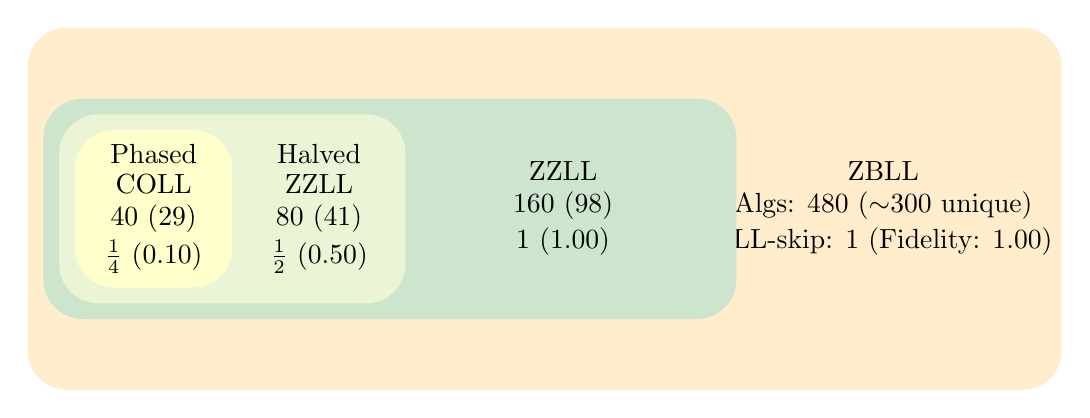
\begin{tikzpicture}
\node[very thin,draw=none,fill=Orange!20,align=center,anchor=west,minimum height=46mm,minimum width=\textwidth-1pt,rounded corners=5mm] at (-2mm,0) {\hspace{86mm}\shortstack[c]{ZBLL \\[1pt] Algs: 480 ($\sim$300 unique) \\ PLL-skip: $1$ (Fidelity: 1.00)}};
%
\node[very thin,draw=none,fill=Green!20,align=center,anchor=west,minimum height=28mm,minimum width=88mm,rounded corners=5mm] at (0,0) {\hspace{44mm}\shortstack[c]{ZZLL \\[1pt] 160 (98) \\ $1$ (1.00)}};
%
\node[very thin,draw=none,fill=YellowGreen!20,align=center,anchor=west,minimum height=24mm,minimum width=44mm,rounded corners=5mm] at (2mm,0) {\hspace{22mm}\shortstack[c]{Halved \\[1pt] ZZLL \\[1pt] 80 (41) \\ $\tfrac{1}{2}$ (0.50)}};
%
\node[very thin,draw=none,fill=Yellow!20,align=center,anchor=west,minimum size=20mm,rounded corners=5mm] at (4mm,0) {\shortstack[c]{Phased \\[1pt] COLL \\[1pt] 40 (29) \\ $\tfrac{1}{4}$ (0.10)}};
\end{tikzpicture}%
\\
\textit{Figure 1. Advanced Last Layer algorithmic sets compared}
\end{center}



\clearpage
\section*{Naming and recognition scheme of ZZLL algorithms}
\addcontentsline{toc}{section}{Recognition scheme}%

Let us look in detail at an exemplary entry from this reference and then remember the recognition of 7 non-trivial OLL classes, 40 COLL cases and 8 ZZLL layouts.
\vspace{16pt}%
\begin{center}%
% Args line: \coll{T.North}{\cU,\cF}{\cU,\cF}{\cL,\co,\cU}{\cR,\co,\cU}{
%    \draw[\cF] (TL) node[fill=\cF] {} -- (TR) node[fill=\cF] {};
%    \path (BL) node[fill=\cL] {} (BR) node[fill=\cR] {};
%}
\newlength{\osep}%
\setlength{\osep}{2mm}%
\readlist\lbu{\cU,\cF}%
\readlist\rbu{\cU,\cF}%
\readlist\flu{\cL,\co,\cU}%
\readlist\fru{\cR,\co,\cU}%
\hspace{-4mm}%
\begin{tikzpicture}[scale=\scl,baseline={([yshift=-2pt]CENTER)}]
    % --- --- --- Up yellow cross
    \fill[\cU] (1,3) -- ++({-(\asp-1)/2},3*\dep) -- ++(\asp,0) -- (2,3) -- cycle;
    \fill[\cU] (0,3) ++ ({-(\asp-1)/2},\dep) -- ++ ({-(\asp-1)/2},\dep) -- ++(2*\asp+1,0) -- ++({-(\asp-1)/2},-\dep) -- cycle;
    % --- --- --- LBU corner
    \fill[{\lbu[1]}] (0,2) ++({-(\asp-1)/2*3},3*\dep) -- ++(0,1) -- ++({+(\asp-1)/2},-\dep) -- ++(0,-1) -- cycle;
    \fill[{\lbu[2]}] (0,3) ++({-(\asp-1)/2*3},3*\dep) -- ++(\asp,0) -- ++({+(\asp-1)/6},-\dep) -- ++({-(2*\asp+1)/3},0) -- cycle;
    % --- --- --- RBU corner
    \fill[{\rbu[1]}] (3,2) ++({+(\asp-1)/2*3},3*\dep) -- ++(0,1) -- ++({-(\asp-1)/2},-\dep) -- ++(0,-1) -- cycle;
    \fill[{\rbu[2]}] (3,3) ++({+(\asp-1)/2*3},3*\dep) -- ++(-\asp,0) -- ++({-(\asp-1)/6},-\dep) -- ++({+(2*\asp+1)/3},0) -- cycle;
    % --- --- --- FLU corner
    \fill[{\flu[1]}] (0,2) rectangle (1,3);
    \fill[{\flu[2]}] (0,2) -- ++({-(\asp-1)/2},\dep) -- ++(0,1) -- ++({+(\asp-1)/2},-\dep) -- cycle;
    \fill[{\flu[3]}] (0,3) -- ++({-(\asp-1)/2},\dep) -- ++({(\asp+2)/3},0) -- ++({+(\asp-1)/6},-\dep) -- cycle;
    % --- --- --- FRU corner
    \fill[{\fru[1]}] (2,2) rectangle (3,3);
    \fill[{\fru[2]}] (3,2) -- ++({+(\asp-1)/2},\dep) -- ++(0,1) -- ++({-(\asp-1)/2},-\dep) -- cycle;
    \fill[{\fru[3]}] (3,3) -- ++({+(\asp-1)/2},\dep) -- ++({-(\asp+2)/3},0) -- ++({-(\asp-1)/6},-\dep) -- cycle;
    % --- --- --- LU edge
    \fill[\co] (0,2) ++({-(\asp-1)/2},\dep) -- ++({-(\asp-1)/2},\dep) -- ++(0,1) -- ++({+(\asp-1)/2},-\dep) -- cycle;
    % --- --- --- RU edge
    \fill[\co] (3,2) ++({+(\asp-1)/2},\dep) -- ++({+(\asp-1)/2},\dep) -- ++(0,1) -- ++({-(\asp-1)/2},-\dep) -- cycle;
    % --- --- --- FU edge
    \fill[\co] (1,2) rectangle (2,3);
    % === === === Front
    \tikzset{every path/.style={draw=White,thick}}
    \draw (0,2) rectangle (3,3);
    \draw (1,2) rectangle (2,3);
    % === === === Up
    \draw (0,3) -- ++({-(\asp-1)/2*3},3*\dep) -- ++(3*\asp,0) -- ++({-(\asp-1)/2*3},-3*\dep);
    \draw (0,3) ++ ({-(\asp-1)/2*1},1*\dep) -- ++(1*\asp+2,0);
    \draw (0,3) ++ ({-(\asp-1)/2*2},2*\dep) -- ++(2*\asp+1,0);
    \draw (1,3) -- ({1*\asp-(\asp-1)/2*3},3+3*\dep);
    \draw (2,3) -- ({2*\asp-(\asp-1)/2*3},3+3*\dep);
    % === === === Left
    \draw (0,2) -- ++({-(\asp-1)/2*3},3*\dep) -- ++(0,1);
    \draw (0,2) ++({-(\asp-1)/2*1},1*\dep) -- ++(0,1);
    \draw (0,2) ++({-(\asp-1)/2*2},2*\dep) -- ++(0,1);
    %~ \draw (0,1) -- ++({-(\asp-1)/2*3},3*\dep);
    \draw (0,2) -- ++({-(\asp-1)/2*3},3*\dep);
    % === === === Right
    \draw (3,2) -- ++({+(\asp-1)/2*3},3*\dep) -- ++(0,1);
    \draw (3,2) ++({+(\asp-1)/2*1},1*\dep) -- ++(0,1);
    \draw (3,2) ++({+(\asp-1)/2*2},2*\dep) -- ++(0,1);
    %~ \draw (3,1) -- ++({+(\asp-1)/2*3},3*\dep);
    \draw (3,2) -- ++({+(\asp-1)/2*3},3*\dep);
    %
    \coordinate (CENTER) at (3+1.5*\asp-1.5, 2.5+1.5*\dep);
    \useasboundingbox (current bounding box.north east) -- (current bounding box.north west) -- (current bounding box.south west) -- (current bounding box.south east) -- cycle;    % Freeze the bounding box
    \node[align=center,anchor=south,outer sep=0pt,draw=Black,thin,dashed,rounded corners=1mm] (TXT_COLL) at (1.5, 3+3*\dep+0.5715) {\bfseries T.North};
    %
    \draw[ultra thin,BBoxColor] (current bounding box.north east) -- (current bounding box.north west) -- (current bounding box.south west) -- (current bounding box.south east) -- cycle;
    %
    \draw[thin,Black] ([xshift=2pt]TXT_COLL.east) -- ++(1.1,0);
    \draw[Black,thin,dashed,rounded corners=1mm] ([shift={(+\osep,+\osep)}]current bounding box.north east) -- ([shift={(-\osep,+\osep)}]current bounding box.north west) -- ([shift={(-\osep,-\osep)}]current bounding box.south west) -- ([shift={(+\osep,-\osep)}]current bounding box.south east) -- cycle;
    \draw[thin,Black,-Stealth] ([yshift=-\osep-3pt]current bounding box.south) -- ++(0,-1) node[align=center,anchor=north] {COLL case};
\end{tikzpicture}%
\hspace{3.22mm}%
\begin{tikzpicture}[scale=\scl, baseline={([yshift=-2pt]CENTER)},%
                    every path/.style={line width=1.5mm,line cap=round},%
                    every node/.style={shape=rectangle,minimum size=5mm,rounded corners=1mm}]
    \coordinate (BL) at (-\sza,-\sza);
    \coordinate (BR) at (+\sza,-\sza);
    \coordinate (TL) at (-\sza,+\sza);
    \coordinate (TR) at (+\sza,+\sza);
    \draw[\cF] (TL) node[fill=\cF] {} -- (TR) node[fill=\cF] {};
    \path (BL) node[fill=\cL] (NBL) {} (BR) node[fill=\cR] {};
    %
    \coordinate (CENTER) at (0,0);
    \useasboundingbox (current bounding box.north east) -- (current bounding box.north west) -- (current bounding box.south west) -- (current bounding box.south east) -- cycle;    % Freeze the bounding box
    %
    \draw[ultra thin,BBoxColor] (current bounding box.north east) -- (current bounding box.north west) -- (current bounding box.south west) -- (current bounding box.south east) -- cycle;
    %
    \draw[Black,thin,dashed,rounded corners=1mm] ([shift={(+\osep,+\osep)}]current bounding box.north east) -- ([shift={(-\osep,+\osep)}]current bounding box.north west) -- ([shift={(-\osep,-\osep)}]current bounding box.south west) -- ([shift={(+\osep,-\osep)}]current bounding box.south east) -- cycle;
    \draw[thin,Black,-Stealth] ([shift={(-\osep,\osep)}]current bounding box.north west) -- ++(-0.5,0.8) -- ++(0.8,0) node[align=center,anchor=west] {COLL mnemonics};
    %
    \draw[very thin,Black,Stealth-,rounded corners=2mm] (BR) |- ([shift={(-5mm,-1cm)}]-\sza,-\sza) -- ++(-7mm,0) -| ++(-0.5-1.5*\asp+1.5,1) node[circle,fill=Black,scale=0.15] {};
    \draw[very thin,Black,Stealth-,rounded corners=2mm] (BL) |- ++(-12mm,+0.7cm) -| ++(-2.5-1.5*\asp+1.5,-0.7) node[circle,fill=Black,scale=0.15] {};
    \draw[very thin,Black,Stealth-,rounded corners=2mm] (TL) |- ++(-12mm,-0.7cm) -| ++({-5*(\asp-1)/4+5*\asp/12+1.0/12-3-1.5*\asp+1.5},+0.7-2*\sza+2.5*\dep+0.55) node[circle,fill=Black,scale=0.15] {};
    \draw[very thin,Black,Stealth-,rounded corners=2mm] (TR) |- ([shift={(-5mm,+0.9cm)}]-\sza,+\sza) -- ++(-7mm,0) -| ++({3+5*(\asp-1)/4-5*\asp/12-1.0/12-3-1.5*\asp+1.5},-0.9-2*\sza+2.5*\dep+0.55) node[circle,fill=Black,scale=0.15] {};
\end{tikzpicture}%
\hspace{6mm}%
% Args line: \zzll{\color{Grey} O/O}{\cU,\cF}{\cU,\cF}{\cL,\cB,\cU}{\cR,\cB,\cU}{\cF,\cB,\cR}{C/C}
\readlist\lbu{\cU,\cF}%
\readlist\rbu{\cU,\cF}%
\readlist\flu{\cL,\cB,\cU}%
\readlist\fru{\cR,\cB,\cU}%
\readlist\edg{\cF,\cB,\cR}%
\begin{tikzpicture}[scale=\scl,baseline={([yshift=-2pt]CENTER)}]
    %~ \useasboundingbox ({-(\asp-1)/2*3-0.7},2-0.2) rectangle ({3+(\asp-1)/2*3+0.7}, 3+3*\dep+0.2);
    % --- --- --- Up yellow cross
    \fill[\cU] (1,3) -- ++({-(\asp-1)/2},3*\dep) -- ++(\asp,0) -- (2,3) -- cycle;
    \fill[\cU] (0,3) ++ ({-(\asp-1)/2},\dep) -- ++ ({-(\asp-1)/2},\dep) -- ++(2*\asp+1,0) -- ++({-(\asp-1)/2},-\dep) -- cycle;
    % --- --- --- LBU corner
    \fill[{\lbu[1]}] (0,2) ++({-(\asp-1)/2*3},3*\dep) -- ++(0,1) -- ++({+(\asp-1)/2},-\dep) -- ++(0,-1) -- cycle;
    \fill[{\lbu[2]}] (0,3) ++({-(\asp-1)/2*3},3*\dep) -- ++(\asp,0) -- ++({+(\asp-1)/6},-\dep) -- ++({-(2*\asp+1)/3},0) -- cycle;
    % --- --- --- RBU corner
    \fill[{\rbu[1]}] (3,2) ++({+(\asp-1)/2*3},3*\dep) -- ++(0,1) -- ++({-(\asp-1)/2},-\dep) -- ++(0,-1) -- cycle;
    \fill[{\rbu[2]}] (3,3) ++({+(\asp-1)/2*3},3*\dep) -- ++(-\asp,0) -- ++({-(\asp-1)/6},-\dep) -- ++({+(2*\asp+1)/3},0) -- cycle;
    % --- --- --- FLU corner
    \fill[{\flu[1]}] (0,2) rectangle (1,3);
    \fill[{\flu[2]}] (0,2) -- ++({-(\asp-1)/2},\dep) -- ++(0,1) -- ++({+(\asp-1)/2},-\dep) -- cycle;
    \fill[{\flu[3]}] (0,3) -- ++({-(\asp-1)/2},\dep) -- ++({(\asp+2)/3},0) -- ++({+(\asp-1)/6},-\dep) -- cycle;
    % --- --- --- FRU corner
    \fill[{\fru[1]}] (2,2) rectangle (3,3);
    \fill[{\fru[2]}] (3,2) -- ++({+(\asp-1)/2},\dep) -- ++(0,1) -- ++({-(\asp-1)/2},-\dep) -- cycle;
    \fill[{\fru[3]}] (3,3) -- ++({+(\asp-1)/2},\dep) -- ++({-(\asp+2)/3},0) -- ++({-(\asp-1)/6},-\dep) -- cycle;
    % --- --- --- LU edge
    \fill[{\edg[1]}] (0,2) ++({-(\asp-1)/2},\dep) -- ++({-(\asp-1)/2},\dep) -- ++(0,1) -- ++({+(\asp-1)/2},-\dep) -- cycle;
    % --- --- --- RU edge
    \fill[{\edg[2]}] (3,2) ++({+(\asp-1)/2},\dep) -- ++({+(\asp-1)/2},\dep) -- ++(0,1) -- ++({-(\asp-1)/2},-\dep) -- cycle;
    % --- --- --- FU edge
    \fill[{\edg[3]}] (1,2) rectangle (2,3);
    % === === === Front
    \tikzset{every path/.style={draw=White,thick}}
    \draw (0,2) rectangle (3,3);
    \draw (1,2) rectangle (2,3);
    % === === === Up
    \draw (0,3) -- ++({-(\asp-1)/2*3},3*\dep) -- ++(3*\asp,0) -- ++({-(\asp-1)/2*3},-3*\dep);
    \draw (0,3) ++ ({-(\asp-1)/2*1},1*\dep) -- ++(1*\asp+2,0);
    \draw (0,3) ++ ({-(\asp-1)/2*2},2*\dep) -- ++(2*\asp+1,0);
    \draw (1,3) -- ({1*\asp-(\asp-1)/2*3},3+3*\dep);
    \draw (2,3) -- ({2*\asp-(\asp-1)/2*3},3+3*\dep);
    % === === === Left
    \draw (0,2) ++({-(\asp-1)/2*1},1*\dep) -- ++(0,1);
    \draw (0,2) ++({-(\asp-1)/2*2},2*\dep) -- ++(0,1);
    % === === === Right
    \draw (3,2) ++({+(\asp-1)/2*1},1*\dep) -- ++(0,1);
    \draw (3,2) ++({+(\asp-1)/2*2},2*\dep) -- ++(0,1);
    %
    \coordinate (CENTER) at (3+1.5*\asp-1.5+0.5, 2.5+1.5*\dep);
    \useasboundingbox ([xshift=9pt]current bounding box.north east) -- ([xshift=-9pt]current bounding box.north west) -- ([xshift=-9pt]current bounding box.south west) -- ([xshift=9pt]current bounding box.south east) -- cycle;    % Freeze the bounding box
    %
    \draw[ultra thin,BBoxColor] (current bounding box.north east) -- (current bounding box.north west) -- (current bounding box.south west) -- (current bounding box.south east) -- cycle;
    %
    \draw (0,2) -- ++({-(\asp-1)/2*3},3*\dep) node[pos=0.6,below,sloped,draw=Black,thin,dashed,rounded corners=1mm,inner sep=1pt,outer sep=1pt] (TXT_LEFT_MEMO) {\bfseries\color{Grey} O/O} -- ++(0,1);
    \draw (3,2) -- ++({+(\asp-1)/2*3},3*\dep) node[pos=0.6,below,sloped,draw=Black,thin,dashed,rounded corners=1mm,inner sep=1pt,outer sep=1pt] (TXT_RIGHT_MEMO) {\bfseries C/C} -- ++(0,1);
    \draw[thin,Black,-Stealth] (TXT_LEFT_MEMO.south) -- ++(-0.9,-0.6) -- ++(0,-1.25) node[align=center,anchor=north] {Left ZZLL mnemonic \\[-2pt] \scriptsize ({\color{Grey}\textbf{less convenient}})};
    \draw[thin,Black,-Stealth] (TXT_RIGHT_MEMO.south) -- ++(+0.9,-0.6) -- ++(0,-1.25) node[align=center,anchor=north] {Right ZZLL mnemonic \\[-2pt] \scriptsize (\textbf{preferred one})};
    %
    \draw[Black,thin,dashed,rounded corners=1mm] ([shift={(+\osep,+\osep)}]current bounding box.north east) -- ([shift={(-\osep,+\osep)}]current bounding box.north west) -- ([shift={(-\osep,-\osep)}]current bounding box.south west) -- ([shift={(+\osep,-\osep)}]current bounding box.south east) -- cycle;
    \draw[thin,Black,-Stealth] ([shift={(\osep,\osep)}]current bounding box.north east) -- ++(+0.5,0.8) -- ++(1,0) node[align=center,anchor=west] {ZZLL layout};
\end{tikzpicture}%
\hspace{5mm}%
\setlength{\alglen}{70mm}%
% Args line: \dual{U ~ (r'U'_2L') ~ D'_2 ~ (LU'_2L') ~ D'_2 ~ r^\mts_2}{U' ~ (lU^\mts_2R) ~ D^\mts_2 ~ (R'U^\mts_2R) ~ D^\mts_2 ~ l'_2}%
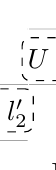
\begin{tikzpicture}[baseline={([yshift=-2pt]CENTER)}]
    \useasboundingbox (0,{-(1+3*\dep+0.4)/2*\scl}) rectangle (\alglen,{+(1+3*\dep+0.4)/2*\scl});    % Freeze the bounding box
    \coordinate (CENTER) at (0.5\alglen,0);
    %
    \draw[white] (0,0) coordinate (L) -- (\alglen,0) coordinate (R) coordinate[midway] (M);
    \node[anchor=south west,inner sep=0pt,outer sep=4pt,text depth=2pt,text height=9pt] (A) at ([xshift=-4pt]L) {$U ~ (r'U'_2L') ~ D'_2 ~ (LU'_2L') ~ D'_2 ~ r^\mts_2$};
    \node[anchor=north east,inner sep=0pt,outer sep=4pt,text depth=2pt,text height=9pt] (B) at ([xshift=+4pt]R) {$U' ~ (lU^\mts_2R) ~ D^\mts_2 ~ (R'U^\mts_2R) ~ D^\mts_2 ~ l'_2$};
    \draw[ultra thin,rounded corners=6pt] ([yshift=-0.5pt]current bounding box.north east) -| ([shift={(+4pt,-3pt)}]A.east) ++(0,6pt) |- ([xshift=-1pt]M) ++(2pt,0) -| ([shift={(-4pt,-3pt)}]B.west) ++(0,6pt) |- ([yshift=+0.5pt]current bounding box.south west);
    %
    \draw[ultra thin,BBoxColor] (current bounding box.north east) -- (current bounding box.north west) -- (current bounding box.south west) -- (current bounding box.south east) -- cycle;
    %
    \draw[Black,thin,dashed,rounded corners=1mm] ([shift={(-2pt,-2pt)}]A.north east) -- ([shift={(+2pt,-2pt)}]A.north west) -- ([shift={(+2pt,+1.5pt)}]A.south west) -- ([shift={(-2pt,+1.5pt)}]A.south east) -- cycle;
    \draw[Black,thin,dashed,rounded corners=1mm] ([shift={(-2pt,-1.5pt)}]B.north east) -- ([shift={(+2pt,-1.5pt)}]B.north west) -- ([shift={(+2pt,+2pt)}]B.south west) -- ([shift={(-2pt,+2pt)}]B.south east) -- cycle;
    \begin{scope}[scale=\scl]
        \draw[thin,Black,-Stealth] ([shift={(-4pt,-4pt)}]A.north east) -- ++(+0.7,+1.1) -- ++(1,0) node[align=center,anchor=west] {ZZLL Algorithm};
        \draw[thin,Black,-Stealth] ([shift={(+4pt,+4pt)}]B.south west) -- ++(-1.1,-1.1) -- ++(1,0) node[align=center,anchor=west] (TXT_MIRR) {Mirrored ZZLL algorithm \hspace{6mm} Mirrored ZZLL layout};
        \draw[thin,Black,decoration={brace,amplitude=11pt,mirror,raise=-2pt},decorate] (TXT_MIRR.south west) -- (TXT_MIRR.south east) node[midway,below,outer sep=8.7pt] {\scriptsize (for mirrorable algorithms/symmetric layouts only)};
    \end{scope}
\end{tikzpicture}%
\hspace{5mm}%
% Args line: \zzll{\color{Grey} C/C}{\cU,\cF}{\cU,\cF}{\cL,\cB,\cU}{\cR,\cB,\cU}{\cB,\cF,\cL}{O/O}%
\readlist\lbu{\cU,\cF}%
\readlist\rbu{\cU,\cF}%
\readlist\flu{\cL,\cB,\cU}%
\readlist\fru{\cR,\cB,\cU}%
\readlist\edg{\cB,\cF,\cL}%
\begin{tikzpicture}[scale=\scl,baseline={([yshift=-2pt]CENTER)}]
    %~ \useasboundingbox ({-(\asp-1)/2*3-0.7},2-0.2) rectangle ({3+(\asp-1)/2*3+0.7}, 3+3*\dep+0.2);
    % --- --- --- Up yellow cross
    \fill[\cU] (1,3) -- ++({-(\asp-1)/2},3*\dep) -- ++(\asp,0) -- (2,3) -- cycle;
    \fill[\cU] (0,3) ++ ({-(\asp-1)/2},\dep) -- ++ ({-(\asp-1)/2},\dep) -- ++(2*\asp+1,0) -- ++({-(\asp-1)/2},-\dep) -- cycle;
    % --- --- --- LBU corner
    \fill[{\lbu[1]}] (0,2) ++({-(\asp-1)/2*3},3*\dep) -- ++(0,1) -- ++({+(\asp-1)/2},-\dep) -- ++(0,-1) -- cycle;
    \fill[{\lbu[2]}] (0,3) ++({-(\asp-1)/2*3},3*\dep) -- ++(\asp,0) -- ++({+(\asp-1)/6},-\dep) -- ++({-(2*\asp+1)/3},0) -- cycle;
    % --- --- --- RBU corner
    \fill[{\rbu[1]}] (3,2) ++({+(\asp-1)/2*3},3*\dep) -- ++(0,1) -- ++({-(\asp-1)/2},-\dep) -- ++(0,-1) -- cycle;
    \fill[{\rbu[2]}] (3,3) ++({+(\asp-1)/2*3},3*\dep) -- ++(-\asp,0) -- ++({-(\asp-1)/6},-\dep) -- ++({+(2*\asp+1)/3},0) -- cycle;
    % --- --- --- FLU corner
    \fill[{\flu[1]}] (0,2) rectangle (1,3);
    \fill[{\flu[2]}] (0,2) -- ++({-(\asp-1)/2},\dep) -- ++(0,1) -- ++({+(\asp-1)/2},-\dep) -- cycle;
    \fill[{\flu[3]}] (0,3) -- ++({-(\asp-1)/2},\dep) -- ++({(\asp+2)/3},0) -- ++({+(\asp-1)/6},-\dep) -- cycle;
    % --- --- --- FRU corner
    \fill[{\fru[1]}] (2,2) rectangle (3,3);
    \fill[{\fru[2]}] (3,2) -- ++({+(\asp-1)/2},\dep) -- ++(0,1) -- ++({-(\asp-1)/2},-\dep) -- cycle;
    \fill[{\fru[3]}] (3,3) -- ++({+(\asp-1)/2},\dep) -- ++({-(\asp+2)/3},0) -- ++({-(\asp-1)/6},-\dep) -- cycle;
    % --- --- --- LU edge
    \fill[{\edg[1]}] (0,2) ++({-(\asp-1)/2},\dep) -- ++({-(\asp-1)/2},\dep) -- ++(0,1) -- ++({+(\asp-1)/2},-\dep) -- cycle;
    % --- --- --- RU edge
    \fill[{\edg[2]}] (3,2) ++({+(\asp-1)/2},\dep) -- ++({+(\asp-1)/2},\dep) -- ++(0,1) -- ++({-(\asp-1)/2},-\dep) -- cycle;
    % --- --- --- FU edge
    \fill[{\edg[3]}] (1,2) rectangle (2,3);
    % === === === Front
    \tikzset{every path/.style={draw=White,thick}}
    \draw (0,2) rectangle (3,3);
    \draw (1,2) rectangle (2,3);
    % === === === Up
    \draw (0,3) -- ++({-(\asp-1)/2*3},3*\dep) -- ++(3*\asp,0) -- ++({-(\asp-1)/2*3},-3*\dep);
    \draw (0,3) ++ ({-(\asp-1)/2*1},1*\dep) -- ++(1*\asp+2,0);
    \draw (0,3) ++ ({-(\asp-1)/2*2},2*\dep) -- ++(2*\asp+1,0);
    \draw (1,3) -- ({1*\asp-(\asp-1)/2*3},3+3*\dep);
    \draw (2,3) -- ({2*\asp-(\asp-1)/2*3},3+3*\dep);
    % === === === Left
    \draw (0,2) ++({-(\asp-1)/2*1},1*\dep) -- ++(0,1);
    \draw (0,2) ++({-(\asp-1)/2*2},2*\dep) -- ++(0,1);
    % === === === Right
    \draw (3,2) ++({+(\asp-1)/2*1},1*\dep) -- ++(0,1);
    \draw (3,2) ++({+(\asp-1)/2*2},2*\dep) -- ++(0,1);
    %
    \coordinate (CENTER) at (3+1.5*\asp-1.5+0.5, 2.5+1.5*\dep);
    \useasboundingbox ([xshift=9pt]current bounding box.north east) -- ([xshift=-9pt]current bounding box.north west) -- ([xshift=-9pt]current bounding box.south west) -- ([xshift=9pt]current bounding box.south east) -- cycle;    % Freeze the bounding box
    %
    \draw[ultra thin,BBoxColor] (current bounding box.north east) -- (current bounding box.north west) -- (current bounding box.south west) -- (current bounding box.south east) -- cycle;
    %
    \draw (0,2) -- ++({-(\asp-1)/2*3},3*\dep) node[pos=0.6,below,sloped] (TXT_LEFT_MEMO) {\bfseries\color{Grey} C/C} -- ++(0,1);
    \draw (3,2) -- ++({+(\asp-1)/2*3},3*\dep) node[pos=0.6,below,sloped] (TXT_RIGHT_MEMO) {\bfseries O/O} -- ++(0,1);
    %
    \draw[Black,thin,dashed,rounded corners=1mm] ([shift={(+\osep,+\osep)}]current bounding box.north east) -- ([shift={(-\osep,+\osep)}]current bounding box.north west) -- ([shift={(-\osep,-\osep)}]current bounding box.south west) -- ([shift={(+\osep,-\osep)}]current bounding box.south east) -- cycle;
    \draw[thin,Black,-Stealth] ([shift={(-\osep,-\osep)}]current bounding box.south west) -- ++(-1.0,-0.8) -- ++(0.7,0);
\end{tikzpicture}%
\\[44pt]%
\textit{Figure 2. Reference entry explained}%
\end{center}%
The complete naming of entry on figure 2 reads \textbf{T.North.C/C} (for the first algorithm) and \textbf{T.North.O/O} (mirrored one). Such naming scheme closely follows the recognition order \textbf{OLL.COLL.ZZLL}. In the family of ZZ speedsolving methods only the following 7 non-trivial OLL classes appear (the edges have been oriented during the EOLine stage of any ZZ solve).
\begin{center}
\textbf{T} \hspace{\widthof{\bfseries Pi}-\widthof{\bfseries T}}%
\oll{\cU,\cs}{\cU,\cs}{\cs,\co,\cU}{\cs,\co,\cU}{ \path (UBL) node {1} (FLU) node {2} (UBR) node {3} (FRU) node {4}; }\hfill%
\textbf{U} %
\oll{\co,\cs}{\co,\cs}{\cs,\co,\cU}{\cs,\co,\cU}{ \path (UBL) node {1} (FLU) node {2} (UBR) node {3} (FRU) node {4}; }\hfill%
\textbf{L} %
\oll{\co,\cU}{\co,\cs}{\cs,\cU,\cs}{\cs,\co,\cU}{ \path (UFL) node {1} (FLU) node {2} (UBR) node {3} (FRU) node {4}; }\hfill%
\textbf{H} %
\oll{\co,\cs}{\co,\cs}{\cU,\co,\cs}{\cU,\co,\cs}{ \path (UBL) node {1} (UFL) node {2} (UBR) node {3} (UFR) node {4}; }%
\\[4pt]%
\textbf{Pi} %
\oll{\cU,\cs}{\co,\cs}{\co,\cU,\cs}{\cU,\co,\cs}{ \path (UBL) node {1} (UFL) node {2} (UBR) node {3} (UFR) node {4}; }\hfill%
\textbf{S} (Sune) %
\oll{\co,\cU}{\cU,\cs}{\cs,\cU,\cs}{\cU,\co,\cs}{ \path (UFL) node {1} (FLU) node {2} (UBR) node {3} (UFR) node {4}; }\hfill%
\textbf{As} (Anti-sune) %
\oll{\cU,\cs}{\co,\cU}{\cU,\co,\cs}{\cs,\cU,\cs}{ \path (UBL) node {1} (UFL) node {2} (UFR) node {3} (FRU) node {4}; }%
\\[5pt]%
\textit{Figure 3. Recognition of OLL class and columnwise mapping of corner stickers to COLL patterns}
\end{center}
After OLL class is detected one distinguishes COLL case by comparing dark-gray highlighted stickers (on figure 3) to those of COLL mnemonic pattern. As shown here, exact mapping of COLL-determining stickers depends on the OLL class. Actual patterns may vary in colors, only the \emph{relative} color of any two stickers matters (are they same, opposite or adjacent).
\begin{center}
\setlength{\tabcolsep}{9pt}%
\begin{tabular}{crrrrrr}
\toprule\addlinespace[1pt]
\addlinespace[1pt]
OLL Class & \multicolumn{6}{c}{COLL Cases} \\
\midrule
\textbf{T} &
\textbf{Rows} \collmnemo{
    \draw[\cF] (BL) node[fill=\cF] {} -- (BR) node[fill=\cF] {};
    \draw[\cB] (TL) node[fill=\cB] {} -- (TR) node[fill=\cB] {};
} &
\textbf{Cols} \collmnemo{
    \draw[\cF] (BL) node[fill=\cF] {} -- (TL) node[fill=\cF] {};
    \draw[\cB] (BR) node[fill=\cB] {} -- (TR) node[fill=\cB] {};
} &
\textbf{North} \collmnemo{
    \draw[\cF] (TL) node[fill=\cF] {} -- (TR) node[fill=\cF] {};
    \path      (BL) node[fill=\cL] {}    (BR) node[fill=\cR] {};
} &
\textbf{South} \collmnemo{
    \draw[\cF] (BL) node[fill=\cF] {} -- (BR) node[fill=\cF] {};
    \path      (TL) node[fill=\cR] {}    (TR) node[fill=\cL] {};
} &
\textbf{West} \collmnemo{
    \draw[\cF] (BL) node[fill=\cF] {} -- (TL) node[fill=\cF] {};
    \path      (BR) node[fill=\cR] {}    (TR) node[fill=\cL] {};
} &
\textbf{East} \collmnemo{
    \draw[\cF] (BR) node[fill=\cF] {} -- (TR) node[fill=\cF] {};
    \path      (BL) node[fill=\cL] {} -- (TL) node[fill=\cR] {};
} \\
\midrule
\textbf{U} &
\textbf{Rows} \collmnemo{
    \draw[\cF] (BL) node[fill=\cF] {} -- (BR) node[fill=\cF] {};
    \draw[\cB] (TL) node[fill=\cB] {} -- (TR) node[fill=\cB] {};
} &
\textbf{Cross} \collmnemo{
    \draw[\cB] (BL) node[fill=\cB] {} -- (TR) node[fill=\cB] {};
    \draw[\cF] (BR) node[fill=\cF] {} -- (TL) node[fill=\cF] {};
} &
\textbf{North} \collmnemo{
    \draw[\cF] (TL) node[fill=\cF] {} -- (TR) node[fill=\cF] {};
    \path      (BL) node[fill=\cL] {}    (BR) node[fill=\cR] {};
} &
\textbf{South} \collmnemo{
    \draw[\cF] (BL) node[fill=\cF] {} -- (BR) node[fill=\cF] {};
    \path      (TL) node[fill=\cL] {}    (TR) node[fill=\cR] {};
} &
\textbf{Slash} \collmnemo{
    \draw[\cF] (BL) node[fill=\cF] {} -- (TR) node[fill=\cF] {};
    \path      (BR) node[fill=\cR] {}    (TL) node[fill=\cL] {};
} &
\makecell[c]{\textbf{Back} \\ \textbf{slash}} \collmnemo{
    \draw[\cF] (BR) node[fill=\cF] {} -- (TL) node[fill=\cF] {};
    \path      (BL) node[fill=\cL] {}    (TR) node[fill=\cR] {};
} \\
\midrule
\textbf{L} &
\makecell[c]{\textbf{North} \\ \textbf{Opp.}} \collmnemo{
    \draw[\cF] (TL) node[fill=\cF] {} -- (TR) node[fill=\cF] {};
    \path      (BL) node[fill=\cL] {}    (BR) node[fill=\cR] {};
} &
\makecell[c]{\textbf{North} \\ \textbf{Adj.}} \collmnemo{
    \draw[\cF] (TL) node[fill=\cF] {} -- (TR) node[fill=\cF] {};
    \path      (BL) node[fill=\cL] {}    (BR) node[fill=\cB] {};
} &
\makecell[c]{\textbf{Opp.} \\ \textbf{Cross}} \collmnemo{
    \path      (BR) node[fill=\cF] {}    (BL) node[fill=\cR] {};
    \path      (TR) node[fill=\cL] {}    (TL) node[fill=\cB] {};
} &
\makecell[c]{\textbf{Opp.} \\ \textbf{Rows}} \collmnemo{
    \path      (BR) node[fill=\cF] {}    (BL) node[fill=\cB] {};
    \path      (TR) node[fill=\cR] {}    (TL) node[fill=\cL] {};
} &
\makecell[c]{\textbf{Slice} \\ \textbf{Adj.}} \collmnemo{
    \draw[\cF] (BR) node[fill=\cF] {} -- (TL) node[fill=\cF] {};
    \path      (BL) node[fill=\cL] {}    (TR) node[fill=\cB] {};
} &
\makecell[c]{\textbf{Slice} \\ \textbf{Opp.}} \collmnemo{
    \draw[\cF] (BR) node[fill=\cF] {} -- (TL) node[fill=\cF] {};
    \path      (BL) node[fill=\cL] {}    (TR) node[fill=\cR] {};
} \\
\midrule
\textbf{H} &
\textbf{Rows} \collmnemo{
    \draw[\cF] (BL) node[fill=\cF] {} -- (BR) node[fill=\cF] {};
    \draw[\cB] (TL) node[fill=\cB] {} -- (TR) node[fill=\cB] {};
} &
\textbf{Cols} \collmnemo{
    \draw[\cF] (BL) node[fill=\cF] {} -- (TL) node[fill=\cF] {};
    \draw[\cB] (BR) node[fill=\cB] {} -- (TR) node[fill=\cB] {};
} &
\textbf{South} \collmnemo{
    \draw[\cF] (BL) node[fill=\cF] {} -- (BR) node[fill=\cF] {};
    \path      (TL) node[fill=\cL] {}    (TR) node[fill=\cR] {};
} &
\textbf{West} \collmnemo{
    \draw[\cF] (BL) node[fill=\cF] {} -- (TL) node[fill=\cF] {};
    \path      (BR) node[fill=\cL] {} -- (TR) node[fill=\cR] {};
} & & \\
\midrule
\textbf{Pi} &
\textbf{Cols} \collmnemo{
    \draw[\cF] (BL) node[fill=\cF] {} -- (TL) node[fill=\cF] {};
    \draw[\cB] (BR) node[fill=\cB] {} -- (TR) node[fill=\cB] {};
} &
\textbf{Cross} \collmnemo{
    \draw[\cB] (BL) node[fill=\cB] {} -- (TR) node[fill=\cB] {};
    \draw[\cF] (BR) node[fill=\cF] {} -- (TL) node[fill=\cF] {};
} &
\textbf{West} \collmnemo{
    \draw[\cF] (BL) node[fill=\cF] {} -- (TL) node[fill=\cF] {};
    \path      (BR) node[fill=\cL] {}    (TR) node[fill=\cR] {};
} &
\textbf{East} \collmnemo{
    \draw[\cF] (BR) node[fill=\cF] {} -- (TR) node[fill=\cF] {};
    \path      (BL) node[fill=\cL] {} -- (TL) node[fill=\cR] {};
} &
\textbf{Slash} \collmnemo{
    \draw[\cF] (BL) node[fill=\cF] {} -- (TR) node[fill=\cF] {};
    \path      (BR) node[fill=\cL] {}    (TL) node[fill=\cR] {};
} &
\makecell[c]{\textbf{Back} \\ \textbf{slash}} \collmnemo{
    \draw[\cF] (BR) node[fill=\cF] {} -- (TL) node[fill=\cF] {};
    \path      (BL) node[fill=\cL] {}    (TR) node[fill=\cR] {};
} \\
\midrule
\textbf{S} and \textbf{As} &
\makecell[c]{\textbf{South} \\ \textbf{Opp.}} \collmnemo{
    \draw[\cF] (BL) node[fill=\cF] {} -- (BR) node[fill=\cF] {};
    \path      (TL) node[fill=\cR] {}    (TR) node[fill=\cL] {};
} &
\makecell[c]{\textbf{South} \\ \textbf{Adj.}} \collmnemo{
    \draw[\cF] (BL) node[fill=\cF] {} -- (BR) node[fill=\cF] {};
    \path      (TL) node[fill=\cR] {}    (TR) node[fill=\cB] {};
} &
\makecell[c]{\textbf{Opp.} \\ \textbf{Cross}} \collmnemo{
    \path      (BL) node[fill=\cB] {}    (BR) node[fill=\cR] {};
    \path      (TL) node[fill=\cL] {}    (TR) node[fill=\cF] {};
} &
\makecell[c]{\textbf{Opp.} \\ \textbf{Rows}} \collmnemo{
    \path      (BL) node[fill=\cB] {}    (BR) node[fill=\cF] {};
    \path      (TL) node[fill=\cL] {}    (TR) node[fill=\cR] {};
} &
\makecell[c]{\textbf{Slice} \\ \textbf{Adj.}} \collmnemo{
    \draw[\cF] (BL) node[fill=\cF] {} -- (TR) node[fill=\cF] {};
    \path      (TL) node[fill=\cR] {}    (BR) node[fill=\cB] {};
} &
\makecell[c]{\textbf{Slice} \\ \textbf{Opp.}} \collmnemo{
    \draw[\cF] (BL) node[fill=\cF] {} -- (TR) node[fill=\cF] {};
    \path      (TL) node[fill=\cR] {}    (BR) node[fill=\cL] {};
} \\
\bottomrule
\end{tabular}
\end{center}
Finally, one classifies ZZLL layout of the COLL case met. Each of 40 COLL cases comprises 4 ZZLL layouts. However, there are 8 kinds of ZZLL layouts (not mentioning 3 possible corner rotations) since COLL cases may have either even or odd combination of their edge and corner parities. The next table shows principal ZZLL layouts and their mnemonics.
\begin{center}
\setlength{\tabcolsep}{8pt}%
\begin{tabular}{r!{\hspace{8pt}}rr!{\hspace{24pt}}rr}
\toprule\addlinespace[1pt]
\addlinespace[1pt]
& \multicolumn{2}{c}{ZZLL layouts type \textbf{a/b}} & \multicolumn{2}{c}{ZZLL layouts type \textbf{a$\bm\times$b}} \\
\midrule
Even: &
\zzllmnemo{\bfseries C/C}{\cF,\cU,\cR}{\cF,\cR}{ \path (EL) node {a} (CL) node {a} (CR) node {b} (ER) node {b}; } &
\zzllmnemo{\bfseries O/O}{\cF,\cU,\cR}{\cB,\cL}{ \path (EL) node {a} (CL) node {a} (CR) node {b} (ER) node {b}; } &
\zzllmnemo{\bfseries C\x C}{\cF,\cU,\cR}{\cR,\cF}{ \path (EL) node {a} (CL) node {b} (CR) node {a} (ER) node {b}; } &
\zzllmnemo{\bfseries O\x O}{\cF,\cU,\cR}{\cL,\cB}{ \path (EL) node {a} (CL) node {b} (CR) node {a} (ER) node {b}; } \\
\addlinespace[2pt]
Odd: &
\zzllmnemo{\bfseries C/O}{\cF,\cU,\cR}{\cF,\cL}{ \path (EL) node {a} (CL) node {a} (CR) node {b} (ER) node {b}; } &
\zzllmnemo{\bfseries O/C}{\cF,\cU,\cR}{\cB,\cR}{ \path (EL) node {a} (CL) node {a} (CR) node {b} (ER) node {b}; } &
\zzllmnemo{\bfseries C\x O}{\cF,\cU,\cR}{\cR,\cB}{ \path (EL) node {a} (CL) node {b} (CR) node {a} (ER) node {b}; } &
\zzllmnemo{\bfseries O\x C}{\cF,\cU,\cR}{\cL,\cF}{ \path (EL) node {a} (CL) node {b} (CR) node {a} (ER) node {b}; } \\
\midrule
\makecell[r]{Rotated corner: \\ \scriptsize (even/odd as well)} &
\zzllmnemo{\bfseries a/b}{\cU,\cs,\cs}{\cs,\cs}{ \path (EL) node {a} (CT) node {a} (CR) node {b} (ER) node {b}; } &
\zzllmnemo{\bfseries a/b}{\cs,\cs,\cU}{\cs,\cs}{ \path (EL) node {a} (CL) node {a} (CT) node {b} (ER) node {b}; } &
\zzllmnemo{\bfseries a$\bm\times$b}{\cU,\cs,\cs}{\cs,\cs}{ \path (EL) node {a} (CT) node {b} (CR) node {a} (ER) node {b}; } &
\zzllmnemo{\bfseries a$\bm\times$b}{\cs,\cs,\cU}{\cs,\cs}{ \path (EL) node {a} (CL) node {b} (CT) node {a} (ER) node {b}; } \\
\bottomrule
\end{tabular}
\end{center}
Again, only the relations between colors matter: \textbf{C} = same/`correct', \textbf{O} = opposite. This reference provides two mnemonics for each ZZLL layout: left FL and right FR (see figure 2). It is a matter of habit to recognize particular ZZLL layout by its FL or FR mnemonic. Author's favourite mnemonics are typeset \textbf{in bold} whereas less convenient ones are {\color{Grey}\textbf{paled}}.

\section*{Internal ZZLL structure}
\addcontentsline{toc}{section}{ZZLL structure}%

As already mentioned, ZZLL algorithmic set can be factored as 40 COLL cases expanded into 4 ZZLL layouts each. Fortunately, there are only 36 self-mirroring algorithms, i.e.\,$160 = 36 + 2\cdot 62$ and one has to learn $36+62$ unique algs. Furthemore, just 32 algorithms are self-inverting, whereas the rest $160 - 32 = 2\cdot 64$ algs split into 64 `forward/inverse' pairs. Such internal relationships between 160 ZZLL algorithms are illustrated on figure 4 as follows: mutually mirroring algs' mnemonics are connected with solid lines, mutually inverting ones --- with dashed lines. Self-mirroring/self-inverting algs miss their solid/dashed lines respectively. The 20 disconnected algorithms are self-inverting and self-mirroring at the same time and cannot be learned in pairs. In contrast, $64 = 4\cdot 16$ algs can be practiced not only in pairs, but already in quartets.
\begin{center}
\vfill%
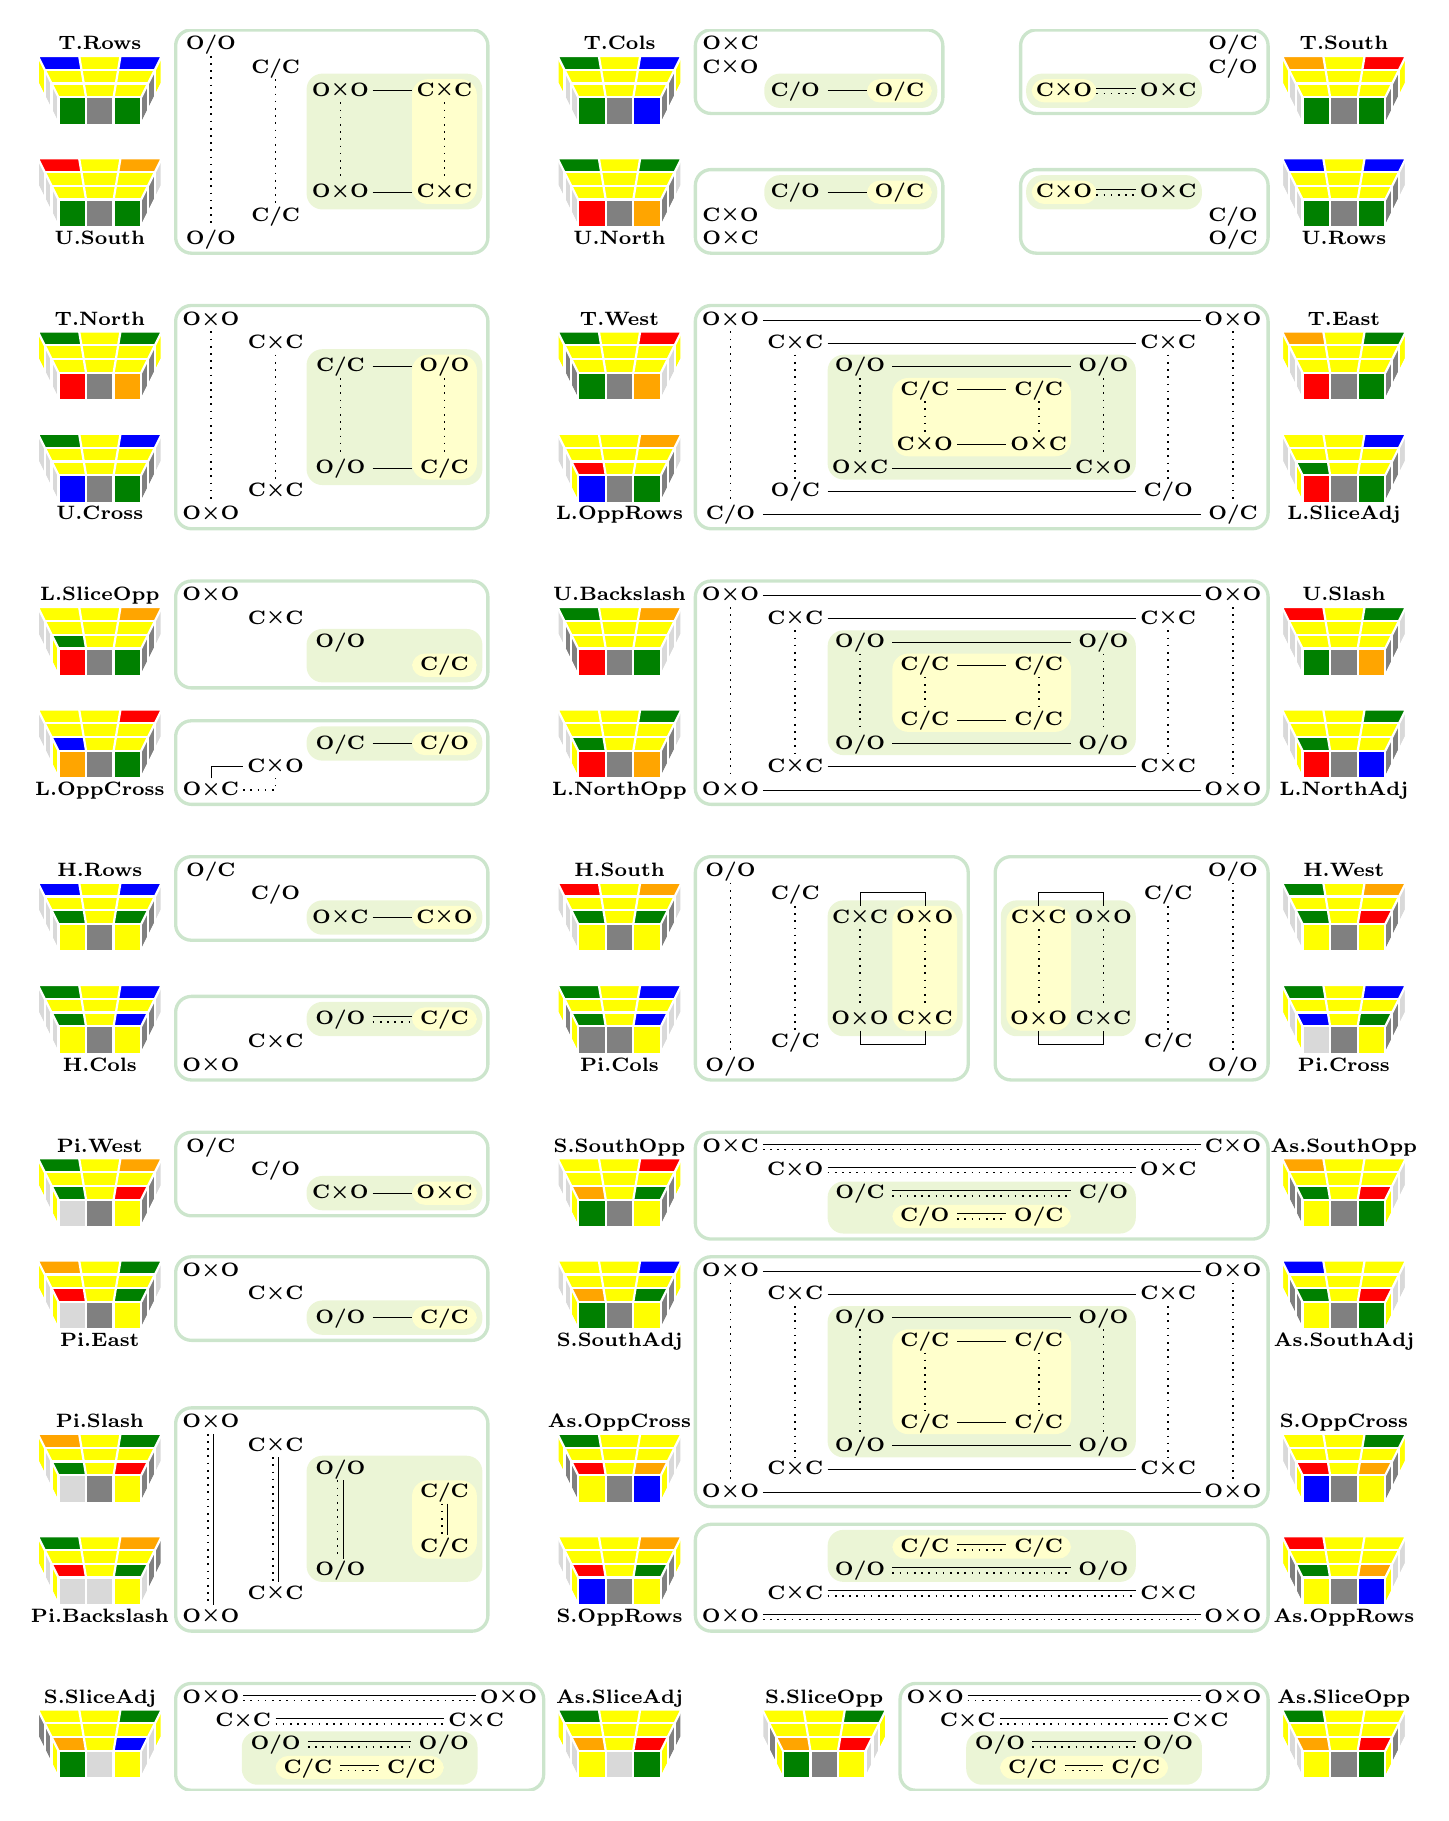
\begin{tikzpicture}[every node/.style={text depth=1pt,text height=5pt,inner sep=1pt,minimum width=2.3em,align=center,font=\scriptsize}]
\newcommand{\colone}{-6.8}
\newcommand{\coltwo}{-0.2}
\newcommand{\colthree}{9}
\newcommand{\pairoffset}{-3.5}
\newcommand{\singleoffset}{-1.3}
\newlength{\plainshift}\setlength{\plainshift}{5mm}
\newlength{\layoutsshift}\setlength{\layoutsshift}{6pt}
% === === === Single T.Cols
\pic[local bounding box=T_COLS] at (\coltwo,0) {collmini={\cU,\cF}{\cU,\cB}{\cF,\co,\cU}{\cB,\cs,\cU}{\co,\cs,\cs}};
\node[above] (T_COLS_NAME) at (T_COLS.north) {\bfseries T.Cols};
\node[above right] (T_COLS_OxC) at ([xshift=\layoutsshift]T_COLS.north east) {\bfseries O\x C};
\node[below] (T_COLS_CxO) at (T_COLS_OxC.south) {\bfseries C\x O};
\node[below right] (T_COLS_C/O) at (T_COLS_CxO.south east) {\bfseries C/O};
\node[right,xshift=\plainshift] (T_COLS_O/C) at (T_COLS_C/O.east) {\bfseries O/C};
%
\draw[very thin,Black] (T_COLS_C/O) -- (T_COLS_O/C);
%
\begin{scope}[on background layer]
\draw[very thick,Green!20,rounded corners=2mm] ([shift={(-1pt,+1pt)}]T_COLS_OxC.north west) rectangle ([shift={(+4pt,-4pt)}]T_COLS_O/C.south east);
\fill[YellowGreen!20,rounded corners=2mm] ([shift={(+0.5pt,+2pt)}]T_COLS_C/O.north west) rectangle ([shift={(+2pt,-2pt)}]T_COLS_O/C.south east);
\fill[Yellow!20,rounded corners=1.6mm] (T_COLS_O/C.north west) rectangle (T_COLS_O/C.south east);
\end{scope}
% === === === Single T.South
\pic[local bounding box=T_SOUTH] at (\colthree,0) {collmini={\cU,\cR}{\cU,\cL}{\cF,\co,\cU}{\cF,\cs,\cU}{\co,\cs,\cs}};
\node[above] (T_SOUTH_NAME) at (T_SOUTH.north) {\bfseries T.South};
\node[above left] (T_SOUTH_O/C) at ([xshift=-\layoutsshift]T_SOUTH.north west) {\bfseries O/C};
\node[below] (T_SOUTH_C/O) at (T_SOUTH_O/C.south) {\bfseries C/O};
\node[below left] (T_SOUTH_OxC) at (T_SOUTH_C/O.south west) {\bfseries O\x C};
\node[left,xshift=-\plainshift] (T_SOUTH_CxO) at (T_SOUTH_OxC.west) {\bfseries C\x O};
%
\draw[very thin,Black] ([yshift=1pt]T_SOUTH_CxO.east) -- ([yshift=1pt]T_SOUTH_OxC.west);
\draw[line width=0.6pt,dotted,Black] ([yshift=-1pt]T_SOUTH_CxO.east) -- ([yshift=-1pt]T_SOUTH_OxC.west);
%
\begin{scope}[on background layer]
\draw[very thick,Green!20,rounded corners=2mm] ([shift={(+1pt,+1pt)}]T_SOUTH_O/C.north east) rectangle ([shift={(-4pt,-4pt)}]T_SOUTH_CxO.south west);
\fill[YellowGreen!20,rounded corners=2mm] ([shift={(+0.5pt,+2pt)}]T_SOUTH_OxC.north east) rectangle ([shift={(-2pt,-2pt)}]T_SOUTH_CxO.south west);
\fill[Yellow!20,rounded corners=1.6mm] (T_SOUTH_CxO.north east) rectangle (T_SOUTH_CxO.south west);
\end{scope}
% === === === Single U.North
\pic[local bounding box=U_NORTH] at (\coltwo,\singleoffset) {collmini={\co,\cF}{\co,\cF}{\cL,\co,\cU}{\cR,\cs,\cU}{\co,\cs,\cs}};
\node[below] (U_NORTH_NAME) at (U_NORTH.south) {\bfseries U.North};
\node[below right] (U_NORTH_OxC) at ([xshift=\layoutsshift]U_NORTH.south east) {\bfseries O\x C};
\node[above] (U_NORTH_CxO) at (U_NORTH_OxC.north) {\bfseries C\x O};
\node[above right] (U_NORTH_C/O) at (U_NORTH_CxO.north east) {\bfseries C/O};
\node[right,xshift=\plainshift] (U_NORTH_O/C) at (U_NORTH_C/O.east) {\bfseries O/C};
%
\draw[very thin,Black] (U_NORTH_C/O) -- (U_NORTH_O/C);
%
\begin{scope}[on background layer]
\draw[very thick,Green!20,rounded corners=2mm] ([shift={(-1pt,-1pt)}]U_NORTH_OxC.south west) rectangle ([shift={(+4pt,+4pt)}]U_NORTH_O/C.north east);
\fill[YellowGreen!20,rounded corners=2mm] ([shift={(+0.5pt,+2pt)}]U_NORTH_C/O.north west) rectangle ([shift={(+2pt,-2pt)}]U_NORTH_O/C.south east);
\fill[Yellow!20,rounded corners=1.6mm] (U_NORTH_O/C.north west) rectangle (U_NORTH_O/C.south east);
\end{scope}
% === === === Single U.Rows
\pic[local bounding box=U_ROWS] at (\colthree,\singleoffset) {collmini={\co,\cB}{\co,\cB}{\cF,\co,\cU}{\cF,\cs,\cU}{\co,\cs,\cs}};
\node[below] (U_ROWS_NAME) at (U_ROWS.south) {\bfseries U.Rows};
\node[below left] (U_ROWS_O/C) at ([xshift=-\layoutsshift]U_ROWS.south west) {\bfseries O/C};
\node[above] (U_ROWS_C/O) at (U_ROWS_O/C.north) {\bfseries C/O};
\node[above left] (U_ROWS_OxC) at (U_ROWS_C/O.north west) {\bfseries O\x C};
\node[left,xshift=-\plainshift] (U_ROWS_CxO) at (U_ROWS_OxC.west) {\bfseries C\x O};
%
\draw[very thin,Black] ([yshift=1pt]U_ROWS_CxO.east) -- ([yshift=1pt]U_ROWS_OxC.west);
\draw[line width=0.6pt,dotted,Black] ([yshift=-1pt]U_ROWS_CxO.east) -- ([yshift=-1pt]U_ROWS_OxC.west);
%
\begin{scope}[on background layer]
\draw[very thick,Green!20,rounded corners=2mm] ([shift={(+1pt,-1pt)}]U_ROWS_O/C.south east) rectangle ([shift={(-4pt,+4pt)}]U_ROWS_CxO.north west);
\fill[YellowGreen!20,rounded corners=2mm] ([shift={(+0.5pt,-2pt)}]U_ROWS_OxC.south east) rectangle ([shift={(-2pt,+2pt)}]U_ROWS_CxO.north west);
\fill[Yellow!20,rounded corners=1.6mm] (U_ROWS_CxO.north east) rectangle (U_ROWS_CxO.south west);
\end{scope}
% === === === Pair T.Rows over U.South
\pic[local bounding box=T_ROWS] at (\colone,0) {collmini={\cU,\cB}{\cU,\cB}{\cF,\co,\cU}{\cF,\cs,\cU}{\co,\cs,\cs}};
\node[above] (T_ROWS_NAME) at (T_ROWS.north) {\bfseries T.Rows};
\node[above right] (T_ROWS_O/O) at ([xshift=\layoutsshift]T_ROWS.north east) {\bfseries O/O};
\node[below right] (T_ROWS_C/C) at (T_ROWS_O/O.south east) {\bfseries C/C};
\node[below right] (T_ROWS_OxO) at (T_ROWS_C/C.south east) {\bfseries O\x O};
\node[right,xshift=\plainshift] (T_ROWS_CxC) at (T_ROWS_OxO.east) {\bfseries C\x C};
%
\pic[local bounding box=U_SOUTH] at (\colone,\singleoffset) {collmini={\co,\cL}{\co,\cR}{\cF,\co,\cU}{\cF,\cs,\cU}{\co,\cs,\cs}};
\node[below] (U_SOUTH_NAME) at (U_SOUTH.south) {\bfseries U.South};
\node[below right] (U_SOUTH_O/O) at ([xshift=\layoutsshift]U_SOUTH.south east) {\bfseries O/O};
\node[above right] (U_SOUTH_C/C) at (U_SOUTH_O/O.north east) {\bfseries C/C};
\node[above right] (U_SOUTH_OxO) at (U_SOUTH_C/C.north east) {\bfseries O\x O};
\node[right,xshift=\plainshift] (U_SOUTH_CxC) at (U_SOUTH_OxO.east) {\bfseries C\x C};
%
\draw[very thin,Black] (T_ROWS_OxO) -- (T_ROWS_CxC);
\draw[very thin,Black] (U_SOUTH_OxO) -- (U_SOUTH_CxC);
%
\draw[line width=0.6pt,dotted] (T_ROWS_CxC) -- (U_SOUTH_CxC);
\draw[line width=0.6pt,dotted] (T_ROWS_OxO) -- (U_SOUTH_OxO);
\draw[line width=0.6pt,dotted] (T_ROWS_C/C) -- (U_SOUTH_C/C);
\draw[line width=0.6pt,dotted] (T_ROWS_O/O) -- (U_SOUTH_O/O);
%
\begin{scope}[on background layer]
\draw[very thick,Green!20,rounded corners=2mm] ([shift={(-1pt,+1pt)}]T_ROWS_O/O.north west) rectangle ([shift={(+4pt,-1pt)}]U_SOUTH_O/O.south -| U_SOUTH_CxC.east);
\fill[YellowGreen!20,rounded corners=2mm] ([shift={(-0.5pt,+2pt)}]T_ROWS_OxO.north west) rectangle ([shift={(+2pt,-2pt)}]U_SOUTH_CxC.south east);
\fill[Yellow!20,rounded corners=2mm] (T_ROWS_CxC.north west) rectangle (U_SOUTH_CxC.south east);
\end{scope}
% === === === Pair T.North over U.Cross
\pic[local bounding box=T_NORTH] at (\colone,\pairoffset) {collmini={\cU,\cF}{\cU,\cF}{\cL,\co,\cU}{\cR,\cs,\cU}{\co,\cs,\cs}};
\node[above] (T_NORTH_NAME) at (T_NORTH.north) {\bfseries T.North};
\node[above right] (T_NORTH_OxO) at ([xshift=\layoutsshift]T_NORTH.north east) {\bfseries O\x O};
\node[below right] (T_NORTH_CxC) at (T_NORTH_OxO.south east) {\bfseries C\x C};
\node[below right] (T_NORTH_C/C) at (T_NORTH_CxC.south east) {\bfseries C/C};
\node[right,xshift=\plainshift] (T_NORTH_O/O) at (T_NORTH_C/C.east) {\bfseries O/O};
%
\pic[local bounding box=U_CROSS] at (\colone,\pairoffset+\singleoffset) {collmini={\co,\cF}{\co,\cB}{\cB,\co,\cU}{\cF,\cs,\cU}{\co,\cs,\cs}};
\node[below] (U_CROSS_NAME) at (U_CROSS.south) {\bfseries U.Cross};
\node[below right] (U_CROSS_OxO) at ([xshift=\layoutsshift]U_CROSS.south east) {\bfseries O\x O};
\node[above right] (U_CROSS_CxC) at (U_CROSS_OxO.north east) {\bfseries C\x C};
\node[above right] (U_CROSS_O/O) at (U_CROSS_CxC.north east) {\bfseries O/O};
\node[right,xshift=\plainshift] (U_CROSS_C/C) at (U_CROSS_O/O.east) {\bfseries C/C};
%
\draw[very thin,Black] (T_NORTH_C/C) -- (T_NORTH_O/O);
\draw[very thin,Black] (U_CROSS_O/O) -- (U_CROSS_C/C);
%
\draw[line width=0.6pt,dotted] (T_NORTH_OxO) -- (U_CROSS_OxO);
\draw[line width=0.6pt,dotted] (T_NORTH_CxC) -- (U_CROSS_CxC);
\draw[line width=0.6pt,dotted] (T_NORTH_C/C) -- (U_CROSS_O/O);
\draw[line width=0.6pt,dotted] (T_NORTH_O/O) -- (U_CROSS_C/C);
%
\begin{scope}[on background layer]
\draw[very thick,Green!20,rounded corners=2mm] ([shift={(-1pt,+1pt)}]T_NORTH_OxO.north west) rectangle ([shift={(+4pt,-1pt)}]U_CROSS_OxO.south -| U_CROSS_C/C.east);
\fill[YellowGreen!20,rounded corners=2mm] ([shift={(-0.5pt,+2pt)}]T_NORTH_C/C.north west) rectangle ([shift={(+2pt,-2pt)}]U_CROSS_C/C.south east);
\fill[Yellow!20,rounded corners=2mm] (T_NORTH_O/O.north west) rectangle (U_CROSS_C/C.south east);
\end{scope}
% === === === Quartet T.West - T.East over L.OppRows - L.SliceAdj
\pic[local bounding box=T_WEST] at (\coltwo,\pairoffset) {collmini={\cU,\cF}{\cU,\cL}{\cF,\cs,\cU}{\cR,\co,\cU}{\cs,\co,\cs}};
\node[above] (T_WEST_NAME) at (T_WEST.north) {\bfseries T.West};
\node[above right] (T_WEST_OxO) at ([xshift=\layoutsshift]T_WEST.north east) {\bfseries O\x O};
\node[below right] (T_WEST_CxC) at (T_WEST_OxO.south east) {\bfseries C\x C};
\node[below right] (T_WEST_O/O) at (T_WEST_CxC.south east) {\bfseries O/O};
\node[below right] (T_WEST_C/C) at (T_WEST_O/O.south east) {\bfseries C/C};
%
\pic[local bounding box=T_EAST] at (\colthree,\pairoffset) {collmini={\cU,\cR}{\cU,\cF}{\cL,\co,\cU}{\cF,\cs,\cU}{\co,\cs,\cs}};
\node[above] (T_EAST_NAME) at (T_EAST.north) {\bfseries T.East};
\node[above left] (T_EAST_OxO) at ([xshift=-\layoutsshift]T_EAST.north west) {\bfseries O\x O};
\node[below left] (T_EAST_CxC) at (T_EAST_OxO.south west) {\bfseries C\x C};
\node[below left] (T_EAST_O/O) at (T_EAST_CxC.south west) {\bfseries O/O};
\node[below left] (T_EAST_C/C) at (T_EAST_O/O.south west) {\bfseries C/C};
%
\pic[local bounding box=L_OPPROWS] at (\coltwo,\pairoffset+\singleoffset) {collmini={\co,\cU}{\co,\cR}{\cB,\cU,\cL}{\cF,\cs,\cU}{\co,\cs,\cs}};
\node[below] (L_OPPROWS_NAME) at (L_OPPROWS.south) {\bfseries L.OppRows};
\node[below right] (L_OPPROWS_C/O) at ([xshift=\layoutsshift]L_OPPROWS.south east) {\bfseries C/O};
\node[above right] (L_OPPROWS_O/C) at (L_OPPROWS_C/O.north east) {\bfseries O/C};
\node[above right] (L_OPPROWS_OxC) at (L_OPPROWS_O/C.north east) {\bfseries O\x C};
\node[above right] (L_OPPROWS_CxO) at (L_OPPROWS_OxC.north east) {\bfseries C\x O};
%
\pic[local bounding box=L_SLICEADJ] at (\colthree,\pairoffset+\singleoffset) {collmini={\co,\cU}{\co,\cB}{\cL,\cU,\cF}{\cF,\cs,\cU}{\co,\cs,\cs}};
\node[below] (L_SLICEADJ_NAME) at (L_SLICEADJ.south) {\bfseries L.SliceAdj};
\node[below left] (L_SLICEADJ_O/C) at ([xshift=-\layoutsshift]L_SLICEADJ.south west) {\bfseries O/C};
\node[above left] (L_SLICEADJ_C/O) at (L_SLICEADJ_O/C.north west) {\bfseries C/O};
\node[above left] (L_SLICEADJ_CxO) at (L_SLICEADJ_C/O.north west) {\bfseries C\x O};
\node[above left] (L_SLICEADJ_OxC) at (L_SLICEADJ_CxO.north west) {\bfseries O\x C};
%
\draw[very thin,Black] (T_WEST_C/C) -- (T_EAST_C/C);   \draw[very thin,Black] (L_OPPROWS_C/O) -- (L_SLICEADJ_O/C);
\draw[very thin,Black] (T_WEST_CxC) -- (T_EAST_CxC);   \draw[very thin,Black] (L_OPPROWS_OxC) -- (L_SLICEADJ_CxO);
\draw[very thin,Black] (T_WEST_O/O) -- (T_EAST_O/O);   \draw[very thin,Black] (L_OPPROWS_O/C) -- (L_SLICEADJ_C/O);
\draw[very thin,Black] (T_WEST_OxO) -- (T_EAST_OxO);   \draw[very thin,Black] (L_OPPROWS_CxO) -- (L_SLICEADJ_OxC);
%
\draw[line width=0.6pt,dotted] (T_WEST_C/C) -- (L_OPPROWS_CxO);  \draw[line width=0.6pt,dotted] (T_EAST_C/C) -- (L_SLICEADJ_OxC);
\draw[line width=0.6pt,dotted] (T_WEST_CxC) -- (L_OPPROWS_O/C);  \draw[line width=0.6pt,dotted] (T_EAST_CxC) -- (L_SLICEADJ_C/O);
\draw[line width=0.6pt,dotted] (T_WEST_O/O) -- (L_OPPROWS_OxC);  \draw[line width=0.6pt,dotted] (T_EAST_O/O) -- (L_SLICEADJ_CxO);
\draw[line width=0.6pt,dotted] (T_WEST_OxO) -- (L_OPPROWS_C/O);  \draw[line width=0.6pt,dotted] (T_EAST_OxO) -- (L_SLICEADJ_O/C);
%
\begin{scope}[on background layer]
\draw[very thick,Green!20,rounded corners=2mm] ([shift={(-1pt,+1pt)}]T_WEST_OxO.north west) rectangle ([shift={(+1pt,-1pt)}]L_SLICEADJ_O/C.south east);
\fill[YellowGreen!20,rounded corners=2mm] (T_WEST_O/O.north west) rectangle (L_SLICEADJ_CxO.south east);
\fill[Yellow!20,rounded corners=2mm] (T_WEST_C/C.north west) rectangle (L_SLICEADJ_OxC.south east);
\end{scope}
% === === === Quartet U.Backslash - U.Slash over L.NorthOpp - L.NorthAdj
\pic[local bounding box=U_BACKSLASH] at (\coltwo,2*\pairoffset) {collmini={\co,\cF}{\co,\cR}{\cL,\cs,\cU}{\cF,\co,\cU}{\cs,\co,\cs}};
\node[above] (U_BACKSLASH_NAME) at (U_BACKSLASH.north) {\bfseries U.Backslash};
\node[above right] (U_BACKSLASH_OxO) at ([xshift=\layoutsshift]U_BACKSLASH.north east) {\bfseries O\x O};
\node[below right] (U_BACKSLASH_CxC) at (U_BACKSLASH_OxO.south east) {\bfseries C\x C};
\node[below right] (U_BACKSLASH_O/O) at (U_BACKSLASH_CxC.south east) {\bfseries O/O};
\node[below right] (U_BACKSLASH_C/C) at (U_BACKSLASH_O/O.south east) {\bfseries C/C};
%
\pic[local bounding box=U_SLASH] at (\colthree,2*\pairoffset) {collmini={\co,\cL}{\co,\cF}{\cF,\co,\cU}{\cR,\cs,\cU}{\co,\cs,\cs}};
\node[above] (U_SLASH_NAME) at (U_SLASH.north) {\bfseries U.Slash};
\node[above left] (U_SLASH_OxO) at ([xshift=-\layoutsshift]U_SLASH.north west) {\bfseries O\x O};
\node[below left] (U_SLASH_CxC) at (U_SLASH_OxO.south west) {\bfseries C\x C};
\node[below left] (U_SLASH_O/O) at (U_SLASH_CxC.south west) {\bfseries O/O};
\node[below left] (U_SLASH_C/C) at (U_SLASH_O/O.south west) {\bfseries C/C};
%
\pic[local bounding box=L_NORTHOPP] at (\coltwo,2*\pairoffset+\singleoffset) {collmini={\co,\cU}{\co,\cF}{\cL,\cU,\cF}{\cR,\cs,\cU}{\co,\cs,\cs}};
\node[below] (L_NORTHOPP_NAME) at (L_NORTHOPP.south) {\bfseries L.NorthOpp};
\node[below right] (L_NORTHOPP_OxO) at ([xshift=\layoutsshift]L_NORTHOPP.south east) {\bfseries O\x O};
\node[above right] (L_NORTHOPP_CxC) at (L_NORTHOPP_OxO.north east) {\bfseries C\x C};
\node[above right] (L_NORTHOPP_O/O) at (L_NORTHOPP_CxC.north east) {\bfseries O/O};
\node[above right] (L_NORTHOPP_C/C) at (L_NORTHOPP_O/O.north east) {\bfseries C/C};
%
\pic[local bounding box=L_NORTHADJ] at (\colthree,2*\pairoffset+\singleoffset) {collmini={\co,\cU}{\co,\cF}{\cL,\cU,\cF}{\cB,\cs,\cU}{\co,\cs,\cs}};
\node[below] (L_NORTHADJ_NAME) at (L_NORTHADJ.south) {\bfseries L.NorthAdj};
\node[below left] (L_NORTHADJ_OxO) at ([xshift=-\layoutsshift]L_NORTHADJ.south west) {\bfseries O\x O};
\node[above left] (L_NORTHADJ_CxC) at (L_NORTHADJ_OxO.north west) {\bfseries C\x C};
\node[above left] (L_NORTHADJ_O/O) at (L_NORTHADJ_CxC.north west) {\bfseries O/O};
\node[above left] (L_NORTHADJ_C/C) at (L_NORTHADJ_O/O.north west) {\bfseries C/C};
%
\draw[very thin,Black] (U_BACKSLASH_C/C) -- (U_SLASH_C/C);   \draw[very thin,Black] (L_NORTHOPP_C/C) -- (L_NORTHADJ_C/C);
\draw[very thin,Black] (U_BACKSLASH_CxC) -- (U_SLASH_CxC);   \draw[very thin,Black] (L_NORTHOPP_CxC) -- (L_NORTHADJ_CxC);
\draw[very thin,Black] (U_BACKSLASH_O/O) -- (U_SLASH_O/O);   \draw[very thin,Black] (L_NORTHOPP_O/O) -- (L_NORTHADJ_O/O);
\draw[very thin,Black] (U_BACKSLASH_OxO) -- (U_SLASH_OxO);   \draw[very thin,Black] (L_NORTHOPP_OxO) -- (L_NORTHADJ_OxO);
%
\draw[line width=0.6pt,dotted] (U_BACKSLASH_C/C) -- (L_NORTHOPP_C/C);  \draw[line width=0.6pt,dotted] (U_SLASH_C/C) -- (L_NORTHADJ_C/C);
\draw[line width=0.6pt,dotted] (U_BACKSLASH_CxC) -- (L_NORTHOPP_CxC);  \draw[line width=0.6pt,dotted] (U_SLASH_CxC) -- (L_NORTHADJ_CxC);
\draw[line width=0.6pt,dotted] (U_BACKSLASH_O/O) -- (L_NORTHOPP_O/O);  \draw[line width=0.6pt,dotted] (U_SLASH_O/O) -- (L_NORTHADJ_O/O);
\draw[line width=0.6pt,dotted] (U_BACKSLASH_OxO) -- (L_NORTHOPP_OxO);  \draw[line width=0.6pt,dotted] (U_SLASH_OxO) -- (L_NORTHADJ_OxO);
%
\begin{scope}[on background layer]
\draw[very thick,Green!20,rounded corners=2mm] ([shift={(-1pt,+1pt)}]U_BACKSLASH_OxO.north west) rectangle ([shift={(+1pt,-1pt)}]L_NORTHADJ_OxO.south east);
\fill[YellowGreen!20,rounded corners=2mm] (U_BACKSLASH_O/O.north west) rectangle (L_NORTHADJ_O/O.south east);
\fill[Yellow!20,rounded corners=2mm] (U_BACKSLASH_C/C.north west) rectangle (L_NORTHADJ_C/C.south east);
\end{scope}
% === === === Single L.SliceOpp
\pic[local bounding box=L_SLICEOPP] at (\colone,2*\pairoffset) {collmini={\co,\cU}{\co,\cR}{\cL,\cU,\cF}{\cF,\cs,\cU}{\co,\cs,\cs}};
\node[above] (L_SLICEOPP_NAME) at (L_SLICEOPP.north) {\bfseries L.SliceOpp};
\node[above right] (L_SLICEOPP_OxO) at ([xshift=\layoutsshift]L_SLICEOPP.north east) {\bfseries O\x O};
\node[below right] (L_SLICEOPP_CxC) at (L_SLICEOPP_OxO.south east) {\bfseries C\x C};
\node[below right] (L_SLICEOPP_O/O) at (L_SLICEOPP_CxC.south east) {\bfseries O/O};
\node[below right,xshift=\plainshift] (L_SLICEOPP_C/C) at (L_SLICEOPP_O/O.south east) {\bfseries C/C};
%
\begin{scope}[on background layer]
\draw[very thick,Green!20,rounded corners=2mm] ([shift={(-1pt,+1pt)}]L_SLICEOPP_OxO.north west) rectangle ([shift={(+4pt,-4pt)}]L_SLICEOPP_C/C.south east);
\fill[YellowGreen!20,rounded corners=2mm] ([shift={(-0.5pt,+0.5pt)}]L_SLICEOPP_O/O.north west) rectangle ([shift={(+2pt,-2pt)}]L_SLICEOPP_C/C.south east);
\fill[Yellow!20,rounded corners=1.6mm] (L_SLICEOPP_C/C.north west) rectangle (L_SLICEOPP_C/C.south east);
\end{scope}
% === === === Single L.OppCross
\pic[local bounding box=L_OPPCROSS] at (\colone,2*\pairoffset+\singleoffset) {collmini={\co,\cU}{\co,\cL}{\cR,\cU,\cB}{\cF,\cs,\cU}{\co,\cs,\cs}};
\node[below] (L_OPPCROSS_NAME) at (L_OPPCROSS.south) {\bfseries L.OppCross};
\node[below right] (L_OPPCROSS_OxC) at ([xshift=\layoutsshift]L_OPPCROSS.south east) {\bfseries O\x C};
\node[above right] (L_OPPCROSS_CxO) at (L_OPPCROSS_OxC.north east) {\bfseries C\x O};
\node[above right] (L_OPPCROSS_O/C) at (L_OPPCROSS_CxO.north east) {\bfseries O/C};
\node[right,xshift=\plainshift] (L_OPPCROSS_C/O) at (L_OPPCROSS_O/C.east) {\bfseries C/O};
%
\draw[very thin,Black] (L_OPPCROSS_O/C) -- (L_OPPCROSS_C/O);
%
\draw[very thin,Black] (L_OPPCROSS_OxC) |- (L_OPPCROSS_CxO);
\draw[line width=0.6pt,dotted] (L_OPPCROSS_OxC) -| (L_OPPCROSS_CxO);
%
\begin{scope}[on background layer]
\draw[very thick,Green!20,rounded corners=2mm] ([shift={(-1pt,-1pt)}]L_OPPCROSS_OxC.south west) rectangle ([shift={(+4pt,+4pt)}]L_OPPCROSS_C/O.north east);
\fill[YellowGreen!20,rounded corners=2mm] ([shift={(-0.5pt,-2pt)}]L_OPPCROSS_O/C.south west) rectangle ([shift={(+2pt,+2pt)}]L_OPPCROSS_C/O.north east);
\fill[Yellow!20,rounded corners=1.6mm] (L_OPPCROSS_C/O.north west) rectangle (L_OPPCROSS_C/O.south east);
\end{scope}
% === === === Pair H.South over Pi.Cols
\pic[local bounding box=H_SOUTH] at (\coltwo,3*\pairoffset) {collmini={\co,\cL}{\co,\cR}{\cU,\co,\cF}{\cU,\cs,\cF}{\co,\cs,\cs}};
\node[above] (H_SOUTH_NAME) at (H_SOUTH.north) {\bfseries H.South};
\node[above right] (H_SOUTH_O/O) at ([xshift=\layoutsshift]H_SOUTH.north east) {\bfseries O/O};
\node[below right] (H_SOUTH_C/C) at (H_SOUTH_O/O.south east) {\bfseries C/C};
\node[below right] (H_SOUTH_CxC) at (H_SOUTH_C/C.south east) {\bfseries C\x C};
\node[right] (H_SOUTH_OxO) at (H_SOUTH_CxC.east) {\bfseries O\x O};
%
\pic[local bounding box=Pi_COLS] at (\coltwo,3*\pairoffset+\singleoffset) {collmini={\cU,\cF}{\co,\cB}{\cs,\cU,\cF}{\cU,\co,\cB}{\cs,\co,\cs}};
\node[below] (Pi_COLS_NAME) at (Pi_COLS.south) {\bfseries Pi.Cols};
\node[below right] (Pi_COLS_O/O) at ([xshift=\layoutsshift]Pi_COLS.south east) {\bfseries O/O};
\node[above right] (Pi_COLS_C/C) at (Pi_COLS_O/O.north east) {\bfseries C/C};
\node[above right] (Pi_COLS_OxO) at (Pi_COLS_C/C.north east) {\bfseries O\x O};
\node[right] (Pi_COLS_CxC) at (Pi_COLS_OxO.east) {\bfseries C\x C};
%
\draw[very thin,Black] (H_SOUTH_CxC.north) -- ++(0,+5pt) -| (H_SOUTH_OxO.north);
\draw[very thin,Black] (Pi_COLS_OxO.south) -- ++(0,-5pt) -| (Pi_COLS_CxC.south);
%
\draw[line width=0.6pt,dotted] (H_SOUTH_OxO) -- (Pi_COLS_CxC);
\draw[line width=0.6pt,dotted] (H_SOUTH_CxC) -- (Pi_COLS_OxO);
\draw[line width=0.6pt,dotted] (H_SOUTH_O/O) -- (Pi_COLS_O/O);
\draw[line width=0.6pt,dotted] (H_SOUTH_C/C) -- (Pi_COLS_C/C);
%
\begin{scope}[on background layer]
\draw[very thick,Green!20,rounded corners=2mm] ([shift={(-1pt,+1pt)}]H_SOUTH_O/O.north west) rectangle ([shift={(+4pt,-1pt)}]Pi_COLS_O/O.south -| Pi_COLS_CxC.east);
\fill[YellowGreen!20,rounded corners=2mm] ([yshift=2pt]H_SOUTH_CxC.north west) rectangle ([shift={(+2pt,-2pt)}]Pi_COLS_CxC.south east);
\fill[Yellow!20,rounded corners=2mm] (H_SOUTH_OxO.north west) rectangle (Pi_COLS_CxC.south east);
\end{scope}
% === === === Pair H.West over Pi.Cross
\pic[local bounding box=H_WEST] at (\colthree,3*\pairoffset) {collmini={\co,\cF}{\co,\cR}{\cU,\co,\cF}{\cU,\cs,\cL}{\co,\cs,\cs}};
\node[above] (H_WEST_NAME) at (H_WEST.north) {\bfseries H.West};
\node[above left] (H_WEST_O/O) at ([xshift=-\layoutsshift]H_WEST.north west) {\bfseries O/O};
\node[below left] (H_WEST_C/C) at (H_WEST_O/O.south west) {\bfseries C/C};
\node[below left] (H_WEST_OxO) at (H_WEST_C/C.south west) {\bfseries O\x O};
\node[left] (H_WEST_CxC) at (H_WEST_OxO.west) {\bfseries C\x C};
%
\pic[local bounding box=Pi_CROSS] at (\colthree,3*\pairoffset+\singleoffset) {collmini={\cU,\cF}{\co,\cB}{\co,\cU,\cB}{\cU,\cs,\cF}{\co,\cs,\cs}};
\node[below] (Pi_CROSS_NAME) at (Pi_CROSS.south) {\bfseries Pi.Cross};
\node[below left] (Pi_CROSS_O/O) at ([xshift=-\layoutsshift]Pi_CROSS.south west) {\bfseries O/O};
\node[above left] (Pi_CROSS_C/C) at (Pi_CROSS_O/O.north west) {\bfseries C/C};
\node[above left] (Pi_CROSS_CxC) at (Pi_CROSS_C/C.north west) {\bfseries C\x C};
\node[left] (Pi_CROSS_OxO) at (Pi_CROSS_CxC.west) {\bfseries O\x O};
%
\draw[very thin,Black] (H_WEST_CxC.north) -- ++(0,+5pt) -| (H_WEST_OxO.north);
\draw[very thin,Black] (Pi_CROSS_OxO.south) -- ++(0,-5pt) -| (Pi_CROSS_CxC.south);
%
\draw[line width=0.6pt,dotted] (H_WEST_OxO) -- (Pi_CROSS_CxC);
\draw[line width=0.6pt,dotted] (H_WEST_CxC) -- (Pi_CROSS_OxO);
\draw[line width=0.6pt,dotted] (H_WEST_O/O) -- (Pi_CROSS_O/O);
\draw[line width=0.6pt,dotted] (H_WEST_C/C) -- (Pi_CROSS_C/C);
%
\begin{scope}[on background layer]
\draw[very thick,Green!20,rounded corners=2mm] ([shift={(+1pt,+1pt)}]H_WEST_O/O.north east) rectangle ([shift={(-4pt,-1pt)}]Pi_CROSS_O/O.south -| Pi_CROSS_OxO.west);
\fill[YellowGreen!20,rounded corners=2mm] ([yshift=2pt]H_WEST_OxO.north east) rectangle ([shift={(-2pt,-2pt)}]Pi_CROSS_OxO.south west);
\fill[Yellow!20,rounded corners=2mm] (H_WEST_CxC.north east) rectangle (Pi_CROSS_OxO.south west);
\end{scope}
% === === === Single H.Rows
\pic[local bounding box=H_ROWS] at (\colone,3*\pairoffset) {collmini={\co,\cB}{\co,\cB}{\cU,\co,\cF}{\cU,\cs,\cF}{\co,\cs,\cs}};
\node[above] (H_ROWS_NAME) at (H_ROWS.north) {\bfseries H.Rows};
\node[above right] (H_ROWS_O/C) at ([xshift=\layoutsshift]H_ROWS.north east) {\bfseries O/C};
\node[below right] (H_ROWS_C/O) at (H_ROWS_O/C.south east) {\bfseries C/O};
\node[below right] (H_ROWS_OxC) at (H_ROWS_C/O.south east) {\bfseries O\x C};
\node[right,xshift=\plainshift] (H_ROWS_CxO) at (H_ROWS_OxC.east) {\bfseries C\x O};
%
\draw[very thin,Black] (H_ROWS_OxC) -- (H_ROWS_CxO);
%
\begin{scope}[on background layer]
\draw[very thick,Green!20,rounded corners=2mm] ([shift={(-1pt,+1pt)}]H_ROWS_O/C.north west) rectangle ([shift={(+4pt,-4pt)}]H_ROWS_CxO.south east);
\fill[YellowGreen!20,rounded corners=2mm] ([shift={(-0.5pt,2pt)}]H_ROWS_OxC.north west) rectangle ([shift={(+2pt,-2pt)}]H_ROWS_CxO.south east);
\fill[Yellow!20,rounded corners=1.6mm] (H_ROWS_CxO.north west) rectangle (H_ROWS_CxO.south east);
\end{scope}
% === === === Single H.Cols
\pic[local bounding box=H_COLS] at (\colone,3*\pairoffset+\singleoffset) {collmini={\co,\cF}{\co,\cB}{\cU,\co,\cF}{\cU,\cs,\cB}{\co,\cs,\cs}};
\node[below] (H_COLS_NAME) at (H_COLS.south) {\bfseries H.Cols};
\node[below right] (H_COLS_OxO) at ([xshift=\layoutsshift]H_COLS.south east) {\bfseries O\x O};
\node[above right] (H_COLS_CxC) at (H_COLS_OxO.north east) {\bfseries C\x C};
\node[above right] (H_COLS_O/O) at (H_COLS_CxC.north east) {\bfseries O/O};
\node[right,xshift=\plainshift] (H_COLS_C/C) at (H_COLS_O/O.east) {\bfseries C/C};
%
\draw[very thin,Black] ([yshift=1pt]H_COLS_O/O.east) -- ([yshift=1pt]H_COLS_C/C.west);
\draw[line width=0.6pt,dotted] ([yshift=-1pt]H_COLS_O/O.east) -- ([yshift=-1pt]H_COLS_C/C.west);
%
\begin{scope}[on background layer]
\draw[very thick,Green!20,rounded corners=2mm] ([shift={(-1pt,-1pt)}]H_COLS_OxO.south west) rectangle ([shift={(+4pt,+4pt)}]H_COLS_C/C.north east);
\fill[YellowGreen!20,rounded corners=2mm] ([shift={(-0.5pt,-2pt)}]H_COLS_O/O.south west) rectangle ([shift={(+2pt,+2pt)}]H_COLS_C/C.north east);
\fill[Yellow!20,rounded corners=1.6mm] (H_COLS_C/C.south west) rectangle (H_COLS_C/C.north east);
\end{scope}
% === === === Single Pi.West
\pic[local bounding box=Pi_WEST] at (\colone,4*\pairoffset) {collmini={\cU,\cF}{\co,\cR}{\co,\cU,\cF}{\cU,\cs,\cL}{\co,\cs,\cs}};
\node[above] (Pi_WEST_NAME) at (Pi_WEST.north) {\bfseries Pi.West};
\node[above right] (Pi_WEST_O/C) at ([xshift=\layoutsshift]Pi_WEST.north east) {\bfseries O/C};
\node[below right] (Pi_WEST_C/O) at (Pi_WEST_O/C.south east) {\bfseries C/O};
\node[below right] (Pi_WEST_CxO) at (Pi_WEST_C/O.south east) {\bfseries C\x O};
\node[right,xshift=\plainshift] (Pi_WEST_OxC) at (Pi_WEST_CxO.east) {\bfseries O\x C};
%
\draw[very thin,Black] (Pi_WEST_CxO) -- (Pi_WEST_OxC);
%
\begin{scope}[on background layer]
\draw[very thick,Green!20,rounded corners=2mm] ([shift={(-1pt,+1pt)}]Pi_WEST_O/C.north west) rectangle ([shift={(+4pt,-4pt)}]Pi_WEST_OxC.south east);
\fill[YellowGreen!20,rounded corners=2mm] ([shift={(-0.5pt,+2pt)}]Pi_WEST_CxO.north west) rectangle ([shift={(+2pt,-2pt)}]Pi_WEST_OxC.south east);
\fill[Yellow!20,rounded corners=1.6mm] (Pi_WEST_OxC.north west) rectangle (Pi_WEST_OxC.south east);
\end{scope}
% === === === Single Pi.East
\pic[local bounding box=Pi_EAST] at (\colone,4*\pairoffset+\singleoffset) {collmini={\cU,\cR}{\co,\cF}{\co,\cU,\cL}{\cU,\cs,\cF}{\co,\cs,\cs}};
\node[below] (Pi_EAST_NAME) at (Pi_EAST.south) {\bfseries Pi.East};
\node[above right] (Pi_EAST_OxO) at ([shift={(\layoutsshift,-8pt)}]Pi_EAST.north east) {\bfseries O\x O};
\node[below right] (Pi_EAST_CxC) at (Pi_EAST_OxO.south east) {\bfseries C\x C};
\node[below right] (Pi_EAST_O/O) at (Pi_EAST_CxC.south east) {\bfseries O/O};
\node[right,xshift=\plainshift] (Pi_EAST_C/C) at (Pi_EAST_O/O.east) {\bfseries C/C};
%
\draw[very thin,Black] (Pi_EAST_O/O) -- (Pi_EAST_C/C);
%
\begin{scope}[on background layer]
\draw[very thick,Green!20,rounded corners=2mm] ([shift={(-1pt,+1pt)}]Pi_EAST_OxO.north west) rectangle ([shift={(+4pt,-4pt)}]Pi_EAST_C/C.south east);
\fill[YellowGreen!20,rounded corners=2mm] ([shift={(-0.5pt,+2pt)}]Pi_EAST_O/O.north west) rectangle ([shift={(+2pt,-2pt)}]Pi_EAST_C/C.south east);
\fill[Yellow!20,rounded corners=1.6mm] (Pi_EAST_C/C.north west) rectangle (Pi_EAST_C/C.south east);
\end{scope}
% === === === Pair Pi.Slash over Pi.Backslash
\pic[local bounding box=Pi_SLASH] at (\colone,5*\pairoffset) {collmini={\cU,\cR}{\co,\cF}{\co,\cU,\cF}{\cU,\cs,\cL}{\co,\cs,\cs}};
\node[above] (Pi_SLASH_NAME) at (Pi_SLASH.north) {\bfseries Pi.Slash};
\node[above right] (Pi_SLASH_OxO) at ([xshift=\layoutsshift]Pi_SLASH.north east) {\bfseries O\x O};
\node[below right] (Pi_SLASH_CxC) at (Pi_SLASH_OxO.south east) {\bfseries C\x C};
\node[below right] (Pi_SLASH_O/O) at (Pi_SLASH_CxC.south east) {\bfseries O/O};
\node[below right,xshift=\plainshift] (Pi_SLASH_C/C) at (Pi_SLASH_O/O.south east) {\bfseries C/C};
%
\pic[local bounding box=Pi_BACKSLASH] at (\colone,5*\pairoffset+\singleoffset) {collmini={\cU,\cF}{\cs,\cR}{\co,\cU,\cL}{\cU,\co,\cF}{\co,\cs,\co}};
\node[below] (Pi_BACKSLASH_NAME) at (Pi_BACKSLASH.south) {\bfseries Pi.Backslash};
\node[below right] (Pi_BACKSLASH_OxO) at ([xshift=\layoutsshift]Pi_BACKSLASH.south east) {\bfseries O\x O};
\node[above right] (Pi_BACKSLASH_CxC) at (Pi_BACKSLASH_OxO.north east) {\bfseries C\x C};
\node[above right] (Pi_BACKSLASH_O/O) at (Pi_BACKSLASH_CxC.north east) {\bfseries O/O};
\node[above right,xshift=\plainshift] (Pi_BACKSLASH_C/C) at (Pi_BACKSLASH_O/O.north east) {\bfseries C/C};
%
\draw[line width=0.6pt,dotted] ([xshift=-1pt]Pi_SLASH_OxO.south) -- ([xshift=-1pt]Pi_BACKSLASH_OxO.north);
\draw[line width=0.6pt,dotted] ([xshift=-1pt]Pi_SLASH_CxC.south) -- ([xshift=-1pt]Pi_BACKSLASH_CxC.north);
\draw[line width=0.6pt,dotted] ([xshift=-1pt]Pi_SLASH_O/O.south) -- ([xshift=-1pt]Pi_BACKSLASH_O/O.north);
\draw[line width=0.6pt,dotted] ([xshift=-1pt]Pi_SLASH_C/C.south) -- ([xshift=-1pt]Pi_BACKSLASH_C/C.north);
%
\draw[very thin,Black] ([xshift=1pt]Pi_SLASH_OxO.south) -- ([xshift=1pt]Pi_BACKSLASH_OxO.north);
\draw[very thin,Black] ([xshift=1pt]Pi_SLASH_CxC.south) -- ([xshift=1pt]Pi_BACKSLASH_CxC.north);
\draw[very thin,Black] ([xshift=1pt]Pi_SLASH_O/O.south) -- ([xshift=1pt]Pi_BACKSLASH_O/O.north);
\draw[very thin,Black] ([xshift=1pt]Pi_SLASH_C/C.south) -- ([xshift=1pt]Pi_BACKSLASH_C/C.north);
%
\begin{scope}[on background layer]
\draw[very thick,Green!20,rounded corners=2mm] ([shift={(-1pt,+1pt)}]Pi_SLASH_OxO.north west) rectangle ([shift={(+4pt,-1pt)}]Pi_BACKSLASH_OxO.south -| Pi_BACKSLASH_C/C.east);
\fill[YellowGreen!20,rounded corners=2mm] ([shift={(-0.5pt,+0.5pt)}]Pi_SLASH_O/O.north west) rectangle ([xshift=+2pt]Pi_BACKSLASH_O/O.south -| Pi_BACKSLASH_C/C.east);
\fill[Yellow!20,rounded corners=2mm] (Pi_SLASH_C/C.north west) rectangle (Pi_BACKSLASH_C/C.south east);
\end{scope}
% === === === Pair S.SouthOpp - As.SouthOpp
\pic[local bounding box=S_SOUTHOPP] at (\coltwo,4*\pairoffset) {collmini={\co,\cU}{\cU,\cL}{\cF,\cU,\cR}{\cU,\cs,\cF}{\co,\cs,\cs}};
\node[above] (S_SOUTHOPP_NAME) at (S_SOUTHOPP.north) {\bfseries S.SouthOpp};
\node[above right] (S_SOUTHOPP_OxC) at ([xshift=\layoutsshift]S_SOUTHOPP.north east) {\bfseries O\x C};
\node[below right] (S_SOUTHOPP_CxO) at (S_SOUTHOPP_OxC.south east) {\bfseries C\x O};
\node[below right] (S_SOUTHOPP_O/C) at (S_SOUTHOPP_CxO.south east) {\bfseries O/C};
\node[below right] (S_SOUTHOPP_C/O) at (S_SOUTHOPP_O/C.south east) {\bfseries C/O};
%
\pic[local bounding box=As_SOUTHOPP] at (\colthree,4*\pairoffset) {collmini={\cU,\cR}{\co,\cU}{\cU,\cs,\cF}{\cF,\cU,\cL}{\cs,\co,\cs}};
\node[above] (As_SOUTHOPP_NAME) at (As_SOUTHOPP.north) {\bfseries As.SouthOpp};
\node[above left] (As_SOUTHOPP_CxO) at ([xshift=-\layoutsshift]As_SOUTHOPP.north west) {\bfseries C\x O};
\node[below left] (As_SOUTHOPP_OxC) at (As_SOUTHOPP_CxO.south west) {\bfseries O\x C};
\node[below left] (As_SOUTHOPP_C/O) at (As_SOUTHOPP_OxC.south west) {\bfseries C/O};
\node[below left] (As_SOUTHOPP_O/C) at (As_SOUTHOPP_C/O.south west) {\bfseries O/C};
%
\draw[very thin,Black] ([yshift=1pt]S_SOUTHOPP_C/O.east) -- ([yshift=1pt]As_SOUTHOPP_O/C.west);
\draw[very thin,Black] ([yshift=1pt]S_SOUTHOPP_O/C.east) -- ([yshift=1pt]As_SOUTHOPP_C/O.west);
\draw[very thin,Black] ([yshift=1pt]S_SOUTHOPP_CxO.east) -- ([yshift=1pt]As_SOUTHOPP_OxC.west);
\draw[very thin,Black] ([yshift=1pt]S_SOUTHOPP_OxC.east) -- ([yshift=1pt]As_SOUTHOPP_CxO.west);
%
\draw[line width=0.6pt,dotted] ([yshift=-1pt]S_SOUTHOPP_C/O.east) -- ([yshift=-1pt]As_SOUTHOPP_O/C.west);
\draw[line width=0.6pt,dotted] ([yshift=-1pt]S_SOUTHOPP_O/C.east) -- ([yshift=-1pt]As_SOUTHOPP_C/O.west);
\draw[line width=0.6pt,dotted] ([yshift=-1pt]S_SOUTHOPP_CxO.east) -- ([yshift=-1pt]As_SOUTHOPP_OxC.west);
\draw[line width=0.6pt,dotted] ([yshift=-1pt]S_SOUTHOPP_OxC.east) -- ([yshift=-1pt]As_SOUTHOPP_CxO.west);
%
\begin{scope}[on background layer]
\draw[very thick,Green!20,rounded corners=2mm] ([shift={(-1pt,+1pt)}]S_SOUTHOPP_OxC.north west) rectangle ([shift={(+1pt,-4pt)}]As_SOUTHOPP_O/C.south -| As_SOUTHOPP_CxO.east);
\fill[YellowGreen!20,rounded corners=2mm] (S_SOUTHOPP_O/C.north west) rectangle ([yshift=-2pt]As_SOUTHOPP_O/C.south -| As_SOUTHOPP_C/O.east);
\fill[Yellow!20,rounded corners=1.6mm] (S_SOUTHOPP_C/O.north west) rectangle (As_SOUTHOPP_O/C.south east);
\end{scope}
% === === === Quartet S.SouthAdj - As.SouthAdj over As.OppCross - S.OppCross
\pic[local bounding box=S_SOUTHADJ] at (\coltwo,4*\pairoffset+\singleoffset) {collmini={\co,\cU}{\cU,\cB}{\cF,\cU,\cR}{\cU,\cs,\cF}{\co,\cs,\cs}};
\node[below] (S_SOUTHADJ_NAME) at (S_SOUTHADJ.south) {\bfseries S.SouthAdj};
\node[above right] (S_SOUTHADJ_OxO) at ([shift={(\layoutsshift,-8pt)}]S_SOUTHADJ.north east) {\bfseries O\x O};
\node[below right] (S_SOUTHADJ_CxC) at (S_SOUTHADJ_OxO.south east) {\bfseries C\x C};
\node[below right] (S_SOUTHADJ_O/O) at (S_SOUTHADJ_CxC.south east) {\bfseries O/O};
\node[below right] (S_SOUTHADJ_C/C) at (S_SOUTHADJ_O/O.south east) {\bfseries C/C};
%
\pic[local bounding box=As_SOUTHADJ] at (\colthree,4*\pairoffset+\singleoffset) {collmini={\cU,\cB}{\co,\cU}{\cU,\cs,\cF}{\cF,\cU,\cL}{\cs,\co,\cs}};
\node[below] (As_SOUTHADJ_NAME) at (As_SOUTHADJ.south) {\bfseries As.SouthAdj};
\node[above left] (As_SOUTHADJ_OxO) at ([shift={(-\layoutsshift,-8pt)}]As_SOUTHADJ.north west) {\bfseries O\x O};
\node[below left] (As_SOUTHADJ_CxC) at (As_SOUTHADJ_OxO.south west) {\bfseries C\x C};
\node[below left] (As_SOUTHADJ_O/O) at (As_SOUTHADJ_CxC.south west) {\bfseries O/O};
\node[below left] (As_SOUTHADJ_C/C) at (As_SOUTHADJ_O/O.south west) {\bfseries C/C};
%
\pic[local bounding box=As_OPPCROSS] at (\coltwo,5*\pairoffset) {collmini={\cU,\cF}{\co,\cU}{\cU,\cs,\cL}{\cB,\cU,\cR}{\cs,\co,\cs}};
\node[above] (As_OPPCROSS_NAME) at (As_OPPCROSS.north) {\bfseries As.OppCross};
\node[below right] (As_OPPCROSS_OxO) at ([shift={(\layoutsshift,8pt)}]As_OPPCROSS.south east) {\bfseries O\x O};
\node[above right] (As_OPPCROSS_CxC) at (As_OPPCROSS_OxO.north east) {\bfseries C\x C};
\node[above right] (As_OPPCROSS_O/O) at (As_OPPCROSS_CxC.north east) {\bfseries O/O};
\node[above right] (As_OPPCROSS_C/C) at (As_OPPCROSS_O/O.north east) {\bfseries C/C};
%
\pic[local bounding box=S_OPPCROSS] at (\colthree,5*\pairoffset) {collmini={\co,\cU}{\cU,\cF}{\cB,\cU,\cL}{\cU,\cs,\cR}{\co,\cs,\cs}};
\node[above] (S_OPPCROSS_NAME) at (S_OPPCROSS.north) {\bfseries S.OppCross};
\node[below left] (S_OPPCROSS_OxO) at ([shift={(-\layoutsshift,8pt)}]S_OPPCROSS.south west) {\bfseries O\x O};
\node[above left] (S_OPPCROSS_CxC) at (S_OPPCROSS_OxO.north west) {\bfseries C\x C};
\node[above left] (S_OPPCROSS_O/O) at (S_OPPCROSS_CxC.north west) {\bfseries O/O};
\node[above left] (S_OPPCROSS_C/C) at (S_OPPCROSS_O/O.north west) {\bfseries C/C};
%
\draw[very thin,Black] (S_SOUTHADJ_C/C) -- (As_SOUTHADJ_C/C);   \draw[very thin,Black] (As_OPPCROSS_C/C) -- (S_OPPCROSS_C/C);
\draw[very thin,Black] (S_SOUTHADJ_CxC) -- (As_SOUTHADJ_CxC);   \draw[very thin,Black] (As_OPPCROSS_CxC) -- (S_OPPCROSS_CxC);
\draw[very thin,Black] (S_SOUTHADJ_O/O) -- (As_SOUTHADJ_O/O);   \draw[very thin,Black] (As_OPPCROSS_O/O) -- (S_OPPCROSS_O/O);
\draw[very thin,Black] (S_SOUTHADJ_OxO) -- (As_SOUTHADJ_OxO);   \draw[very thin,Black] (As_OPPCROSS_OxO) -- (S_OPPCROSS_OxO);
%
\draw[line width=0.6pt,dotted] (S_SOUTHADJ_C/C) -- (As_OPPCROSS_C/C);  \draw[line width=0.6pt,dotted] (As_SOUTHADJ_C/C) -- (S_OPPCROSS_C/C);
\draw[line width=0.6pt,dotted] (S_SOUTHADJ_CxC) -- (As_OPPCROSS_CxC);  \draw[line width=0.6pt,dotted] (As_SOUTHADJ_CxC) -- (S_OPPCROSS_CxC);
\draw[line width=0.6pt,dotted] (S_SOUTHADJ_O/O) -- (As_OPPCROSS_O/O);  \draw[line width=0.6pt,dotted] (As_SOUTHADJ_O/O) -- (S_OPPCROSS_O/O);
\draw[line width=0.6pt,dotted] (S_SOUTHADJ_OxO) -- (As_OPPCROSS_OxO);  \draw[line width=0.6pt,dotted] (As_SOUTHADJ_OxO) -- (S_OPPCROSS_OxO);
%
\begin{scope}[on background layer]
\draw[very thick,Green!20,rounded corners=2mm] ([shift={(-1pt,+1pt)}]S_SOUTHADJ_OxO.north west) rectangle ([shift={(+1pt,-1pt)}]S_OPPCROSS_OxO.south east);
\fill[YellowGreen!20,rounded corners=2mm] (S_SOUTHADJ_O/O.north west) rectangle (S_OPPCROSS_O/O.south east);
\fill[Yellow!20,rounded corners=2mm] (S_SOUTHADJ_C/C.north west) rectangle (S_OPPCROSS_C/C.south east);
\end{scope}
% === === === Pair S.OppRows - As.OppRows
\pic[local bounding box=S_OPPROWS] at (\coltwo,5*\pairoffset+\singleoffset) {collmini={\co,\cU}{\cU,\cR}{\cB,\cU,\cL}{\cU,\cs,\cF}{\co,\cs,\cs}};
\node[below] (S_OPPROWS_NAME) at (S_OPPROWS.south) {\bfseries S.OppRows};
\node[below right] (S_OPPROWS_OxO) at ([xshift=\layoutsshift]S_OPPROWS.south east) {\bfseries O\x O};
\node[above right] (S_OPPROWS_CxC) at (S_OPPROWS_OxO.north east) {\bfseries C\x C};
\node[above right] (S_OPPROWS_O/O) at (S_OPPROWS_CxC.north east) {\bfseries O/O};
\node[above right] (S_OPPROWS_C/C) at (S_OPPROWS_O/O.north east) {\bfseries C/C};
%
\pic[local bounding box=As_OPPROWS] at (\colthree,5*\pairoffset+\singleoffset) {collmini={\cU,\cL}{\co,\cU}{\cU,\cs,\cF}{\cB,\cU,\cR}{\cs,\co,\cs}};
\node[below] (As_OPPROWS_NAME) at (As_OPPROWS.south) {\bfseries As.OppRows};
\node[below left] (As_OPPROWS_OxO) at ([xshift=-\layoutsshift]As_OPPROWS.south west) {\bfseries O\x O};
\node[above left] (As_OPPROWS_CxC) at (As_OPPROWS_OxO.north west) {\bfseries C\x C};
\node[above left] (As_OPPROWS_O/O) at (As_OPPROWS_CxC.north west) {\bfseries O/O};
\node[above left] (As_OPPROWS_C/C) at (As_OPPROWS_O/O.north west) {\bfseries C/C};
%
\draw[very thin,Black] ([yshift=1pt]S_OPPROWS_C/C.east) -- ([yshift=1pt]As_OPPROWS_C/C.west);
\draw[very thin,Black] ([yshift=1pt]S_OPPROWS_O/O.east) -- ([yshift=1pt]As_OPPROWS_O/O.west);
\draw[very thin,Black] ([yshift=1pt]S_OPPROWS_CxC.east) -- ([yshift=1pt]As_OPPROWS_CxC.west);
\draw[very thin,Black] ([yshift=1pt]S_OPPROWS_OxO.east) -- ([yshift=1pt]As_OPPROWS_OxO.west);
%
\draw[line width=0.6pt,dotted] ([yshift=-1pt]S_OPPROWS_C/C.east) -- ([yshift=-1pt]As_OPPROWS_C/C.west);
\draw[line width=0.6pt,dotted] ([yshift=-1pt]S_OPPROWS_O/O.east) -- ([yshift=-1pt]As_OPPROWS_O/O.west);
\draw[line width=0.6pt,dotted] ([yshift=-1pt]S_OPPROWS_CxC.east) -- ([yshift=-1pt]As_OPPROWS_CxC.west);
\draw[line width=0.6pt,dotted] ([yshift=-1pt]S_OPPROWS_OxO.east) -- ([yshift=-1pt]As_OPPROWS_OxO.west);
%
\begin{scope}[on background layer]
\draw[very thick,Green!20,rounded corners=2mm] ([shift={(-1pt,-1pt)}]S_OPPROWS_OxO.south west) rectangle ([shift={(+1pt,+4pt)}]As_OPPROWS_C/C.north -| As_OPPROWS_OxO.east);
\fill[YellowGreen!20,rounded corners=2mm] (S_OPPROWS_O/O.south west) rectangle ([yshift=+2pt]As_OPPROWS_C/C.north -| As_OPPROWS_O/O.east);
\fill[Yellow!20,rounded corners=1.6mm] (S_OPPROWS_C/C.south west) rectangle (As_OPPROWS_C/C.north east);
\end{scope}
% === === === Pair S.SliceAdj - As.SliceAdj
\pic[local bounding box=S_SLICEADJ] at (\colone,6*\pairoffset) {collmini={\cs,\cU}{\cU,\cF}{\cF,\cU,\cR}{\cU,\co,\cB}{\cs,\co,\co}};
\node[above] (S_SLICEADJ_NAME) at (S_SLICEADJ.north) {\bfseries S.SliceAdj};
\node[above right] (S_SLICEADJ_OxO) at ([xshift=\layoutsshift]S_SLICEADJ.north east) {\bfseries O\x O};
\node[below] (S_SLICEADJ_CxC) at (S_SLICEADJ_OxO.south east) {\bfseries C\x C};
\node[below] (S_SLICEADJ_O/O) at (S_SLICEADJ_CxC.south east) {\bfseries O/O};
\node[below] (S_SLICEADJ_C/C) at (S_SLICEADJ_O/O.south east) {\bfseries C/C};
%
\pic[local bounding box=As_SLICEADJ] at (\coltwo,6*\pairoffset) {collmini={\cU,\cF}{\cs,\cU}{\cU,\co,\cR}{\cF,\cU,\cL}{\co,\cs,\co}};
\node[above] (As_SLICEADJ_NAME) at (As_SLICEADJ.north) {\bfseries As.SliceAdj};
\node[above left] (As_SLICEADJ_OxO) at ([xshift=-\layoutsshift]As_SLICEADJ.north west) {\bfseries O\x O};
\node[below] (As_SLICEADJ_CxC) at (As_SLICEADJ_OxO.south west) {\bfseries C\x C};
\node[below] (As_SLICEADJ_O/O) at (As_SLICEADJ_CxC.south west) {\bfseries O/O};
\node[below] (As_SLICEADJ_C/C) at (As_SLICEADJ_O/O.south west) {\bfseries C/C};
%
\draw[very thin,Black] ([yshift=1pt]S_SLICEADJ_C/C.east) -- ([yshift=1pt]As_SLICEADJ_C/C.west);
\draw[very thin,Black] ([yshift=1pt]S_SLICEADJ_O/O.east) -- ([yshift=1pt]As_SLICEADJ_O/O.west);
\draw[very thin,Black] ([yshift=1pt]S_SLICEADJ_CxC.east) -- ([yshift=1pt]As_SLICEADJ_CxC.west);
\draw[very thin,Black] ([yshift=1pt]S_SLICEADJ_OxO.east) -- ([yshift=1pt]As_SLICEADJ_OxO.west);
%
\draw[line width=0.6pt,dotted] ([yshift=-1pt]S_SLICEADJ_C/C.east) -- ([yshift=-1pt]As_SLICEADJ_C/C.west);
\draw[line width=0.6pt,dotted] ([yshift=-1pt]S_SLICEADJ_O/O.east) -- ([yshift=-1pt]As_SLICEADJ_O/O.west);
\draw[line width=0.6pt,dotted] ([yshift=-1pt]S_SLICEADJ_CxC.east) -- ([yshift=-1pt]As_SLICEADJ_CxC.west);
\draw[line width=0.6pt,dotted] ([yshift=-1pt]S_SLICEADJ_OxO.east) -- ([yshift=-1pt]As_SLICEADJ_OxO.west);
%
\begin{scope}[on background layer]
\draw[very thick,Green!20,rounded corners=2mm] ([shift={(-1pt,+1pt)}]S_SLICEADJ_OxO.north west) rectangle ([shift={(+1pt,-4pt)}]As_SLICEADJ_C/C.south -| As_SLICEADJ_OxO.east);
\fill[YellowGreen!20,rounded corners=2mm] ([shift={(-0.5pt,+0.5pt)}]S_SLICEADJ_O/O.north west) rectangle ([shift={(+0.5pt,-2pt)}]As_SLICEADJ_C/C.south -| As_SLICEADJ_O/O.east);
\fill[Yellow!20,rounded corners=1.6mm] (S_SLICEADJ_C/C.north west) rectangle (As_SLICEADJ_C/C.south east);
\end{scope}
% === === === Pair S.SliceOpp - As.SliceOpp
\pic[local bounding box=S_SLICEOPP] at (\colthree+\colone-\coltwo,6*\pairoffset) {collmini={\co,\cU}{\cU,\cF}{\cF,\cU,\cR}{\cU,\co,\cL}{\cs,\co,\cs}};
\node[above] (S_SLICEOPP_NAME) at (S_SLICEOPP.north) {\bfseries S.SliceOpp};
\node[above right] (S_SLICEOPP_OxO) at ([xshift=\layoutsshift]S_SLICEOPP.north east) {\bfseries O\x O};
\node[below] (S_SLICEOPP_CxC) at (S_SLICEOPP_OxO.south east) {\bfseries C\x C};
\node[below] (S_SLICEOPP_O/O) at (S_SLICEOPP_CxC.south east) {\bfseries O/O};
\node[below] (S_SLICEOPP_C/C) at (S_SLICEOPP_O/O.south east) {\bfseries C/C};
%
\pic[local bounding box=As_SLICEOPP] at (\colthree,6*\pairoffset) {collmini={\cU,\cF}{\co,\cU}{\cU,\co,\cR}{\cF,\cU,\cL}{\co,\cs,\cs}};
\node[above] (As_SLICEOPP_NAME) at (As_SLICEOPP.north) {\bfseries As.SliceOpp};
\node[above left] (As_SLICEOPP_OxO) at ([xshift=-\layoutsshift]As_SLICEOPP.north west) {\bfseries O\x O};
\node[below] (As_SLICEOPP_CxC) at (As_SLICEOPP_OxO.south west) {\bfseries C\x C};
\node[below] (As_SLICEOPP_O/O) at (As_SLICEOPP_CxC.south west) {\bfseries O/O};
\node[below] (As_SLICEOPP_C/C) at (As_SLICEOPP_O/O.south west) {\bfseries C/C};
%
\draw[very thin,Black] ([yshift=1pt]S_SLICEOPP_C/C.east) -- ([yshift=1pt]As_SLICEOPP_C/C.west);
\draw[very thin,Black] ([yshift=1pt]S_SLICEOPP_O/O.east) -- ([yshift=1pt]As_SLICEOPP_O/O.west);
\draw[very thin,Black] ([yshift=1pt]S_SLICEOPP_CxC.east) -- ([yshift=1pt]As_SLICEOPP_CxC.west);
\draw[very thin,Black] ([yshift=1pt]S_SLICEOPP_OxO.east) -- ([yshift=1pt]As_SLICEOPP_OxO.west);
%
\draw[line width=0.6pt,dotted] ([yshift=-1pt]S_SLICEOPP_C/C.east) -- ([yshift=-1pt]As_SLICEOPP_C/C.west);
\draw[line width=0.6pt,dotted] ([yshift=-1pt]S_SLICEOPP_O/O.east) -- ([yshift=-1pt]As_SLICEOPP_O/O.west);
\draw[line width=0.6pt,dotted] ([yshift=-1pt]S_SLICEOPP_CxC.east) -- ([yshift=-1pt]As_SLICEOPP_CxC.west);
\draw[line width=0.6pt,dotted] ([yshift=-1pt]S_SLICEOPP_OxO.east) -- ([yshift=-1pt]As_SLICEOPP_OxO.west);
%
\begin{scope}[on background layer]
\draw[very thick,Green!20,rounded corners=2mm] ([shift={(-1pt,+1pt)}]S_SLICEOPP_OxO.north west) rectangle ([shift={(+1pt,-4pt)}]As_SLICEOPP_C/C.south -| As_SLICEOPP_OxO.east);
\fill[YellowGreen!20,rounded corners=2mm] ([shift={(-0.5pt,+0.5pt)}]S_SLICEOPP_O/O.north west) rectangle ([shift={(+0.5pt,-2pt)}]As_SLICEOPP_C/C.south -| As_SLICEOPP_O/O.east);
\fill[Yellow!20,rounded corners=1.6mm] (S_SLICEOPP_C/C.north west) rectangle (As_SLICEOPP_C/C.south east);
\end{scope}
% === === ===
\draw[BBoxColor] (current bounding box.south west) rectangle (current bounding box.north east);
\end{tikzpicture}%
\\[5pt]%
\textit{Figure 4. Internal structure of ZZLL algorithmic set}
\end{center}



% === === === === === === === === === === === === === === === === === === === === === === === === === === ===



\clearpage
\section*{\centering T}
\addcontentsline{toc}{section}{\textmd{T}}%
\begin{center}
\setlength{\alglen}{74mm}
\setlength{\tabcolsep}{3pt}
\begin{tabular}{ccp{\alglen}cc}
\toprule
% --- --- --- --- --- --- --- --- --- --- --- --- --- --- --- --- --- --- --- --- --- --- --- --- --- --- ---
\multirow{3}{*}[-1pt]{\coll{T.Rows}{\cU,\cB}{\cU,\cB}{\cF,\co,\cU}{\cF,\co,\cU}{
    \draw[\cF] (BL) node[fill=\cF] {} -- (BR) node[fill=\cF] {};
    \draw[\cB] (TL) node[fill=\cB] {} -- (TR) node[fill=\cB] {};
}}
    & \zzll{\color{Grey} O\x O}{\cU,\cB}{\cU,\cB}{\cF,\cL,\cU}{\cF,\cR,\cU}{\cB,\cF,\cR}{C\x C} & \dual{RU'_2 ~ R'U' ~ RU' ~ R'_2 U^\mts_2 ~ (RUR'UR)}{L' U^\mts_2 ~ LU ~ L'U ~ L^\mts_2 U'_2 ~ (L'U'LU'L')} & \zzll{\color{Grey} C\x C}{\cU,\cB}{\cU,\cB}{\cF,\cL,\cU}{\cF,\cR,\cU}{\cF,\cB,\cL}{O\x O} &
\\
\addlinespace[\zzllrowsep]
    & \zzll{\color{Grey} C/C}{\cU,\cB}{\cU,\cB}{\cF,\cL,\cU}{\cF,\cR,\cU}{\cL,\cR,\cF}{C/C} & \multicolumn{3}{l}{$U' ~ (RUR'URU'_2R') ~ (L'U'LU'L'U^\mts_2L)$} % U' ~ R'U' ~ RU' ~ (R'U'_2 RU^\mts_2) ~ (RUR'U) ~ (RU'_2R')
\\
\addlinespace[\zzllrowsep]
    & \zzll{\color{Grey} O/O}{\cU,\cB}{\cU,\cB}{\cF,\cL,\cU}{\cF,\cR,\cU}{\cR,\cL,\cB}{O/O} & \multicolumn{3}{l}{$xD' ~ (R'UR) ~ D ~ R'_2 D^\mts_2 ~ (RU'R') ~ D^\mts_2 ~ (lR)$} % R'U ~ RU'_2 ~ R'U' ~ RU' ~ (RUR'U') ~ R'U' ~ RU ~ (RU'R')
\\
\midrule
% --- --- --- --- --- --- --- --- --- --- --- --- --- --- --- --- --- --- --- --- --- --- --- --- --- --- ---
\multirow{3}{*}[-1pt]{\coll{T.Cols}{\cU,\cF}{\cU,\cB}{\cF,\co,\cU}{\cB,\co,\cU}{
    \draw[\cF] (BL) node[fill=\cF] {} -- (TL) node[fill=\cF] {};
    \draw[\cB] (BR) node[fill=\cB] {} -- (TR) node[fill=\cB] {};
}}
    & \zzll{\color{Grey} O/C}{\cU,\cF}{\cU,\cB}{\cF,\cL,\cU}{\cB,\cL,\cU}{\cR,\cL,\cF}{O/C} & \dual{R'U ~ R^\mts_2D ~ (r'U^\mts_2r) ~ D' ~ (R'_2U'R)}{LU' ~ L'_2D' ~ (lU'_2l') ~ D ~ (L^\mts_2UL')} & \zzll{\color{Grey} C/O}{\cU,\cF}{\cU,\cB}{\cF,\cL,\cU}{\cB,\cL,\cU}{\cL,\cR,\cB}{C/O} &
\\
\addlinespace[\zzllrowsep]
    & \zzll{\color{Grey} O\x C}{\cU,\cF}{\cU,\cB}{\cF,\cL,\cU}{\cB,\cL,\cU}{\cB,\cF,\cL}{C\x O} & \multicolumn{3}{l}{$(RU'_2R'U) ~ LU'~ RU ~ L'_2 ~ (UR'U'L)$}
\\
\addlinespace[\zzllrowsep]
    & \zzll{\color{Grey} C\x O}{\cU,\cF}{\cU,\cB}{\cF,\cL,\cU}{\cB,\cL,\cU}{\cF,\cB,\cR}{O\x C} & \multicolumn{3}{l}{$f'U'F ~ R'D' ~ (RU^\mts_2R') ~ DRU' ~ (fR'F'R)$} % U'_2 ~ (R'_2F) ~ (RUR'U') ~ R'F' ~ R'U' ~ R^\mts_2 U'_2 ~ (RU'_2R)
\\
\midrule
% --- --- --- --- --- --- --- --- --- --- --- --- --- --- --- --- --- --- --- --- --- --- --- --- --- --- ---
\multirow{3}{*}[-1pt]{\coll{T.North}{\cU,\cF}{\cU,\cF}{\cL,\co,\cU}{\cR,\co,\cU}{
    \draw[\cF] (TL) node[fill=\cF] {} -- (TR) node[fill=\cF] {};
    \path (BL) node[fill=\cL] {} (BR) node[fill=\cR] {};
}}
    & \zzll{\color{Grey} C/C}{\cU,\cF}{\cU,\cF}{\cL,\cB,\cU}{\cR,\cB,\cU}{\cB,\cF,\cL}{O/O} & \dual{U' ~ (lU^\mts_2R) ~ D^\mts_2 ~ (R'U^\mts_2R) ~ D^\mts_2 ~ l'_2}{U ~ (r'U'_2L') ~ D'_2 ~ (LU'_2L') ~ D'_2 ~ r^\mts_2} & \zzll{\color{Grey} O/O}{\cU,\cF}{\cU,\cF}{\cL,\cB,\cU}{\cR,\cB,\cU}{\cF,\cB,\cR}{C/C} &
\\
\addlinespace[\zzllrowsep]
    & \zzll{\color{Grey} C\x C}{\cU,\cF}{\cU,\cF}{\cL,\cB,\cU}{\cR,\cB,\cU}{\cL,\cR,\cB}{C\x C} & \multicolumn{3}{l}{$rU'_2 ~ (R'_2FRF') ~ U'_2 ~ (r'F) ~ (RURU'R') ~ F'$} % (U'RUR') ~ U'_2 ~ (RU'R'U^\mts_2) ~ RU' ~ (R^\mts_2F') ~ (RURU'R'F)
\\
\addlinespace[\zzllrowsep]
    & \zzll{\color{Grey} O\x O}{\cU,\cF}{\cU,\cF}{\cL,\cB,\cU}{\cR,\cB,\cU}{\cR,\cL,\cF}{O\x O} & \multicolumn{3}{l}{$U'_2 ~ F ~ (RUR'U') ~ (RU'R') ~ (U'RUR') ~ F'$}
\\
\midrule
% --- --- --- --- --- --- --- --- --- --- --- --- --- --- --- --- --- --- --- --- --- --- --- --- --- --- ---
\multirow{3}{*}[-1pt]{\coll{T.South}{\cU,\cR}{\cU,\cL}{\cF,\co,\cU}{\cF,\co,\cU}{
    \draw[\cF] (BL) node[fill=\cF] {} -- (BR) node[fill=\cF] {};
    \path (TL) node[fill=\cR] {} (TR) node[fill=\cL] {};
}}
    & \zzll{\color{Grey} C\x O}{\cU,\cR}{\cU,\cL}{\cF,\cL,\cU}{\cF,\cR,\cU}{\cF,\cB,\cR}{C\x O} & \dual{R'U'_2 ~ (RUR'UR) ~ FU ~ (RU'_2R'U) ~ (RUR'F')}{\hspace{-3pt}LU^\mts_2 ~ (L'U'LU'L') ~ F'U' ~ (L'U^\mts_2LU') ~ (L'U'LF)} & \zzll{\color{Grey} O\x C}{\cU,\cR}{\cU,\cL}{\cF,\cL,\cU}{\cF,\cR,\cU}{\cB,\cF,\cL}{O\x C} &
\\
\addlinespace[\zzllrowsep]
    & \zzll{\color{Grey} O/C}{\cU,\cR}{\cU,\cL}{\cF,\cL,\cU}{\cF,\cR,\cU}{\cR,\cL,\cF}{C/O} & \multicolumn{3}{l}{$(R'U'_2RU) ~ f ~ (R'F') ~ (R'U'RU) ~ S' ~ (R'UR)$} % U^\mts_2 ~ R'U' ~ (R^\mts_2UR'F') ~ (RUR'U') ~ (R'F) ~ (R^\mts_2U'R') ~ U' ~ (R'UR)
\\
\addlinespace[\zzllrowsep]
    & \zzll{\color{Grey} C/O}{\cU,\cR}{\cU,\cL}{\cF,\cL,\cU}{\cF,\cR,\cU}{\cL,\cR,\cB}{O/C} & \multicolumn{3}{l}{$U^\mts_2 ~ rU'r ~ U'_2 ~ (R'F) ~ RU'_2 ~ (r'_2F)$}
\\
\midrule
% --- --- --- --- --- --- --- --- --- --- --- --- --- --- --- --- --- --- --- --- --- --- --- --- --- --- ---
\multirow{4}{*}[-23pt]{\coll{T.West}{\cU,\cF}{\cU,\cL}{\cF,\co,\cU}{\cR,\co,\cU}{
    \draw[\cF] (BL) node[fill=\cF] {} -- (TL) node[fill=\cF] {};
    \path (BR) node[fill=\cR] {} (TR) node[fill=\cL] {};
}}
    & \zzll{C/C}{\cU,\cF}{\cU,\cL}{\cF,\cL,\cU}{\cR,\cB,\cU}{\cL,\cR,\cF}{\color{Grey} O\x C} & \dual{U' ~ (rUR'U') ~ (r'F) ~ (RF')\hspace{5pt}}{\hspace{5pt}U ~ (l'U'LU) ~ (lF') ~ (L'F)} & \zzll{\color{Grey} C\x O}{\cU,\cR}{\cU,\cF}{\cL,\cB,\cU}{\cF,\cR,\cU}{\cL,\cR,\cF}{C/C} &
\multirow{4}{*}[-23pt]{\coll{T.East}{\cU,\cR}{\cU,\cF}{\cL,\co,\cU}{\cF,\co,\cU}{
    \draw[\cF] (BR) node[fill=\cF] {} -- (TR) node[fill=\cF] {};
    \path (BL) node[fill=\cL] {} (TL) node[fill=\cR] {};
}}
\\
\cmidrule(l{3pt}r{3pt}){3-3}
    & \zzll{O/O}{\cU,\cF}{\cU,\cL}{\cF,\cL,\cU}{\cR,\cB,\cU}{\cR,\cL,\cB}{\color{Grey} C\x O} & \dual{U' ~ F' ~ (L'U'LU)^\mts_2 ~ F ~ (L'U'LU) ~ (LF'L'F)}{U ~ F ~ (RUR'U')^\mts_2 ~ F' ~ (RUR'U') ~ (R'FRF')} & \zzll{\color{Grey} O\x C}{\cU,\cR}{\cU,\cF}{\cL,\cB,\cU}{\cF,\cR,\cU}{\cR,\cL,\cB}{O/O} &
\\
\cmidrule(l{3pt}r{3pt}){3-3}
    & \zzll{C\x C}{\cU,\cF}{\cU,\cL}{\cF,\cL,\cU}{\cR,\cB,\cU}{\cF,\cB,\cL}{\color{Grey} O/C} & \dual{(LU'_2L') ~ F'U ~ (LU'L') ~ U'F ~ (LU'L')}{(R'U^\mts_2R) ~ FU' ~ (R'UR) ~ UF' ~ (R'UR)} & \zzll{\color{Grey} C/O}{\cU,\cR}{\cU,\cF}{\cL,\cB,\cU}{\cF,\cR,\cU}{\cB,\cF,\cR}{C\x C} &
\\
\cmidrule(l{3pt}r{3pt}){3-3}
    & \zzll{O\x O}{\cU,\cF}{\cU,\cL}{\cF,\cL,\cU}{\cR,\cB,\cU}{\cB,\cF,\cR}{\color{Grey} C/O} & \dual{U' ~ (RUR'U') ~ RU' ~ (R'L) ~ U' ~ (RUR'L')}{U ~ (L'U'LU) ~ L'U ~ (LR') ~ U ~ (L'U'LR)} & \zzll{\color{Grey} O/C}{\cU,\cR}{\cU,\cF}{\cL,\cB,\cU}{\cF,\cR,\cU}{\cF,\cB,\cL}{O\x O} &
\\
\bottomrule
\end{tabular}
\end{center}



% === === === === === === === === === === === === === === === === === === === === === === === === === === ===



\clearpage
\section*{\centering U}
\addcontentsline{toc}{section}{\textmd{U}}%
\begin{center}
\setlength{\alglen}{74mm}
\setlength{\tabcolsep}{3pt}
\begin{tabular}{ccp{\alglen}cc}
\toprule
% --- --- --- --- --- --- --- --- --- --- --- --- --- --- --- --- --- --- --- --- --- --- --- --- --- --- ---
\multirow{3}{*}[-1pt]{\coll{U.Rows}{\co,\cB}{\co,\cB}{\cF,\co,\cU}{\cF,\co,\cU}{
    \draw[\cF] (BL) node[fill=\cF] {} -- (BR) node[fill=\cF] {};
    \draw[\cB] (TL) node[fill=\cB] {} -- (TR) node[fill=\cB] {};
}}
    & \zzll{\color{Grey} C\x O}{\cR,\cB}{\cL,\cB}{\cF,\cL,\cU}{\cF,\cR,\cU}{\cF,\cB,\cR}{C\x O} & \dual{U' ~ (R'U'RF) ~ R'_2 ~ D' ~ (RUR') ~ D ~ R^\mts_2U'F'}{U ~ (LUL'F') ~ L^\mts_2 ~ D ~ (L'U'L) ~ D' ~ L'_2UF} & \zzll{\color{Grey} O\x C}{\cR,\cB}{\cL,\cB}{\cF,\cL,\cU}{\cF,\cR,\cU}{\cB,\cF,\cL}{O\x C} &
\\
\addlinespace[\zzllrowsep]
    & \zzll{\color{Grey} O/C}{\cR,\cB}{\cL,\cB}{\cF,\cL,\cU}{\cF,\cR,\cU}{\cR,\cL,\cF}{C/O} & \multicolumn{3}{l}{$f ~ R'F^\mts_2 ~ (RS'R') ~ U'FU ~ (rU^\mts_2) ~ (RU'r')$}
\\
\addlinespace[\zzllrowsep]
    & \zzll{\color{Grey} C/O}{\cR,\cB}{\cL,\cB}{\cF,\cL,\cU}{\cF,\cR,\cU}{\cL,\cR,\cB}{O/C} & \multicolumn{3}{l}{$F ~ (URU'R'S) ~ U f' ~ (R'f) ~ (RU'R'f'R)$}
\\
\midrule
% --- --- --- --- --- --- --- --- --- --- --- --- --- --- --- --- --- --- --- --- --- --- --- --- --- --- ---
\multirow{3}{*}[-1pt]{\coll{U.Cross}{\co,\cF}{\co,\cB}{\cB,\co,\cU}{\cF,\co,\cU}{
    \draw[\cB] (BL) node[fill=\cB] {} -- (TR) node[fill=\cB] {};
    \draw[\cF] (BR) node[fill=\cF] {} -- (TL) node[fill=\cF] {};
}}
    & \zzll{\color{Grey} O/O}{\cL,\cF}{\cL,\cB}{\cB,\cR,\cU}{\cF,\cR,\cU}{\cL,\cR,\cF}{C/C} & \dual{(lR) ~ D^\mts_2 ~ (R'U^\mts_2R) ~ D^\mts_2 ~ (R'U^\mts_2l')}{(r'L') ~ D'_2 ~ (LU'_2L') ~ D'_2 ~ (LU'_2r)} & \zzll{\color{Grey} C/C}{\cL,\cF}{\cL,\cB}{\cB,\cR,\cU}{\cF,\cR,\cU}{\cR,\cL,\cB}{O/O} &
\\
\addlinespace[\zzllrowsep]
    & \zzll{\color{Grey} C\x C}{\cL,\cF}{\cL,\cB}{\cB,\cR,\cU}{\cF,\cR,\cU}{\cB,\cF,\cR}{C\x C} & \multicolumn{3}{l}{$U^\mts_2RU' ~ (R'_2F) ~ (RURU') ~ (R'_2F') ~ (RU'F') ~ U ~ F$} % U ~ F' ~ (RUR'U') ~ (R'FR) ~ (RUR'U'_2)^\mts_2 ~ (RU'R')
\\
\addlinespace[\zzllrowsep]
    & \zzll{\color{Grey} O\x O}{\cL,\cF}{\cL,\cB}{\cB,\cR,\cU}{\cF,\cR,\cU}{\cF,\cB,\cL}{O\x O} & \multicolumn{3}{l}{$F ~ (RU'R'U) ~ (RUR'URU'R') ~ F'$}
\\
\midrule
% --- --- --- --- --- --- --- --- --- --- --- --- --- --- --- --- --- --- --- --- --- --- --- --- --- --- ---
\multirow{3}{*}[-1pt]{\coll{U.North}{\co,\cF}{\co,\cF}{\cL,\co,\cU}{\cR,\co,\cU}{
    \draw[\cF] (TL) node[fill=\cF] {} -- (TR) node[fill=\cF] {};
    \path (BL) node[fill=\cL] {} (BR) node[fill=\cR] {};
}}
    & \zzll{\color{Grey} O/C}{\cL,\cF}{\cR,\cF}{\cL,\cB,\cU}{\cR,\cB,\cU}{\cF,\cB,\cL}{O/C} & \dual{U ~ (RUR'L') ~ U^\mts_2 ~ (RUR'L) ~ UL'UL}{U' ~ (L'U'LR) ~ U'_2 ~ (L'U'LR') ~ U'RU'R'} & \zzll{\color{Grey} C/O}{\cL,\cF}{\cR,\cF}{\cL,\cB,\cU}{\cR,\cB,\cU}{\cB,\cF,\cR}{C/O} &
\\
\addlinespace[\zzllrowsep]
    & \zzll{\color{Grey} O\x C}{\cL,\cF}{\cR,\cF}{\cL,\cB,\cU}{\cR,\cB,\cU}{\cR,\cL,\cB}{C\x O} & \multicolumn{3}{l}{$F ~ \qty\big[(RU'R'U') ~ (RU^\mts_2R'U')]^\mts_2 ~ F'$} % F ~ \qty\big[U ~ (RU'_2R'U) ~ (RUR')]^\mts_2 ~ F'
\\
\addlinespace[\zzllrowsep]
    & \zzll{\color{Grey} C\x O}{\cL,\cF}{\cR,\cF}{\cL,\cB,\cU}{\cR,\cB,\cU}{\cL,\cR,\cF}{O\x C} & \multicolumn{3}{l}{$(R'F') ~ MU'M' ~ F ~ M ~ Ur$}
\\
\midrule
% --- --- --- --- --- --- --- --- --- --- --- --- --- --- --- --- --- --- --- --- --- --- --- --- --- --- ---
\multirow{3}{*}[-1pt]{\coll{U.South}{\co,\cL}{\co,\cR}{\cF,\co,\cU}{\cF,\co,\cU}{
    \draw[\cF] (BL) node[fill=\cF] {} -- (BR) node[fill=\cF] {};
    \path (TL) node[fill=\cL] {} (TR) node[fill=\cR] {};
}}
    & \zzll{\color{Grey} O\x O}{\cB,\cL}{\cB,\cR}{\cF,\cL,\cU}{\cF,\cR,\cU}{\cB,\cF,\cR}{C\x C} & \dual{R'U'RU' ~ R'U'_2 ~ (R^\mts_2UR'URU'_2R')}{LUL'U ~ LU^\mts_2 ~ (L'_2U'LU'L'U^\mts_2L)} & \zzll{\color{Grey} C\x C}{\cB,\cL}{\cB,\cR}{\cF,\cL,\cU}{\cF,\cR,\cU}{\cF,\cB,\cL}{O\x O} &
\\
\addlinespace[\zzllrowsep]
    & \zzll{\color{Grey} C/C}{\cB,\cL}{\cB,\cR}{\cF,\cL,\cU}{\cF,\cR,\cU}{\cL,\cR,\cF}{C/C} & \multicolumn{3}{l}{$U ~ (R'U'_2RUR'UR) ~ (LU^\mts_2L'U'LU'L')$} % U ~ RU'_2R'U' ~ RU'R'U'_2 ~ (R'U'_2RUR'UR)
\\
\addlinespace[\zzllrowsep]
    & \zzll{\color{Grey} O/O}{\cB,\cL}{\cB,\cR}{\cF,\cL,\cU}{\cF,\cR,\cU}{\cR,\cL,\cB}{O/O} & \multicolumn{3}{l}{$U^\mts_2 ~ (l'R') ~ D^\mts_2 ~ (RUR') ~ D^\mts_2 R^\mts_2 ~ D' ~ (R'U'R) ~ D$} % (RUR'U') ~ RU'RU'_2 ~ R'_2U' ~ (RUR'U') ~ R^\mts_2U'R'_2
\\
\midrule
% --- --- --- --- --- --- --- --- --- --- --- --- --- --- --- --- --- --- --- --- --- --- --- --- --- --- ---
\multirow{4}{*}[-23pt]{\coll{U.Backslash}{\co,\cF}{\co,\cR}{\cL,\co,\cU}{\cF,\co,\cU}{
    \draw[\cF] (BR) node[fill=\cF] {} -- (TL) node[fill=\cF] {};
    \path (BL) node[fill=\cL] {} (TR) node[fill=\cR] {};
}}
    & \zzll{C/C}{\cL,\cF}{\cB,\cR}{\cL,\cB,\cU}{\cF,\cR,\cU}{\cB,\cF,\cL}{\color{Grey} O\x C} & \dual{R'_2D' ~ (RU^\mts_2R') ~ D ~ (RU^\mts_2R)}{L_2D ~ (L'U'_2L) ~ D' ~ (L'U'_2L')} & \zzll{\color{Grey} C\x O}{\cB,\cL}{\cR,\cF}{\cF,\cL,\cU}{\cR,\cB,\cU}{\cF,\cB,\cR}{C/C} &
\multirow{4}{*}[-23pt]{\coll{U.Slash}{\co,\cL}{\co,\cF}{\cF,\co,\cU}{\cR,\co,\cU}{
    \draw[\cF] (BL) node[fill=\cF] {} -- (TR) node[fill=\cF] {};
    \path (BR) node[fill=\cR] {} (TL) node[fill=\cL] {};
}}
\\
\cmidrule(l{3pt}r{3pt}){3-3}
    & \zzll{O/O}{\cL,\cF}{\cB,\cR}{\cL,\cB,\cU}{\cF,\cR,\cU}{\cF,\cB,\cR}{\color{Grey} C\x O} & \dual{U'R'U'_2 ~ R^\mts_2D ~ (R'U^\mts_2R) ~ D' ~ R'_2U ~ (RU^\mts_2R'U'_2R)\hspace{-5pt}}{ULU^\mts_2 ~ L'_2D' ~ (LU'_2L') ~ D ~ L^\mts_2U' ~ (L'U'_2LU^\mts_2L')} & \zzll{\color{Grey} O\x C}{\cB,\cL}{\cR,\cF}{\cF,\cL,\cU}{\cR,\cB,\cU}{\cB,\cF,\cL}{O/O} &
\\
\cmidrule(l{3pt}r{3pt}){3-3}
    & \zzll{C\x C}{\cL,\cF}{\cB,\cR}{\cL,\cB,\cU}{\cF,\cR,\cU}{\cL,\cR,\cB}{\color{Grey} O/C} & \dual{RD ~ (r'U^\mts_2r) ~ D' ~ (R'U^\mts_2R'U) ~ (RUR'UR)}{L'D' ~ (lU'_2l') ~ D ~ (LU'_2LU') ~ (L'U'LU'L')} & \zzll{\color{Grey} C/O}{\cB,\cL}{\cR,\cF}{\cF,\cL,\cU}{\cR,\cB,\cU}{\cL,\cR,\cB}{C\x C} &
\\
\cmidrule(l{3pt}r{3pt}){3-3}
    & \zzll{O\x O}{\cL,\cF}{\cB,\cR}{\cL,\cB,\cU}{\cF,\cR,\cU}{\cR,\cL,\cF}{\color{Grey} C/O} & \dual{(RU'R') ~ D ~ (R'U'R) ~ D' ~ (R^\mts_2UR') ~ U' ~ (R'U^\mts_2R')}{(L'UL) ~ D' ~ (LUL') ~ D ~ (L'_2U'L) ~ U ~ (LU'_2L)} & \zzll{\color{Grey} O/C}{\cB,\cL}{\cR,\cF}{\cF,\cL,\cU}{\cR,\cB,\cU}{\cR,\cL,\cF}{O\x O} &
\\
\bottomrule
\end{tabular}
\end{center}



% === === === === === === === === === === === === === === === === === === === === === === === === === === ===



\clearpage
\section*{\centering L}
\addcontentsline{toc}{section}{\textmd{L}}%
\begin{center}
\setlength{\alglen}{74mm}
\setlength{\tabcolsep}{3pt}
\begin{tabular}{ccp{\alglen}cc}
\toprule
% --- --- --- --- --- --- --- --- --- --- --- --- --- --- --- --- --- --- --- --- --- --- --- --- --- --- ---
\multirow{4}{*}[-23pt]{\coll{L.NorthOpp}{\co,\cU}{\co,\cF}{\cL,\cU,\cF}{\cR,\co,\cU}{
    \draw[\cF] (TL) node[fill=\cF] {} -- (TR) node[fill=\cF] {};
    \path (BL) node[fill=\cL] {} (BR) node[fill=\cR] {};
}}
    & \zzll{\color{Grey} C/O}{\cL,\cU}{\cR,\cF}{\cL,\cU,\cF}{\cR,\cB,\cU}{\cF,\cB,\cR}{C/C} & \dual{(UR'U^\mts_2R') ~ D' ~ (RU^\mts_2R') ~ D ~ R^\mts_2}{(LU'_2L) ~ D ~ (L'U'_2L) ~ D' ~ L'_2} & \zzll{\color{Grey} O\x O}{\cB,\cU}{\cR,\cF}{\cL,\cU,\cF}{\cB,\cL,\cU}{\cR,\cL,\cB}{C/C} &
\multirow{4}{*}[-23pt]{\coll{L.NorthAdj}{\co,\cU}{\co,\cF}{\cL,\cU,\cF}{\cB,\co,\cU}{
    \draw[\cF] (TL) node[fill=\cF] {} -- (TR) node[fill=\cF] {};
    \path (BL) node[fill=\cL] {} (BR) node[fill=\cB] {};
}}
\\
\cmidrule(l{3pt}r{3pt}){3-3}
    & \zzll{\color{Grey} O/C}{\cL,\cU}{\cR,\cF}{\cL,\cU,\cF}{\cR,\cB,\cU}{\cB,\cF,\cL}{O/O} & \dual{UR'U'_2 ~ (RU^\mts_2R'U') ~ R^\mts_2D ~ (R'U^\mts_2R) ~ D' ~ R'_2U'_2R\hspace{-3pt}}{LU^\mts_2 ~ (L'U'_2LU) ~ L'_2D' ~ (LU'_2L') ~ D ~ L^\mts_2U^\mts_2L'} & \zzll{\color{Grey} C\x C}{\cB,\cU}{\cR,\cF}{\cL,\cU,\cF}{\cB,\cL,\cU}{\cL,\cR,\cF}{O/O} &
\\
\cmidrule(l{3pt}r{3pt}){3-3}
    & \zzll{\color{Grey} C\x O}{\cL,\cU}{\cR,\cF}{\cL,\cU,\cF}{\cR,\cB,\cU}{\cL,\cR,\cB}{C\x C} & \dual{R'U'RU'R'U' ~ (RU^\mts_2R) ~ D ~ (r'U^\mts_2r) ~ D'R'}{ULUL'ULU ~ (L'U'_2L') ~ D' ~ (lU'_2l') ~ DL} & \zzll{\color{Grey} C/C}{\cB,\cU}{\cR,\cF}{\cL,\cU,\cF}{\cB,\cL,\cU}{\cF,\cB,\cL}{C\x C} &
\\
\cmidrule(l{3pt}r{3pt}){3-3}
    & \zzll{\color{Grey} O\x C}{\cL,\cU}{\cR,\cF}{\cL,\cU,\cF}{\cR,\cB,\cU}{\cR,\cL,\cF}{O\x O} & \dual{U^\mts_2RU'_2 ~ (RURU'R'_2) ~ D ~ (R'UR) ~ D' ~ (RUR')}{U'L'U^\mts_2 ~ (L'U'L'UL^\mts_2) ~ D' ~ (LU'L') ~ D ~ (L'U'L)} & \zzll{\color{Grey} O/O}{\cB,\cU}{\cR,\cF}{\cL,\cU,\cF}{\cB,\cL,\cU}{\cB,\cF,\cR}{O\x O} &
\\
\midrule
% --- --- --- --- --- --- --- --- --- --- --- --- --- --- --- --- --- --- --- --- --- --- --- --- --- --- ---
\addlinespace[\belowrulesep]
\addlinespace[9pt] % This space is additional
\multirow{2}{*}[12.2pt]{\coll{L.OppCross}{\co,\cU}{\co,\cL}{\cR,\cU,\cB}{\cF,\co,\cU}{
    \path (TL) node[fill=\cB] {} (TR) node[fill=\cL] {};
    \path (BL) node[fill=\cR] {} (BR) node[fill=\cF] {};
}}
    & \zzll{\color{Grey} C\x O}{\cL,\cU}{\cF,\cL}{\cR,\cU,\cB}{\cF,\cR,\cU}{\cR,\cL,\cF}{C/O} & \dual{F ~ (RUR'U') ~ (R'F) ~ (R^\mts_2U'R'U') ~ (RUR') ~ F^\mts_2}{UF' ~ (L'U'LU) ~ (LF') ~ (L'_2ULU) ~ (L'U'L) ~ F'_2} & \zzll{\color{Grey} O\x C}{\cL,\cU}{\cF,\cL}{\cR,\cU,\cB}{\cF,\cR,\cU}{\cL,\cR,\cB}{O/C} & % \dual{(R'F^\mts_2) ~ rF' ~ (r'F^\mts_2) ~ (R^\mts_2U') ~ (r'U^\mts_2M')}{U ~ (LF'_2) ~ l'F ~ (lF'_2) ~ (L'_2U) ~ (lU'_2M')}
\\
\addlinespace[19pt] % This space is additional
    & \zzll{\color{Grey} O/C}{\cL,\cU}{\cF,\cL}{\cR,\cU,\cB}{\cF,\cR,\cU}{\cF,\cB,\cR}{C\x O} & \dual{U ~ (rUr') ~ (RUR'U') ~ (rU'r') ~ F ~ (URU'R') ~ F'}{(l'U'l) ~ (L'U'LU) ~ (l'Ul) ~ F' ~ (U'L'UL) ~ F} & \zzll{\color{Grey} C/O}{\cL,\cU}{\cF,\cL}{\cR,\cU,\cB}{\cF,\cR,\cU}{\cB,\cF,\cL}{O\x C} &
\\
\addlinespace[9pt] % This space is additional
\addlinespace[\aboverulesep]
\midrule
% --- --- --- --- --- --- --- --- --- --- --- --- --- --- --- --- --- --- --- --- --- --- --- --- --- --- ---
\multirow{4}{*}[-23pt]{\coll{L.OppRows}{\co,\cU}{\co,\cR}{\cB,\cU,\cL}{\cF,\co,\cU}{
    \path (TL) node[fill=\cL] {} (TR) node[fill=\cR] {};
    \path (BL) node[fill=\cB] {} (BR) node[fill=\cF] {};
}}
    & \zzll{\color{Grey} O\x O}{\cF,\cU}{\cB,\cR}{\cB,\cU,\cL}{\cF,\cR,\cU}{\cF,\cB,\cR}{C\x O} & \dual{U'x ~ (LU'L') ~ D ~ (LUL') ~ D'}{U^\mts_2x ~ (R'UR) ~ D' ~ (R'U'R) ~ D} & \zzll{\color{Grey} O/C}{\cB,\cU}{\cL,\cB}{\cL,\cU,\cF}{\cF,\cR,\cU}{\cB,\cF,\cL}{O\x C} &
\multirow{4}{*}[-23pt]{\coll{L.SliceAdj}{\co,\cU}{\co,\cB}{\cL,\cU,\cF}{\cF,\co,\cU}{
    \draw[\cF] (BR) node[fill=\cF] {} -- (TL) node[fill=\cF] {};
    \path (BL) node[fill=\cL] {} (TR) node[fill=\cB] {};
}}
\\
\cmidrule(l{3pt}r{3pt}){3-3}
    & \zzll{\color{Grey} C\x C}{\cF,\cU}{\cB,\cR}{\cB,\cU,\cL}{\cF,\cR,\cU}{\cB,\cF,\cL}{O\x C} & \dual{U ~ (L'U'lF') ~ (LFl'U) ~ (L'U'LU'_2) ~ (L'U^\mts_2L)}{(RUr'F) ~ (R'F'rU') ~ (RUR'U^\mts_2) ~ (RU'_2R')} & \zzll{\color{Grey} C/O}{\cB,\cU}{\cL,\cB}{\cL,\cU,\cF}{\cF,\cR,\cU}{\cF,\cB,\cR}{C\x O} & %{ U' ~ (L'U'LU') ~ (L'ULU')^\mts_2 ~ L'_2D' ~ (LU'_2L') ~ DL^\mts_2\hspace{-3pt} }{ \hspace{-3pt}U^\mts_2 ~ (RUR'U) ~ (RU'R'U)^\mts_2 ~ R^\mts_2D ~ (R'U^\mts_2R) ~ D'R'_2 }
\\
\cmidrule(l{3pt}r{3pt}){3-3}
    & \zzll{\color{Grey} C/C}{\cF,\cU}{\cB,\cR}{\cB,\cU,\cL}{\cF,\cR,\cU}{\cL,\cR,\cB}{O/C} & \dual{U' ~ (LUL'F') ~ ULUL'U' ~ F ~ (LU^\mts_2L')}{U^\mts_2 ~ (R'U'RF) ~ U'R'U'RU ~ F' ~ (R'U'_2R)} & \zzll{\color{Grey} O\x C}{\cB,\cU}{\cL,\cB}{\cL,\cU,\cF}{\cF,\cR,\cU}{\cR,\cL,\cF}{C/O} & % { \scriptstyle U'LU ~ (L'U'_2LF) ~ (L'U'LU) ~ (LF') ~ (L'_2U'LU^\mts_2L') }{ \scriptstyle U^\mts_2R'U' ~ (RU^\mts_2R'F') ~ (RUR'U') ~ (R'F) ~ (R^\mts_2UR'U'_2R) }
\\
\cmidrule(l{3pt}r{3pt}){3-3}
    & \zzll{\color{Grey} O/O}{\cF,\cU}{\cB,\cR}{\cB,\cU,\cL}{\cF,\cR,\cU}{\cR,\cL,\cF}{C/O} & \dual{U' ~ LRU' ~ r'FM' ~ U ~ (L'ULU'L')}{U^\mts_2 ~ R'L'U ~ lF'M' ~ U' ~ (RU'R'UR)} & \zzll{\color{Grey} C\x O}{\cB,\cU}{\cL,\cB}{\cL,\cU,\cF}{\cF,\cR,\cU}{\cL,\cR,\cB}{O/C} &
\\
\midrule
% --- --- --- --- --- --- --- --- --- --- --- --- --- --- --- --- --- --- --- --- --- --- --- --- --- --- ---
\multirow{4}{*}[-23pt]{\coll{L.SliceOpp}{\co,\cU}{\co,\cR}{\cL,\cU,\cF}{\cF,\co,\cU}{
    \draw[\cF] (BR) node[fill=\cF] {} -- (TL) node[fill=\cF] {};
    \path (BL) node[fill=\cL] {} (TR) node[fill=\cR] {};
}}
    & \zzll{\color{Grey} C\x C}{\cL,\cU}{\cB,\cR}{\cL,\cU,\cF}{\cF,\cR,\cU}{\cL,\cR,\cF}{C/C} & \multicolumn{3}{l}{$(URU'R') ~ L'U^\mts_2LUL'UL ~ (RU'_2R')$}
\\
\addlinespace[\zzllrowsep]
    & \zzll{\color{Grey} O\x O}{\cL,\cU}{\cB,\cR}{\cL,\cU,\cF}{\cF,\cR,\cU}{\cR,\cL,\cB}{O/O} & \multicolumn{3}{l}{$RU ~ (R'URU')^\mts_3 ~ U'R'$}
\\
\addlinespace[\zzllrowsep]
    & \zzll{\color{Grey} O/O}{\cL,\cU}{\cB,\cR}{\cL,\cU,\cF}{\cF,\cR,\cU}{\cB,\cF,\cR}{C\x C} & \multicolumn{3}{l}{$UR'U'_2 ~ (RUR'UR) ~ (L'U'LU'L'U^\mts_2L)$}
\\
\addlinespace[\zzllrowsep]
    & \zzll{\color{Grey} C/C}{\cL,\cU}{\cB,\cR}{\cL,\cU,\cF}{\cF,\cR,\cU}{\cF,\cB,\cL}{O\x O} & \multicolumn{3}{l}{$U^\mts_2 ~ (RUR'URU'_2R') ~ (LU^\mts_2L'U'LU'L')$}
\\
\bottomrule
\end{tabular}
\end{center}



% === === === === === === === === === === === === === === === === === === === === === === === === === === ===



\clearpage
\section*{\centering H}
\addcontentsline{toc}{section}{\textmd{H}}%
\begin{center}
\setlength{\alglen}{98mm}
\setlength{\tabcolsep}{3pt}
\begin{tabular}{ccp{130.7mm}}
\toprule
% --- --- --- --- --- --- --- --- --- --- --- --- --- --- --- --- --- --- --- --- --- --- --- --- --- --- ---
\multirow{3}{*}[-1pt]{\coll{H.Rows}{\co,\cB}{\co,\cB}{\cU,\co,\cF}{\cU,\co,\cF}{
    \draw[\cF] (BL) node[fill=\cF] {} -- (BR) node[fill=\cF] {};
    \draw[\cB] (TL) node[fill=\cB] {} -- (TR) node[fill=\cB] {};
}}
    & \zzll{\color{Grey} C\x O}{\cR,\cB}{\cL,\cB}{\cU,\cR,\cF}{\cU,\cL,\cF}{\cF,\cB,\cL}{C\x O} & \dual{UR'U'_2 ~ (RUR'U) ~ (RUR'U') ~ (RUR'F') ~ (RUR'U') ~ (R'F) ~ R^\mts_2\hspace{-3pt}}{U'LU^\mts_2 ~ (L'U'LU') ~ (L'U'LU) ~ (L'U'LF) ~ (L'U'LU) ~ (LF') ~ L'_2}\hspace{2\tabcolsep}\zzll{\color{Grey} O\x C}{\cR,\cB}{\cL,\cB}{\cU,\cR,\cF}{\cU,\cL,\cF}{\cB,\cF,\cR}{O\x C}
\\
\addlinespace[\zzllrowsep]
    & \zzll{\color{Grey} O/C}{\cR,\cB}{\cL,\cB}{\cU,\cR,\cF}{\cU,\cL,\cF}{\cL,\cR,\cF}{C/O} & $F ~ (RUR'U')^\mts_3 ~ F'$
\\
\addlinespace[\zzllrowsep]
    & \zzll{\color{Grey} C/O}{\cR,\cB}{\cL,\cB}{\cU,\cR,\cF}{\cU,\cL,\cF}{\cR,\cL,\cB}{O/C} & $U ~ x' ~ U'RU' ~ (R'UR'F^\mts_2) ~ (RU'RUR'U) ~ x$
\\
\midrule
% --- --- --- --- --- --- --- --- --- --- --- --- --- --- --- --- --- --- --- --- --- --- --- --- --- --- ---
\multirow{3}{*}[-1pt]{\coll{H.Cols}{\co,\cF}{\co,\cB}{\cU,\co,\cF}{\cU,\co,\cB}{
    \draw[\cF] (BL) node[fill=\cF] {} -- (TL) node[fill=\cF] {};
    \draw[\cB] (BR) node[fill=\cB] {} -- (TR) node[fill=\cB] {};
}}
    & \zzll{\color{Grey} O/O}{\cL,\cF}{\cL,\cB}{\cU,\cR,\cF}{\cU,\cR,\cB}{\cL,\cR,\cB}{C/C} & \dual{(R'U'_2RUR'UR) ~ U ~ (RUR'URU'_2R')}{(LU^\mts_2L'U'LU'L') ~ U' ~ (L'U'LU'L'U^\mts_2L)}\hspace{2\tabcolsep}\zzll{\color{Grey} C/C}{\cL,\cF}{\cL,\cB}{\cU,\cR,\cF}{\cU,\cR,\cB}{\cR,\cL,\cF}{O/O}
\\
\addlinespace[\zzllrowsep]
    & \zzll{\color{Grey} C\x C}{\cL,\cF}{\cL,\cB}{\cU,\cR,\cF}{\cU,\cR,\cB}{\cF,\cB,\cR}{C\x C} & $U' ~ F ~ \qty\big[U ~ (R'FRF') ~ (RU'R')]^\mts_2 ~ F'$
\\
\addlinespace[\zzllrowsep]
    &\zzll{\color{Grey} O\x O}{\cL,\cF}{\cL,\cB}{\cU,\cR,\cF}{\cU,\cR,\cB}{\cB,\cF,\cL}{O\x O} & $U' ~ (RUR'URU'_2R') ~ U' ~ (R'U'_2RUR'UR)$
\\
\midrule
% --- --- --- --- --- --- --- --- --- --- --- --- --- --- --- --- --- --- --- --- --- --- --- --- --- --- ---
\multirow{3}{*}[-1pt]{\coll{H.South}{\co,\cL}{\co,\cR}{\cU,\co,\cF}{\cU,\co,\cF}{
    \draw[\cF] (BL) node[fill=\cF] {} -- (BR) node[fill=\cF] {};
    \path (TL) node[fill=\cL] {} (TR) node[fill=\cR] {};
}}
    & \zzll{\color{Grey} C\x C}{\cB,\cL}{\cB,\cR}{\cU,\cR,\cF}{\cU,\cL,\cF}{\cF,\cB,\cR}{O\x O} & \dual{UR'U' ~ (RU'R'U) ~ F' ~ (RUR'U') ~ (R'F) ~ R^\mts_2U' ~ (R'UR)}{U'LU ~ (L'ULU') ~ F ~ (L'U'LU) ~ (LF') ~ L'_2U ~ (LU'L')}\hspace{2\tabcolsep}\zzll{\color{Grey} O\x O}{\cB,\cL}{\cB,\cR}{\cU,\cR,\cF}{\cU,\cL,\cF}{\cB,\cF,\cL}{C\x C}
\\
\addlinespace[\zzllrowsep]
    & \zzll{\color{Grey} C/C}{\cB,\cL}{\cB,\cR}{\cU,\cR,\cF}{\cU,\cL,\cF}{\cR,\cL,\cF}{C/C} & $(RUR'URU^\mts_2R') ~ F ~ RU'R'U' ~ (RU^\mts_2R'U') ~ F'$
\\
\addlinespace[\zzllrowsep]
    & \zzll{\color{Grey} O/O}{\cB,\cL}{\cB,\cR}{\cU,\cR,\cF}{\cU,\cL,\cF}{\cL,\cR,\cB}{O/O} & $(RUR'U') ~ (R'U'_2) ~ R^\mts_2D ~ (R'UR) ~ D' ~ (R'_2U) ~ (R^\mts_2U'_2R')$
\\
\midrule
% --- --- --- --- --- --- --- --- --- --- --- --- --- --- --- --- --- --- --- --- --- --- --- --- --- --- ---
\multirow{3}{*}[-1pt]{\coll{H.West}{\co,\cF}{\co,\cR}{\cU,\co,\cF}{\cU,\co,\cL}{
    \draw[\cF] (BL) node[fill=\cF] {} -- (TL) node[fill=\cF] {};
    \path (BR) node[fill=\cL] {} (TR) node[fill=\cR] {};
}}
    & \zzll{\color{Grey} C/O}{\cL,\cF}{\cB,\cR}{\cU,\cR,\cF}{\cU,\cB,\cL}{\cR,\cL,\cB}{C\x C} & \dual{(RU^\mts_2R'U') ~ (RUR'U') ~ F' ~ (RUR'U') ~ (R'F) ~ R^\mts_2U'R'}{U^\mts_2 ~ (L'U'_2LU) ~ (L'U'LU) ~ F ~ (L'U'LU) ~ (LF') ~ L'_2UL}\hspace{2\tabcolsep}\zzll{\color{Grey} O/C}{\cL,\cF}{\cB,\cR}{\cU,\cR,\cF}{\cU,\cB,\cL}{\cL,\cR,\cF}{O\x O}
\\
\addlinespace[\zzllrowsep]
    & \zzll{\color{Grey} C\x O}{\cL,\cF}{\cB,\cR}{\cU,\cR,\cF}{\cU,\cB,\cL}{\cF,\cB,\cL}{C/C} & $U' ~ F ~ (RU'R'U'RU'_2R'U') ~ F' ~ (RU'_2R'U'RU'R')$
\\
\addlinespace[\zzllrowsep]
    & \zzll{\color{Grey} O\x C}{\cL,\cF}{\cB,\cR}{\cU,\cR,\cF}{\cU,\cB,\cL}{\cB,\cF,\cR}{O/O} & $U' ~ F ~ (RU'R'U) ~ (RU'_2R'U') ~ (RUR'U') ~ F'$
\\
\bottomrule
\end{tabular}
\end{center}



% === === === === === === === === === === === === === === === === === === === === === === === === === === ===



\clearpage
\section*{\centering Pi}
\addcontentsline{toc}{section}{\textmd{Pi}}%
\begin{center}
\setlength{\alglen}{74mm}%
\setlength{\tabcolsep}{3pt}%
\begin{tabular}{ccp{\alglen}cc}
\toprule
% --- --- --- --- --- --- --- --- --- --- --- --- --- --- --- --- --- --- --- --- --- --- --- --- --- --- ---
\multirow{3}{*}[-1pt]{\coll{Pi.Cols}{\cU,\cF}{\co,\cB}{\co,\cU,\cF}{\cU,\co,\cB}{
    \draw[\cF] (BL) node[fill=\cF] {} -- (TL) node[fill=\cF] {};
    \draw[\cB] (BR) node[fill=\cB] {} -- (TR) node[fill=\cB] {};
}}
    & \zzll{C\x C}{\cU,\cF}{\cL,\cB}{\cL,\cU,\cF}{\cU,\cR,\cB}{\cL,\cR,\cF}{\color{Grey} O/C} & \dual{R'U'RU ~ R^\mts_2 ~ (F'RURU'R'F) ~ (U'RUR'UR)}{U'_2 ~ LUL'U' ~ L'_2 ~ (FL'U'L'ULF') ~ (UL'U'LU'L')} & \zzll{O\x O}{\cU,\cF}{\cL,\cB}{\cL,\cU,\cF}{\cU,\cR,\cB}{\cR,\cL,\cB}{\color{Grey} C/O} &
\\
\addlinespace[\zzllrowsep]
    & \zzll{C/C}{\cU,\cF}{\cL,\cB}{\cL,\cU,\cF}{\cU,\cR,\cB}{\cF,\cB,\cL}{\color{Grey} O\x C} & \multicolumn{3}{l}{$U' ~ F ~ U ~ (RU'_2R'U) ~ (RUR') ~ F' ~ RU'_2R'U'RU'R'$}
\\
\addlinespace[\zzllrowsep]
    & \zzll{O/O}{\cU,\cF}{\cL,\cB}{\cL,\cU,\cF}{\cU,\cR,\cB}{\cB,\cF,\cR}{\color{Grey} C\x O} & \multicolumn{3}{l}{$RU'_2R'_2U' ~ R^\mts_2D ~ (R'U'R) ~ D' ~ R'_2U'_2 ~ (RURU'R')$}
\\
\midrule
% --- --- --- --- --- --- --- --- --- --- --- --- --- --- --- --- --- --- --- --- --- --- --- --- --- --- ---
\multirow{3}{*}[-1pt]{\coll{Pi.Cross}{\cU,\cF}{\co,\cB}{\co,\cU,\cB}{\cU,\co,\cF}{
    \draw[\cF] (BR) node[fill=\cF] {} -- (TL) node[fill=\cF] {};
    \draw[\cB] (BL) node[fill=\cB] {} -- (TR) node[fill=\cB] {};
}}
    & \zzll{\color{Grey} O/C}{\cU,\cF}{\cL,\cB}{\cR,\cU,\cB}{\cU,\cL,\cF}{\cF,\cB,\cR}{O\x O} & \dual{URU ~ (R'_2F') ~ (RURU'R'F) ~ (URU'R'URU'_2R')\hspace{-2pt}}{\hspace{-4pt}UL'U' ~ (L^\mts_2F) ~ (L'U'L'ULF') ~ (U'L'ULU'L'U^\mts_2L)} & \zzll{\color{Grey} C/O}{\cU,\cF}{\cL,\cB}{\cR,\cU,\cB}{\cU,\cL,\cF}{\cB,\cF,\cL}{C\x C} &
\\
\addlinespace[\zzllrowsep]
    & \zzll{\color{Grey} C\x O}{\cU,\cF}{\cL,\cB}{\cR,\cU,\cB}{\cU,\cL,\cF}{\cR,\cL,\cF}{C/C} & \multicolumn{3}{l}{$(U'RUR'URU'_2R') ~ F ~ (URU'_2R'URUR') ~ F'$}
\\
\addlinespace[\zzllrowsep]
    & \zzll{\color{Grey} O\x C}{\cU,\cF}{\cL,\cB}{\cR,\cU,\cB}{\cU,\cL,\cF}{\cL,\cR,\cB}{O/O} & \multicolumn{3}{l}{$U ~ F ~ (URU'R'U) ~ (RU'_2R'U'RUR') ~ F'$}
\\
\midrule
% --- --- --- --- --- --- --- --- --- --- --- --- --- --- --- --- --- --- --- --- --- --- --- --- --- --- ---
\multirow{3}{*}[-1pt]{\coll{Pi.West}{\cU,\cF}{\co,\cR}{\co,\cU,\cF}{\cU,\co,\cL}{
    \draw[\cF] (BL) node[fill=\cF] {} -- (TL) node[fill=\cF] {};
    \path (BR) node[fill=\cL] {} (TR) node[fill=\cR] {};
}}
    & \zzll{\color{Grey} O\x C}{\cU,\cF}{\cB,\cR}{\cL,\cU,\cF}{\cU,\cB,\cL}{\cR,\cL,\cF}{O\x C} & \dual{R'_2D' ~ (RUR') ~ DRU ~ (RU'R'U) ~ (RUR'UR)}{\hspace{-4pt}U^\mts_2L^\mts_2D ~ (L'U'L) ~ D'L'U' ~ (L'ULU') ~ (L'U'LU'L')} & \zzll{\color{Grey} C\x O}{\cU,\cF}{\cB,\cR}{\cL,\cU,\cF}{\cU,\cB,\cL}{\cL,\cR,\cB}{C\x O} &
\\
\addlinespace[\zzllrowsep]
    & \zzll{\color{Grey} O/C}{\cU,\cF}{\cB,\cR}{\cL,\cU,\cF}{\cU,\cB,\cL}{\cB,\cF,\cL}{C/O} & \multicolumn{3}{l}{$F ~ UR'U' ~ R^\mts_2U'R'_2U'_2 ~ (RU^\mts_2) ~ (RUR'F')$}
\\
\addlinespace[\zzllrowsep]
    & \zzll{\color{Grey} C/O}{\cU,\cF}{\cB,\cR}{\cL,\cU,\cF}{\cU,\cB,\cL}{\cF,\cB,\cR}{O/C} & \multicolumn{3}{l}{$UR'U'R' ~ D' ~ (RUR') ~ D ~ (RU^\mts_2R') ~ D' ~ (RU^\mts_2R') ~ DR^\mts_2$}
\\
\midrule
% --- --- --- --- --- --- --- --- --- --- --- --- --- --- --- --- --- --- --- --- --- --- --- --- --- --- ---
\multirow{3}{*}[-1pt]{\coll{Pi.East}{\cU,\cR}{\co,\cF}{\co,\cU,\cL}{\cU,\co,\cF}{
    \draw[\cF] (BR) node[fill=\cF] {} -- (TR) node[fill=\cF] {};
    \path (BL) node[fill=\cL] {} (TL) node[fill=\cR] {};
}}
    & \zzll{\color{Grey} O/O}{\cU,\cR}{\cR,\cF}{\cB,\cU,\cL}{\cU,\cL,\cF}{\cR,\cL,\cF}{C/C} & \dual{(RUR'URU'_2R') ~ U' ~ (RUR'URU'_2R')}{U^\mts_2 ~ (L'U'LU'L'U^\mts_2L) ~ U ~ (L'U'LU'L'U^\mts_2L)} & \zzll{\color{Grey} C/C}{\cU,\cR}{\cR,\cF}{\cB,\cU,\cL}{\cU,\cL,\cF}{\cL,\cR,\cB}{O/O} &
\\
\addlinespace[\zzllrowsep]
    & \zzll{\color{Grey} C\x C}{\cU,\cR}{\cR,\cF}{\cB,\cU,\cL}{\cU,\cL,\cF}{\cB,\cF,\cL}{C\x C} & \multicolumn{3}{l}{$F ~ (RUR'U')^\mts_2 ~ F' ~ (RUR'U') ~ M' ~ (URU'r')$}
\\
\addlinespace[\zzllrowsep]
    & \zzll{\color{Grey} O\x O}{\cU,\cR}{\cR,\cF}{\cB,\cU,\cL}{\cU,\cL,\cF}{\cF,\cB,\cR}{O\x O} & \multicolumn{3}{l}{$(R'U'_2RUR'U) ~ (RUR'U'_2) ~ (RUR'UR)$}
\\
\midrule
% --- --- --- --- --- --- --- --- --- --- --- --- --- --- --- --- --- --- --- --- --- --- --- --- --- --- ---
\multirow{4}{*}[-23pt]{\coll{Pi.Slash}{\cU,\cR}{\co,\cF}{\co,\cU,\cF}{\cU,\co,\cL}{
    \draw[\cF] (BL) node[fill=\cF] {} -- (TR) node[fill=\cF] {};
    \path (BR) node[fill=\cL] {} (TL) node[fill=\cR] {};
}}
    & \zzll{\color{Grey} C/C}{\cU,\cR}{\cR,\cF}{\cL,\cU,\cF}{\cU,\cB,\cL}{\cF,\cB,\cL}{C/C} & \dual{r'F' ~ (rUrU'_2) ~ (r'F^\mts_2) ~ U' ~ (RUR'U') ~ RU'R'}{U^\mts_2 ~ lF ~ (l'U'l'U^\mts_2) ~ (lF'_2) ~ U ~ (L'U'LU) ~ L'UL} & \zzll{\color{Grey} O\x C}{\cU,\cF}{\cB,\cR}{\cB,\cU,\cL}{\cU,\cL,\cF}{\cF,\cB,\cL}{C\x O} &
\multirow{4}{*}[-23pt]{\coll{Pi.Backslash}{\cU,\cF}{\co,\cR}{\co,\cU,\cL}{\cU,\co,\cF}{
    \draw[\cF] (BR) node[fill=\cF] {} -- (TL) node[fill=\cF] {};
    \path (BL) node[fill=\cL] {} (TR) node[fill=\cR] {};
}}
\\
\cmidrule(l{3pt}r{3pt}){3-3}
    & \zzll{\color{Grey} O/O}{\cU,\cR}{\cR,\cF}{\cL,\cU,\cF}{\cU,\cB,\cL}{\cB,\cF,\cR}{O/O} & \dual{\scriptstyle (RU'_2R'U) ~  R^\mts_2D ~ (R'U^\mts_2R) ~ D'R^\mts_2U' ~ (RU^\mts_2R'U') ~ (RUR')}{\hspace{-3pt}\scriptstyle U'_2 ~ (L'U^\mts_2LU') ~  L'_2D' ~ (LU'_2L') ~ DL'_2U ~ (L'U'_2LU) ~ (L'U'L)} & \zzll{\color{Grey} C\x O}{\cU,\cF}{\cB,\cR}{\cB,\cU,\cL}{\cU,\cL,\cF}{\cB,\cF,\cR}{O\x C} &
\\
\cmidrule(l{3pt}r{3pt}){3-3}
    & \zzll{\color{Grey} O\x O}{\cU,\cR}{\cR,\cF}{\cL,\cU,\cF}{\cU,\cB,\cL}{\cR,\cL,\cB}{C\x C} & \dual{(RUR'U') ~ (R'F) ~ (R^\mts_2UR'U') ~  (RUR'U') ~ F'}{U^\mts_2 ~ (L'U'LU) ~ (LF') ~ (L'_2U'LU) ~  (L'U'LU) ~ F} & \zzll{\color{Grey} C/O}{\cU,\cF}{\cB,\cR}{\cB,\cU,\cL}{\cU,\cL,\cF}{\cL,\cR,\cF}{C/O} &
\\
\cmidrule(l{3pt}r{3pt}){3-3}
    & \zzll{\color{Grey} C\x C}{\cU,\cR}{\cR,\cF}{\cL,\cU,\cF}{\cU,\cB,\cL}{\cL,\cR,\cF}{O\x O} & \dual{U^\mts_2 ~ (RU'_2R'U^\mts_2) ~ (R'F) ~ (R^\mts_2l) ~ U'R'U ~ R'D'}{(L'U^\mts_2LU'_2) ~ (LF') ~ (L'_2r') ~ ULU' ~ LD} & \zzll{\color{Grey} O/C}{\cU,\cF}{\cB,\cR}{\cB,\cU,\cL}{\cU,\cL,\cF}{\cR,\cL,\cB}{O/C} &
\\
\bottomrule
\end{tabular}
\end{center}



% === === === === === === === === === === === === === === === === === === === === === === === === === === ===



\clearpage
\section*{\centering S \textmd{and} As}
\addcontentsline{toc}{section}{\textmd{S and As}}%
\begin{center}
\setlength{\alglen}{74mm}%
\setlength{\tabcolsep}{3pt}%
\begin{tabular}{ccp{\alglen}cc}
\toprule
% --- --- --- --- --- --- --- --- --- --- --- --- --- --- --- --- --- --- --- --- --- --- --- --- --- --- ---
\multirow{4}{*}[-23pt]{\coll{S.SouthOpp}{\co,\cU}{\cU,\cL}{\cF,\cU,\cR}{\cU,\co,\cF}{
    \draw[\cF] (BL) node[fill=\cF] {} -- (BR) node[fill=\cF] {};
    \path (TL) node[fill=\cR] {} (TR) node[fill=\cL] {};
}}
    & \zzll{\color{Grey} O/C}{\cB,\cU}{\cU,\cL}{\cF,\cU,\cR}{\cU,\cL,\cF}{\cL,\cR,\cF}{C/O} & \dual{U^\mts_2 ~ R'U'FU ~ (RU'R'F') ~ (R^\mts_2UR'U') ~ (R'FRF')\hspace{-3pt}}{U'_2 ~ LUF'U' ~ (L'ULF) ~ (L'_2U'LU) ~ (LF'L'F)} & \zzll{O/C}{\cU,\cR}{\cB,\cU}{\cU,\cR,\cF}{\cF,\cU,\cL}{\cL,\cR,\cF}{\color{Grey} C/O} &
\multirow{4}{*}[-23pt]{\coll{As.SouthOpp}{\cU,\cR}{\co,\cU}{\cU,\co,\cF}{\cF,\cU,\cL}{
    \draw[\cF] (BL) node[fill=\cF] {} -- (BR) node[fill=\cF] {};
    \path (TL) node[fill=\cR] {} (TR) node[fill=\cL] {};
}}
\\
\cmidrule(l{3pt}r{3pt}){3-3}
    & \zzll{\color{Grey} C/O}{\cB,\cU}{\cU,\cL}{\cF,\cU,\cR}{\cU,\cL,\cF}{\cR,\cL,\cB}{O/C} & \dual{U^\mts_2 ~ f ~ (R'F') ~ (Rf') ~ R'D ~ (RUR') ~ D' ~ RU^\mts_2 ~ F}{U'_2 ~ f' ~ (LF) ~ (L'f) ~ LD' ~ (L'U'L) ~ D ~ L'U'_2 ~ F'} & \zzll{C/O}{\cU,\cR}{\cB,\cU}{\cU,\cR,\cF}{\cF,\cU,\cL}{\cR,\cL,\cB}{\color{Grey} O/C} &
\\
\cmidrule(l{3pt}r{3pt}){3-3}
    & \zzll{\color{Grey} C\x O}{\cB,\cU}{\cU,\cL}{\cF,\cU,\cR}{\cU,\cL,\cF}{\cF,\cB,\cL}{C\x O} & \dual{U' ~ R'U'_2 ~ (RUR'U') ~ RF ~ U'R'U'RU ~ F'}{U ~ LU^\mts_2 ~ (L'U'LU) ~ L'F' ~ ULUL'U' ~ F} & \zzll{O\x C}{\cU,\cR}{\cB,\cU}{\cU,\cR,\cF}{\cF,\cU,\cL}{\cB,\cF,\cR}{\color{Grey} O\x C} &
\\
\cmidrule(l{3pt}r{3pt}){3-3}
    & \zzll{\color{Grey} O\x C}{\cB,\cU}{\cU,\cL}{\cF,\cU,\cR}{\cU,\cL,\cF}{\cB,\cF,\cR}{O\x C} & \dual{\scriptstyle U' ~ (FR'F'R) ~ U ~ (RU'R'F) ~ URU'_2R'U' ~ (RUR'F')}{\scriptstyle U ~ (F'LFL') ~ U' ~ (L'ULF') ~ U'L'U^\mts_2LU ~ (L'U'LF)} & \zzll{C\x O}{\cU,\cR}{\cB,\cU}{\cU,\cR,\cF}{\cF,\cU,\cL}{\cF,\cB,\cL}{\color{Grey} C\x O} &
\\
\midrule
% --- --- --- --- --- --- --- --- --- --- --- --- --- --- --- --- --- --- --- --- --- --- --- --- --- --- ---
\multirow{4}{*}[-23pt]{\coll{S.SouthAdj}{\co,\cU}{\cU,\cB}{\cF,\cU,\cR}{\cU,\co,\cF}{
    \draw[\cF] (BL) node[fill=\cF] {} -- (BR) node[fill=\cF] {};
    \path (TL) node[fill=\cR] {} (TR) node[fill=\cB] {};
}}
    & \zzll{\color{Grey} C/C}{\cL,\cU}{\cU,\cB}{\cF,\cU,\cR}{\cU,\cL,\cF}{\cR,\cL,\cF}{C/C} & \dual{U'F ~ (URU'R') ~ S ~ (R'F') ~ (RURU'R') ~ S'}{UF' ~ (U'L'UL) ~ S' ~ (LF) ~ (L'U'L'UL) ~ S} & \zzll{C/C}{\cU,\cB}{\cR,\cU}{\cU,\cR,\cF}{\cF,\cU,\cL}{\cR,\cL,\cF}{\color{Grey} C/C} &
\multirow{4}{*}[-23pt]{\coll{As.SouthAdj}{\cU,\cB}{\co,\cU}{\cU,\co,\cF}{\cF,\cU,\cL}{
    \draw[\cF] (BL) node[fill=\cF] {} -- (BR) node[fill=\cF] {};
    \path (TL) node[fill=\cB] {} (TR) node[fill=\cL] {};
}}
\\
\cmidrule(l{3pt}r{3pt}){3-3}
    & \zzll{\color{Grey} O/O}{\cL,\cU}{\cU,\cB}{\cF,\cU,\cR}{\cU,\cL,\cF}{\cL,\cR,\cB}{O/O} & \dual{UR'_2 ~ D' ~ (rU'_2r') ~ D ~ R^\mts_2 ~ (UR'UR)}{U'L^\mts_2 ~ D ~ (l'U^\mts_2l) ~ D' ~ L'_2 ~ (U'LU'L')} & \zzll{O/O}{\cU,\cB}{\cR,\cU}{\cU,\cR,\cF}{\cF,\cU,\cL}{\cL,\cR,\cB}{\color{Grey} O/O} &
\\
\cmidrule(l{3pt}r{3pt}){3-3}
    & \zzll{\color{Grey} O\x O}{\cL,\cU}{\cU,\cB}{\cF,\cU,\cR}{\cU,\cL,\cF}{\cB,\cF,\cL}{C\x C} & \dual{U'R'U'_2 ~ (RUR'UR') ~ D' ~ rU'_2r' ~ D ~ (RU'_2R)}{ULU^\mts_2 ~ (L'U'LU'L) ~ D ~ l'U^\mts_2l ~ D' ~ (L'U^\mts_2L')} & \zzll{C\x C}{\cU,\cB}{\cR,\cU}{\cU,\cR,\cF}{\cF,\cU,\cL}{\cF,\cB,\cR}{\color{Grey} O\x O} &
\\
\cmidrule(l{3pt}r{3pt}){3-3}
    & \zzll{\color{Grey} C\x C}{\cL,\cU}{\cU,\cB}{\cF,\cU,\cR}{\cU,\cL,\cF}{\cF,\cB,\cR}{O\x O} & \dual{U^\mts_2 ~ RU' ~ (L'UR') ~ UL'D' ~ (LU'_2L') ~ D ~ L^\mts_2}{U'_2 ~ L'U ~ (RU'L) ~ U'RD ~ (R'U^\mts_2R) ~ D' ~ R'_2} & \zzll{O\x O}{\cU,\cB}{\cR,\cU}{\cU,\cR,\cF}{\cF,\cU,\cL}{\cB,\cF,\cL}{\color{Grey} C\x C} &
\\
\midrule
% --- --- --- --- --- --- --- --- --- --- --- --- --- --- --- --- --- --- --- --- --- --- --- --- --- --- ---
\multirow{4}{*}[-23pt]{\coll{S.OppCross}{\co,\cU}{\cU,\cF}{\cB,\cU,\cL}{\cU,\co,\cR}{
    \path (BL) node[fill=\cB] {} (BR) node[fill=\cR] {};
    \path (TL) node[fill=\cL] {} (TR) node[fill=\cF] {};
}}
    & \zzll{\color{Grey} C\x O}{\cB,\cU}{\cU,\cF}{\cB,\cU,\cL}{\cU,\cF,\cR}{\cB,\cF,\cR}{C/C} & \dual{U' ~ S' ~ (r'F') ~ (rUrU'r') ~ S ~ (L'U'LU) ~ F}{U ~ S ~ (lF) ~ (l'U'l'Ul) ~ S' ~ (RUR'U') ~ F'} & \zzll{C/C}{\cU,\cF}{\cB,\cU}{\cU,\cF,\cL}{\cB,\cU,\cR}{\cF,\cB,\cL}{\color{Grey} O\x C} &
\multirow{4}{*}[-23pt]{\coll{As.OppCross}{\cU,\cF}{\co,\cU}{\cU,\co,\cL}{\cB,\cU,\cR}{
    \path (BL) node[fill=\cL] {} (BR) node[fill=\cB] {};
    \path (TL) node[fill=\cF] {} (TR) node[fill=\cR] {};
}}
\\
\cmidrule(l{3pt}r{3pt}){3-3}
    & \zzll{\color{Grey} O\x C}{\cB,\cU}{\cU,\cF}{\cB,\cU,\cL}{\cU,\cF,\cR}{\cF,\cB,\cL}{O/O} & \dual{U ~ (RUR'U) ~ R^\mts_2D ~ (r'U^\mts_2r) ~ D' ~ R'_2}{U' ~ (L'U'LU') ~ L'_2D ~ (lU'_2l') ~ D ~ L^\mts_2} & \zzll{O/O}{\cU,\cF}{\cB,\cU}{\cU,\cF,\cL}{\cB,\cU,\cR}{\cB,\cF,\cR}{\color{Grey} C\x O} &
\\
\cmidrule(l{3pt}r{3pt}){3-3}
    & \zzll{\color{Grey} C/O}{\cB,\cU}{\cU,\cF}{\cB,\cU,\cL}{\cU,\cF,\cR}{\cL,\cR,\cF}{C\x C} & \dual{U'F' ~ (RUR'URU'_2R') ~ FU ~ (RU'R'U^\mts_2) ~ (RU'R')\hspace{-3pt}}{UF ~ (L'U'LU'L'U^\mts_2L) ~ F'U' ~ (L'ULU'_2) ~ (L'UL)} & \zzll{C\x C}{\cU,\cF}{\cB,\cU}{\cU,\cF,\cL}{\cB,\cU,\cR}{\cL,\cR,\cF}{\color{Grey} O/C} &
\\
\cmidrule(l{3pt}r{3pt}){3-3}
    & \zzll{\color{Grey} O/C}{\cB,\cU}{\cU,\cF}{\cB,\cU,\cL}{\cU,\cF,\cR}{\cR,\cL,\cB}{O\x O} & \dual{(R'F) ~ (RUR'U') ~ (R'F') ~ D' ~ (RUR') ~ D ~ R^\mts_2}{(LF') ~ (L'U'LU) ~ (LF) ~ D ~ (L'U'L) ~ D' ~ L'_2} & \zzll{O\x O}{\cU,\cF}{\cB,\cU}{\cU,\cF,\cL}{\cB,\cU,\cR}{\cR,\cL,\cB}{\color{Grey} C/O} &
\\
\midrule
% --- --- --- --- --- --- --- --- --- --- --- --- --- --- --- --- --- --- --- --- --- --- --- --- --- --- ---
\multirow{4}{*}[-23pt]{\coll{S.OppRows}{\co,\cU}{\cU,\cR}{\cB,\cU,\cL}{\cU,\co,\cF}{
    \path (BL) node[fill=\cB] {} (BR) node[fill=\cF] {};
    \path (TL) node[fill=\cL] {} (TR) node[fill=\cR] {};
}}
    & \zzll{\color{Grey} O/O}{\cB,\cU}{\cU,\cR}{\cB,\cU,\cL}{\cU,\cL,\cF}{\cR,\cL,\cF}{C/C} & \dual{U'_2 ~ (RUR'U') ~ R'U'_2 ~ RURU' ~ (R'UR'UR)}{U^\mts_2 ~ (L'U'LU) ~ LU^\mts_2 ~ L'U'L'U ~ (LU'LU'L')} & \zzll{C/C}{\cU,\cL}{\cB,\cU}{\cU,\cR,\cF}{\cB,\cU,\cR}{\cR,\cL,\cF}{\color{Grey} O/O} &
\multirow{4}{*}[-23pt]{\coll{As.OppRows}{\cU,\cL}{\co,\cU}{\cU,\co,\cF}{\cB,\cU,\cR}{
    \path (BL) node[fill=\cF] {} (BR) node[fill=\cB] {};
    \path (TL) node[fill=\cL] {} (TR) node[fill=\cR] {};
}}
\\
\cmidrule(l{3pt}r{3pt}){3-3}
    & \zzll{\color{Grey} C/C}{\cB,\cU}{\cU,\cR}{\cB,\cU,\cL}{\cU,\cL,\cF}{\cL,\cR,\cB}{O/O} & \dual{U' ~ (R'F') ~ U'FU ~ (RF) ~ (URU'R') ~ F'}{U ~ (LF) ~ UF'U' ~ (L'F') ~ (U'L'UL) ~ F} & \zzll{O/O}{\cU,\cL}{\cB,\cU}{\cU,\cR,\cF}{\cB,\cU,\cR}{\cL,\cR,\cB}{\color{Grey} C/C} &
\\
\cmidrule(l{3pt}r{3pt}){3-3}
    & \zzll{\color{Grey} C\x C}{\cB,\cU}{\cU,\cR}{\cB,\cU,\cL}{\cU,\cL,\cF}{\cB,\cF,\cL}{C\x C} & \dual{\scriptstyle U' ~ (RUR'U') ~ (RUR'U) ~ RURU'_2 ~ R'U'RU' ~ (R'UR')}{\scriptstyle U ~ (L'U'LU) ~ (L'U'LU') ~ L'U'L'U^\mts_2 ~ LUL'U ~ (LU'L)} & \zzll{C\x C}{\cU,\cL}{\cB,\cU}{\cU,\cR,\cF}{\cB,\cU,\cR}{\cF,\cB,\cR}{\color{Grey} C\x C} &
\\
\cmidrule(l{3pt}r{3pt}){3-3}
    & \zzll{\color{Grey} O\x O}{\cB,\cU}{\cU,\cR}{\cB,\cU,\cL}{\cU,\cL,\cF}{\cF,\cB,\cR}{O\x O} & \dual{U^\mts_2 ~ (R'U'_2) ~ R^\mts_2U ~ (R'_2U) ~ RU'RU'R'}{U'_2 ~ (LU^\mts_2) ~ L'_2U' ~ (L^\mts_2U') ~ L'UL'UL} & \zzll{O\x O}{\cU,\cL}{\cB,\cU}{\cU,\cR,\cF}{\cB,\cU,\cR}{\cB,\cF,\cL}{\color{Grey} O\x O} &
\\
\bottomrule
\end{tabular}

\vfill
See \textbf{S/As.SliceAdj} and \textbf{S/As.SliceOpp} on the next page
\end{center}
\newpage
\begin{center}
See \textbf{S/As.SouthOpp}, \textbf{S/As.SouthAdj}, \textbf{S/As.OppCross}, \textbf{S/As.OppRows} on the previous page

\vspace{7.5pt}
\setlength{\alglen}{74mm}%
\setlength{\tabcolsep}{3pt}%
\begin{tabular}{ccp{\alglen}cc}
\toprule
% --- --- --- --- --- --- --- --- --- --- --- --- --- --- --- --- --- --- --- --- --- --- --- --- --- --- ---
\multirow{4}{*}[-23pt]{\coll{S.SliceAdj}{\co,\cU}{\cU,\cF}{\cF,\cU,\cR}{\cU,\co,\cB}{
    \draw[\cF] (BL) node[fill=\cF] {} -- (TR) node[fill=\cF] {};
    \path (BR) node[fill=\cB] {} (TL) node[fill=\cR] {};
}}
    & \zzll{\color{Grey} O/C}{\cL,\cU}{\cU,\cF}{\cF,\cU,\cR}{\cU,\cR,\cB}{\cL,\cR,\cF}{O/C} & \dualshort{U'RU' ~ (L'UR') ~ U'L}{UL'U ~ (RU'L) ~ UR'} & \zzll{C/O}{\cU,\cF}{\cR,\cU}{\cU,\cL,\cB}{\cF,\cU,\cL}{\cL,\cR,\cF}{\color{Grey} C/O} &
\multirow{4}{*}[-23pt]{\coll{As.SliceAdj}{\cU,\cF}{\co,\cU}{\cU,\co,\cB}{\cF,\cU,\cL}{
    \draw[\cF] (BR) node[fill=\cF] {} -- (TL) node[fill=\cF] {};
    \path (BL) node[fill=\cB] {} (TR) node[fill=\cL] {};
}}
\\
\cmidrule(l{3pt}r{3pt}){3-3}
    & \zzll{\color{Grey} C/O}{\cL,\cU}{\cU,\cF}{\cF,\cU,\cR}{\cU,\cR,\cB}{\cR,\cL,\cB}{C/O} & \dual{U'F ~ R^\mts_2D ~ (R'UR) ~ D'R'_2 ~ U'(RUR'U')^\mts_2 ~ F'}{UF' ~ L'_2D' ~ (LU'L') ~ DL^\mts_2 ~ U(L'U'LU)^\mts_2 ~ F} & \zzll{O/C}{\cU,\cF}{\cR,\cU}{\cU,\cL,\cB}{\cF,\cU,\cL}{\cR,\cL,\cB}{\color{Grey} O/C} &
\\
\cmidrule(l{3pt}r{3pt}){3-3}
    & \zzll{\color{Grey} O\x C}{\cL,\cU}{\cU,\cF}{\cF,\cU,\cR}{\cU,\cR,\cB}{\cB,\cF,\cR}{C\x O} & \dual{\scriptstyle U ~ (RUR'F') ~ (RUR'U) ~ RU'R'U' ~ (R'F) ~ (R^\mts_2U'R')}{\scriptstyle U' ~ (L'U'LF) ~ (L'U'LU') ~ L'ULU ~ (LF') ~ (L'_2UL)} & \zzll{O\x C}{\cU,\cF}{\cR,\cU}{\cU,\cL,\cB}{\cF,\cU,\cL}{\cF,\cB,\cL}{\color{Grey} C\x O} &
\\
\cmidrule(l{3pt}r{3pt}){3-3}
    & \zzll{\color{Grey} C\x O}{\cL,\cU}{\cU,\cF}{\cF,\cU,\cR}{\cU,\cR,\cB}{\cF,\cB,\cL}{O\x C} & \dual{\scriptstyle U'_2 ~ (RUR'U) ~ (RU'_2R'_2U) ~ (RU^\mts_2R'L') ~ U ~ (RU'L)}{\scriptstyle U^\mts_2 ~ (L'U'LU') ~ (L'U^\mts_2L^\mts_2U') ~ (L'U'_2LR) ~ U' ~ (L'UR')} & \zzll{C\x O}{\cU,\cF}{\cR,\cU}{\cU,\cL,\cB}{\cF,\cU,\cL}{\cB,\cF,\cR}{\color{Grey} O\x C} &
\\
\midrule
% --- --- --- --- --- --- --- --- --- --- --- --- --- --- --- --- --- --- --- --- --- --- --- --- --- --- ---
\multirow{4}{*}[-23pt]{\coll{S.SliceOpp}{\co,\cU}{\cU,\cF}{\cF,\cU,\cR}{\cU,\co,\cL}{
    \draw[\cF] (BL) node[fill=\cF] {} -- (TR) node[fill=\cF] {};
    \path (BR) node[fill=\cL] {} (TL) node[fill=\cR] {};
}}
    & \zzll{C/C}{\cB,\cU}{\cU,\cF}{\cF,\cU,\cR}{\cU,\cB,\cL}{\cR,\cL,\cF}{\color{Grey} O\x C} & \dual{U'_2 ~ (RUR'U) ~ RU'RD ~ (R'UR) ~ (r'U^\mts_2r) ~ D'R'_2}{U^\mts_2 ~ (L'U'LU') ~ L'UL'D' ~ (LU'L') ~ (lU'_2l') ~ DL^\mts_2} & \zzll{\color{Grey} C\x O}{\cU,\cF}{\cB,\cU}{\cU,\cB,\cR}{\cF,\cU,\cL}{\cR,\cL,\cF}{C/C} &
\multirow{4}{*}[-23pt]{\coll{As.SliceOpp}{\cU,\cF}{\co,\cU}{\cU,\co,\cR}{\cF,\cU,\cL}{
    \draw[\cF] (BR) node[fill=\cF] {} -- (TL) node[fill=\cF] {};
    \path (BL) node[fill=\cR] {} (TR) node[fill=\cL] {};
}}
\\
\cmidrule(l{3pt}r{3pt}){3-3}
    & \zzll{O/O}{\cB,\cU}{\cU,\cF}{\cF,\cU,\cR}{\cU,\cB,\cL}{\cL,\cR,\cB}{\color{Grey} C\x O} & \dual{U^\mts_2F ~ (RUR'U') ~ (R'F') ~ U'_2 ~ RU ~ (RU'R'UR'UR)\hspace{-4pt}}{\hspace{-3pt}U'_2F' ~ (L'U'LU) ~ (LF) ~ U^\mts_2 ~ L'U' ~ (L'ULU'LU'L')} & \zzll{\color{Grey} O\x C}{\cU,\cF}{\cB,\cU}{\cU,\cB,\cR}{\cF,\cU,\cL}{\cL,\cR,\cB}{O/O} &
\\
\cmidrule(l{3pt}r{3pt}){3-3}
    & \zzll{C\x C}{\cB,\cU}{\cU,\cF}{\cF,\cU,\cR}{\cU,\cB,\cL}{\cF,\cB,\cR}{\color{Grey} O/C} & \dual{RU'_2 ~ (R'L') ~ U^\mts_2 ~ (RUR'U^\mts_2) ~ (LR) ~ U'_2R'}{L'U^\mts_2 ~ (LR) ~ U'_2 ~ (L'U'LU'_2) ~ (R'L') ~ U^\mts_2L} & \zzll{\color{Grey} C/O}{\cU,\cF}{\cB,\cU}{\cU,\cB,\cR}{\cF,\cU,\cL}{\cB,\cF,\cL}{C\x C} &
\\
\cmidrule(l{3pt}r{3pt}){3-3}
    & \zzll{O\x O}{\cB,\cU}{\cU,\cF}{\cF,\cU,\cR}{\cU,\cB,\cL}{\cB,\cF,\cL}{\color{Grey} C/O} & \dual{U'_2 ~ (FR') ~ U'_2 ~ (RF'R'F) ~ U'_2 ~ (F'R)}{U^\mts_2 ~ (F'L) ~ U^\mts_2 ~ (L'FLF') ~ U^\mts_2 ~ (FL')} & \zzll{\color{Grey} O/C}{\cU,\cF}{\cB,\cU}{\cU,\cB,\cR}{\cF,\cU,\cL}{\cF,\cB,\cR}{O\x O} &
\\
\bottomrule
\end{tabular}
\end{center}



% === === === === === === === === === === === === === === === === === === === === === === === === === === ===



\vfill
\section*{\centering Phased PLL}
\addcontentsline{toc}{section}{\textmd{Phased PLL}}
\begin{center}
\setlength{\alglen}{86mm}
\setlength{\tabcolsep}{6pt}
\begin{tabular}{lcp{\alglen}cr}
\toprule
% --- --- --- --- --- --- --- --- --- --- --- --- --- --- --- --- --- --- --- --- --- --- --- --- --- --- ---
H-perm & \pll{O/O}{\cL}{\cR}{\cF,\cL}{\cF,\cR}{\cR,\cL,\cB}{O/O}{
    \draw[<->] (UF) -- (UB);
    \draw[<->] (UL) -- (UR);
} & \multicolumn{3}{l}{$M'_2 ~ U ~ M'_2 ~ U^\mts_2 ~ M'_2 ~ U ~ M'_2$}
\\
\addlinespace[\zzllrowsep]
Z-perm & \pll{O\x O}{\cL}{\cR}{\cF,\cL}{\cF,\cR}{\cB,\cF,\cR}{C\x C}{
    \draw[<->] (UF) -- (UR);
    \draw[<->] (UL) -- (UB);
} & \dual{M'_2 ~ U ~ M'_2 ~ U ~ M ~ U^\mts_2 ~ M'_2 ~ U^\mts_2 ~ M}{M'_2 ~ U' ~ M'_2 ~ U' ~ M ~ U'_2 ~ M'_2 ~ U'_2 ~ M} & \pll{C\x C}{\cL}{\cR}{\cF,\cL}{\cF,\cR}{\cF,\cB,\cL}{O\x O}{
    \draw[<->] (UF) -- (UL);
    \draw[<->] (UB) -- (UR);
} & $\bar Z$-perm
\\
\midrule
A-perm & \pll{O/O}{\cF}{\cB}{\cB,\cR}{\cF,\cR}{\cL,\cR,\cF}{C/C}{
    \draw[->] ([yshift=-1pt]UFL) -- ([yshift=-1pt]UBR);
    \draw[->] ([yshift=+1pt]UBR) -- ([yshift=+1pt]UBL);
    \draw[->] ([xshift=-1pt]UBL) -- ([xshift=-1pt]UFL);
} & \dualshort{rU'L ~ D'_2 ~ (L'UL) ~ D'_2 ~ (r'L')}{l'UR' ~ D^\mts_2 ~ (RU'R') ~ D^\mts_2 ~ (lR)} & \pll{C/C}{\cB}{\cF}{\cF,\cL}{\cB,\cL}{\cL,\cR,\cF}{O/O}{
    \draw[->] ([yshift=-1pt]UFR) -- ([yshift=-1pt]UBL);
    \draw[->] ([yshift=+1pt]UBL) -- ([yshift=+1pt]UBR);
    \draw[->] ([xshift=+1pt]UBR) -- ([xshift=+1pt]UFR);
} & $\bar A$-perm
\\
\addlinespace[\zzllrowsep]
E-perm & \pll{C\x O}{\cF}{\cF}{\cL,\cB}{\cR,\cB}{\cL,\cR,\cF}{O\x C}{
    \draw[<->] (UFL) -- (UBL);
    \draw[<->] (UFR) -- (UBR);
} & \multicolumn{3}{l}{$x' ~ (RU'R') ~ D ~ (RUR') ~ D' ~ (RUR') ~ D ~ (RU'R') ~ D'$}
\\
\midrule
T-perm & \pll{O/C}{\cL}{\cF}{\cF,\cL}{\cR,\cB}{\cR,\cL,\cF}{O\x O}{
    \draw[<->] (UL) -- ([xshift=-1pt]UR);
    \draw[<->] ([xshift=+1pt]UFR) -- ([xshift=+1pt]UBR);
} & \multicolumn{3}{l}{$(RUR'U') ~ (R'F) ~ R^\mts_2U' ~ R'U' ~ (RUR'F')$}
\\
\addlinespace[\zzllrowsep]
F-perm & \pll{C\x C}{\cL}{\cR}{\cR,\cF}{\cL,\cF}{\cR,\cL,\cF}{C\x C}{
    \draw[<->] (UL) -- (UR);
    \draw[<->] (UFL) -- (UFR);
} & \multicolumn{3}{l}{$(R'U^\mts_2R') ~ d' ~ (R'F') ~ R^\mts_2U' ~ (R'UR'F) ~ RU' ~ F$}
\\
\addlinespace[\zzllrowsep]
N-perm & \pll{C/O}{\cL}{\cL}{\cB,\cR}{\cF,\cR}{\cR,\cL,\cF}{C/O}{
    \draw[<->] (UFL) -- (UBR);
    \draw[<->] (UL) -- (UR);
} & \dual{LU' ~ (LF'L'F) ~ (L'UL) ~ FU'F' ~ (L'U'LU) ~ L'}{R'U ~ (R'FRF') ~ (RU'R') ~ F'UF ~ (RUR'U') ~ R} & \pll{O/C}{\cR}{\cR}{\cF,\cL}{\cB,\cL}{\cR,\cL,\cF}{O/C}{
    \draw[<->] (UFR) -- (UBL);
    \draw[<->] (UR) -- (UL);
} & $\bar N$-perm
\\
\bottomrule
\end{tabular}
\end{center}



\end{document}


